%%%%%%%%%%%%%%%%%%%%%%%%%%%%%%%%%%%%%%%%%%%%%%%%%%%%%%%%%%%%%%%%%%%%%%%%%%%%%%%%%%%%%%%%
\section{Analytical static structure factor for hard spheres} \hspace{1pt}
The rational function approximation method which is wholly compatible
with the equation of state used for the fluid has been used for expressions of the hard sphere structure factor. 
In general, integral equation theories require a closure approximations, and they lead to different equations of state if one takes
the virial or the compressibility routes (thermodynamic inconsistency problem). In contrast the rational function approximation method
completely avoids the thermodynamic inconsistency problem, in that the compressibility factor is involved in the derivation of $S(Q)$ \cite{Yuste1996,Robles1997,Haro2004}.
\begin{align}
S(Q) &= 1-24\eta\Re\left(\left.\frac{t^2G(t)-1}{t^3}\right|_{t=\imath Q\sigma}\right) \label{eq:RFAstart}\\
G(t) &= \frac{t}{12\eta}\frac{1}{1-\exp(t)\Phi(t)} \\
\Phi(t) &= \frac{1+S_1 t + S_2 t^2 + S_3 t^3 + S_4 t^4}{1+L_1 t + L_2 t^2}
\end{align}
where the six coefficients $S_1$, $S_2$, $S_3$, $S_4$, $L_1$, and $L_2$ may be evaluated in an
algebraic form
\begin{align}
L_1 &= \frac{1}{2} \frac{η + 12\eta L_2 + 2 - 24\eta S_4}{2\eta + 1} \\
S_1 &= \frac{3}{2}\eta\frac{-1+4L_2-8S_4}{2\eta +1}\\
S_2 &= -\frac{1}{2} \frac{-\eta+8\eta L_2+1-2L_2-24\eta S_4}{2\eta +1} \\
S_3 &= \frac{1}{12} \frac{2\eta-\eta^2+12\eta^2L_2-12\eta L_2-1-72\eta^2 S_4}{\eta (2\eta+1)}
\end{align}
with
\begin{align}
L_2 &= -3\left(Z-1\right)S_4 \\
S_4 &= \frac{1-\eta}{36\eta\left(Z-\frac{1}{3}\right)}\left[1-\sqrt{1+\frac{Z-\frac{1}{3}}{Z-Z_\mathrm{PY}}\left(\frac{\chi}{\chi_\mathrm{PY}}-1\right)}\right]
\end{align}
Here, $Z_\mathrm{PY} = \frac{1+2\eta+3\eta^2}{(1−\eta)^2}$ and $\chi_\mathrm{PY} = \frac{(1−\eta)^4}{(1+2\eta)^2}$ are the compressibility factor and isothermal susceptibility arising in the PY theory. The isothermal compressibility $\chi$ and the compressibility factor $Z$ are related by
\begin{align}
\chi &= \left(\frac{\mathrm{d}(\rho Z)}{\mathrm{d}\rho}\right)^{-1} = \left(Z+\eta\frac{\mathrm{d} Z}{\mathrm{d}\eta}\right)^{-1}
\label{eq:RFAend}
\end{align}
where $\eta = \frac{\pi}{6}\rho \sigma^3$ is the packing fraction of the spheres ($\rho$ is the number density and $\sigma$ the
hard-sphere diameter).
The only quantity which is left to calculate the structure factor is an explicit expression for the compressibility factor $Z$.

\vspace{5mm}

\subsection{Carnahan and Starling} \cite{Carnahan1969}

\noindent In this approximation eqs.\ \ref{eq:RFAstart}-\ref{eq:RFAend} are used with $Z=Z^\mathrm{CS}$, where
\begin{align}
Z^\mathrm{CS} &= \frac{1+\eta+\eta^2-\eta^3}{\left(1-\eta\right)^3}
\end{align}

\vspace{5mm}

\hspace{1pt}\\
\underline{Input parameters for \texttt{Hard Sphere (CS)}:}
\begin{description}
    \item[\texttt{R}]  radius $R$
    \item[\texttt{eta}] volume fraction $\eta$
\end{description}

\noindent
\underline{Note}
\begin{itemize}
\item The structure factor accepts volume fractions between $\eta \in [0,1]$.
\item The model lead to physically meaningful structural properties in the whole definition range of volume fractions.
\end{itemize}

\begin{figure}[htb]
\subfigure[Comparison between $S^\mathrm{PY}$ and $S^\mathrm{CS}$]{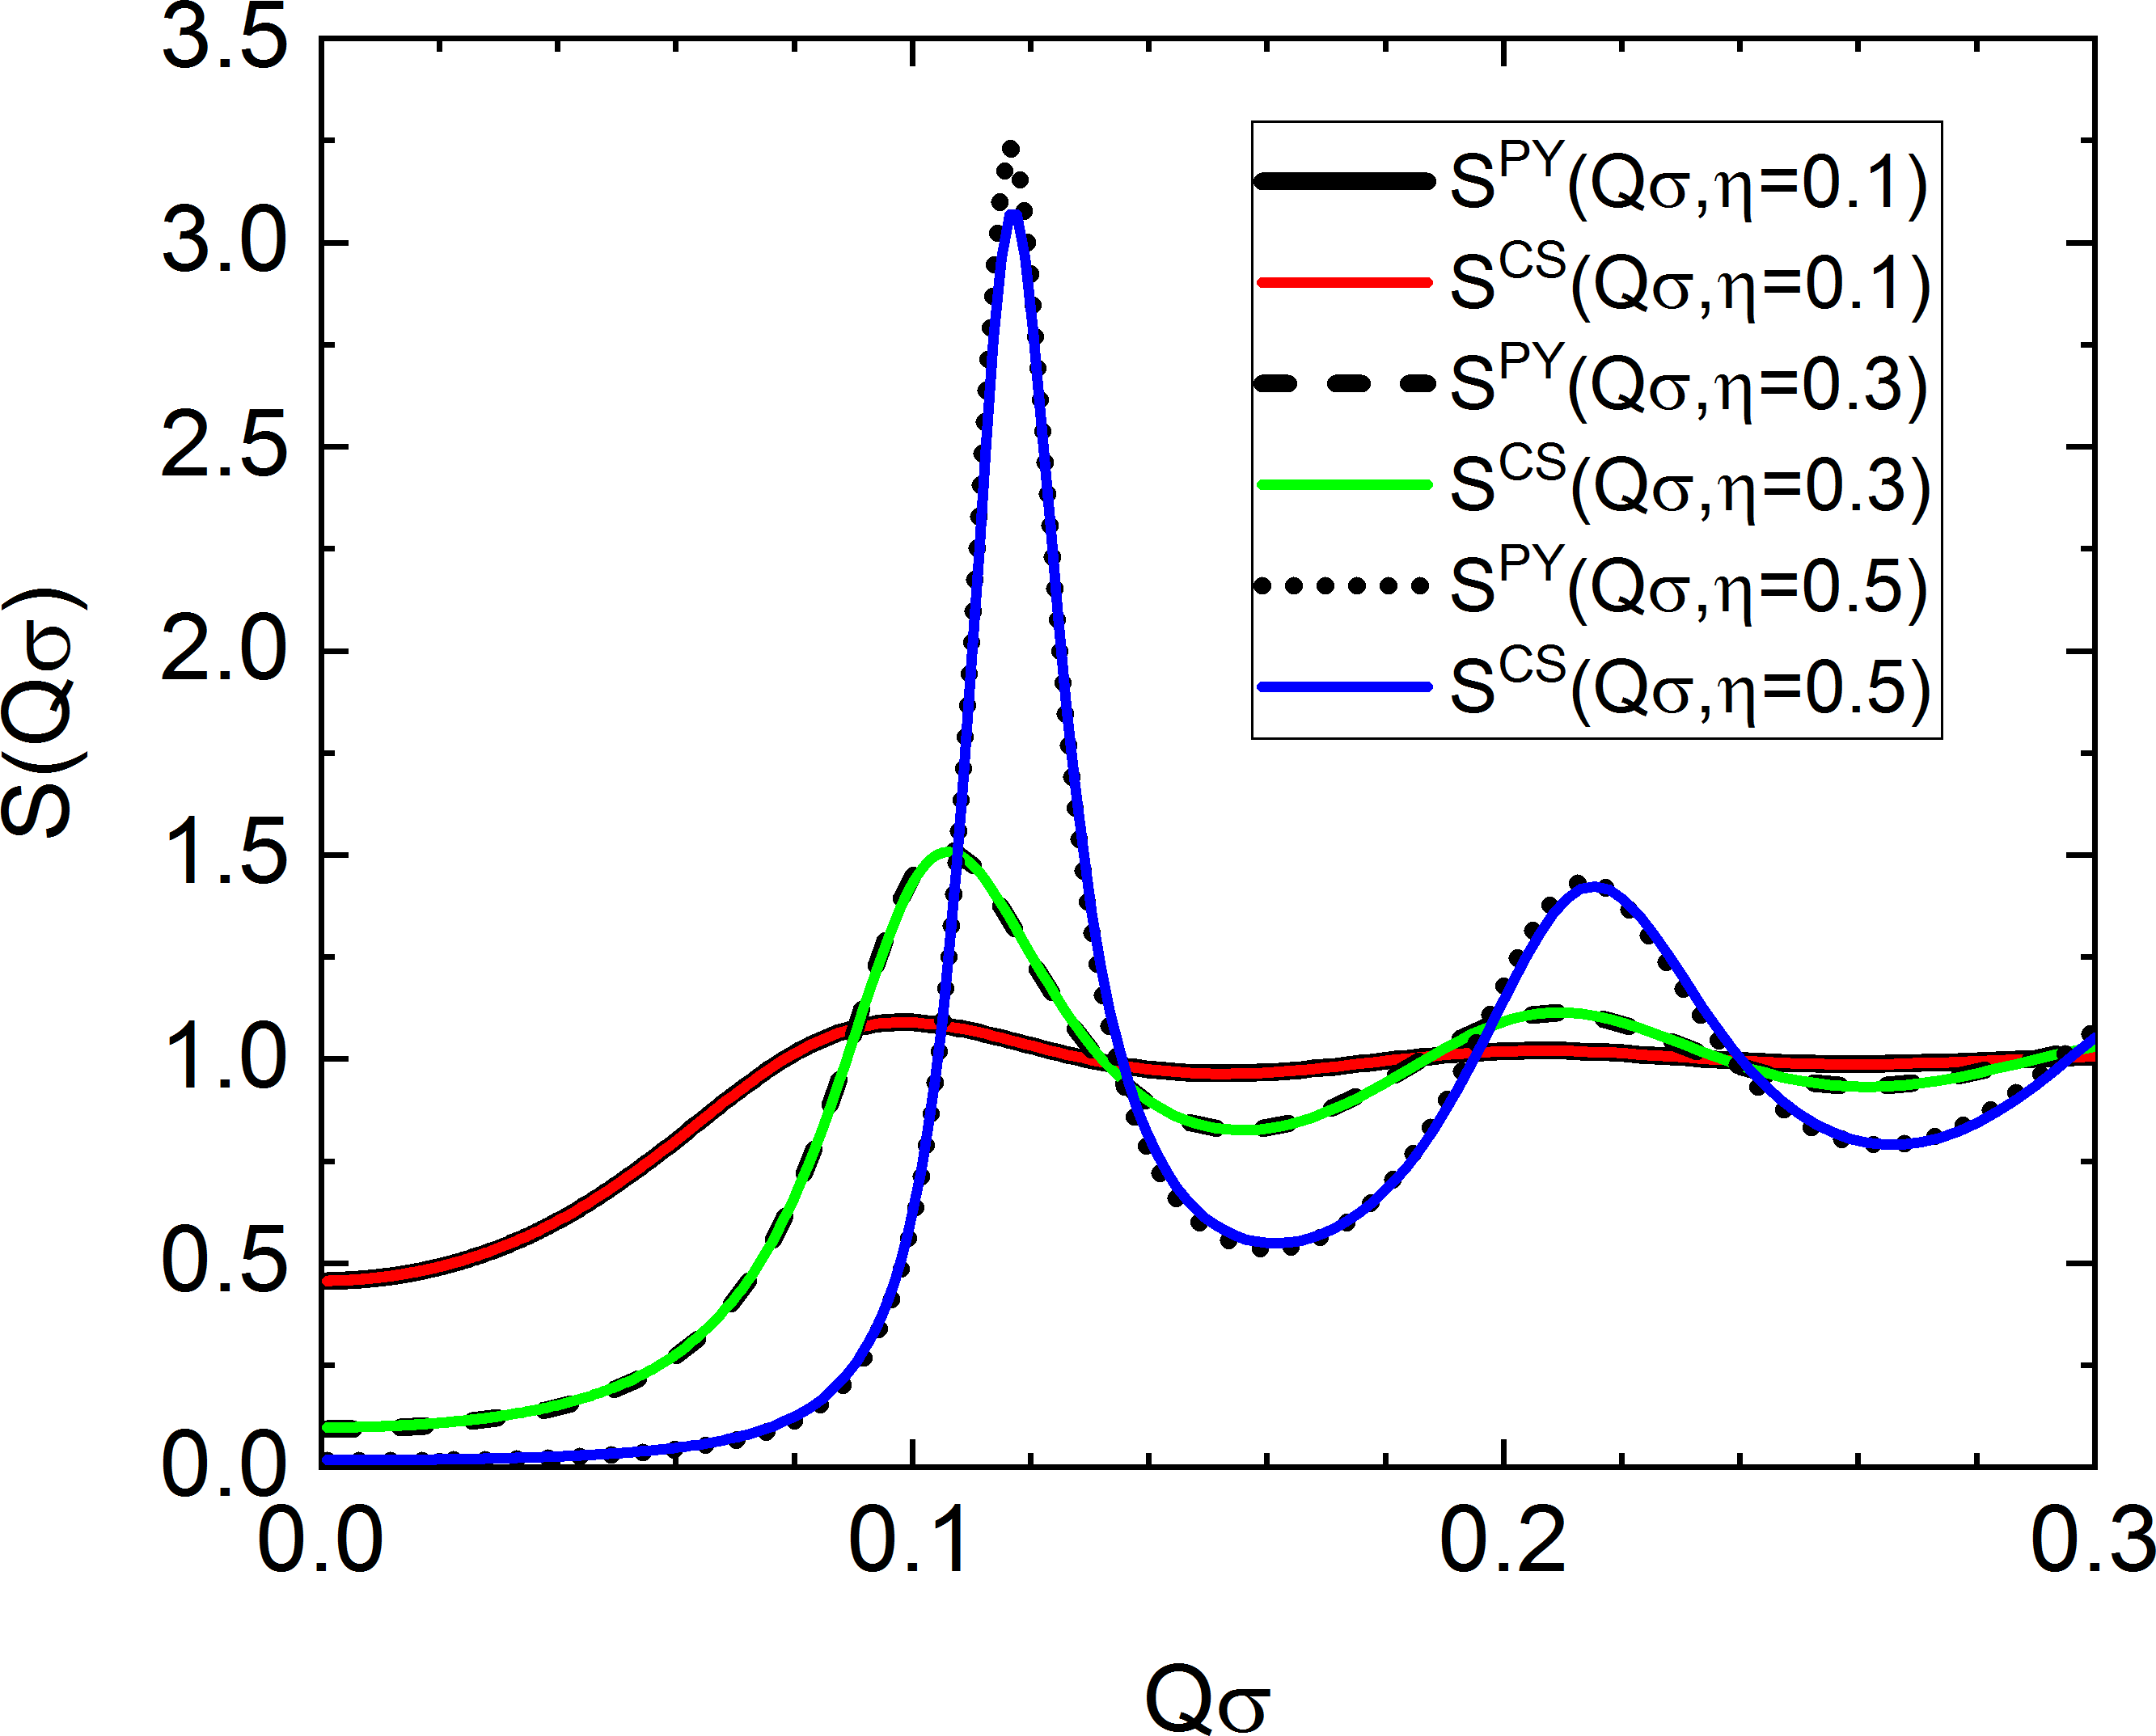
\includegraphics[width=0.46\textwidth]{../images/structure_factor/HardSphere/SQCS.png}}
\hfill
\subfigure[residual between $S^\mathrm{PY}$ and $S^\mathrm{CS}$]{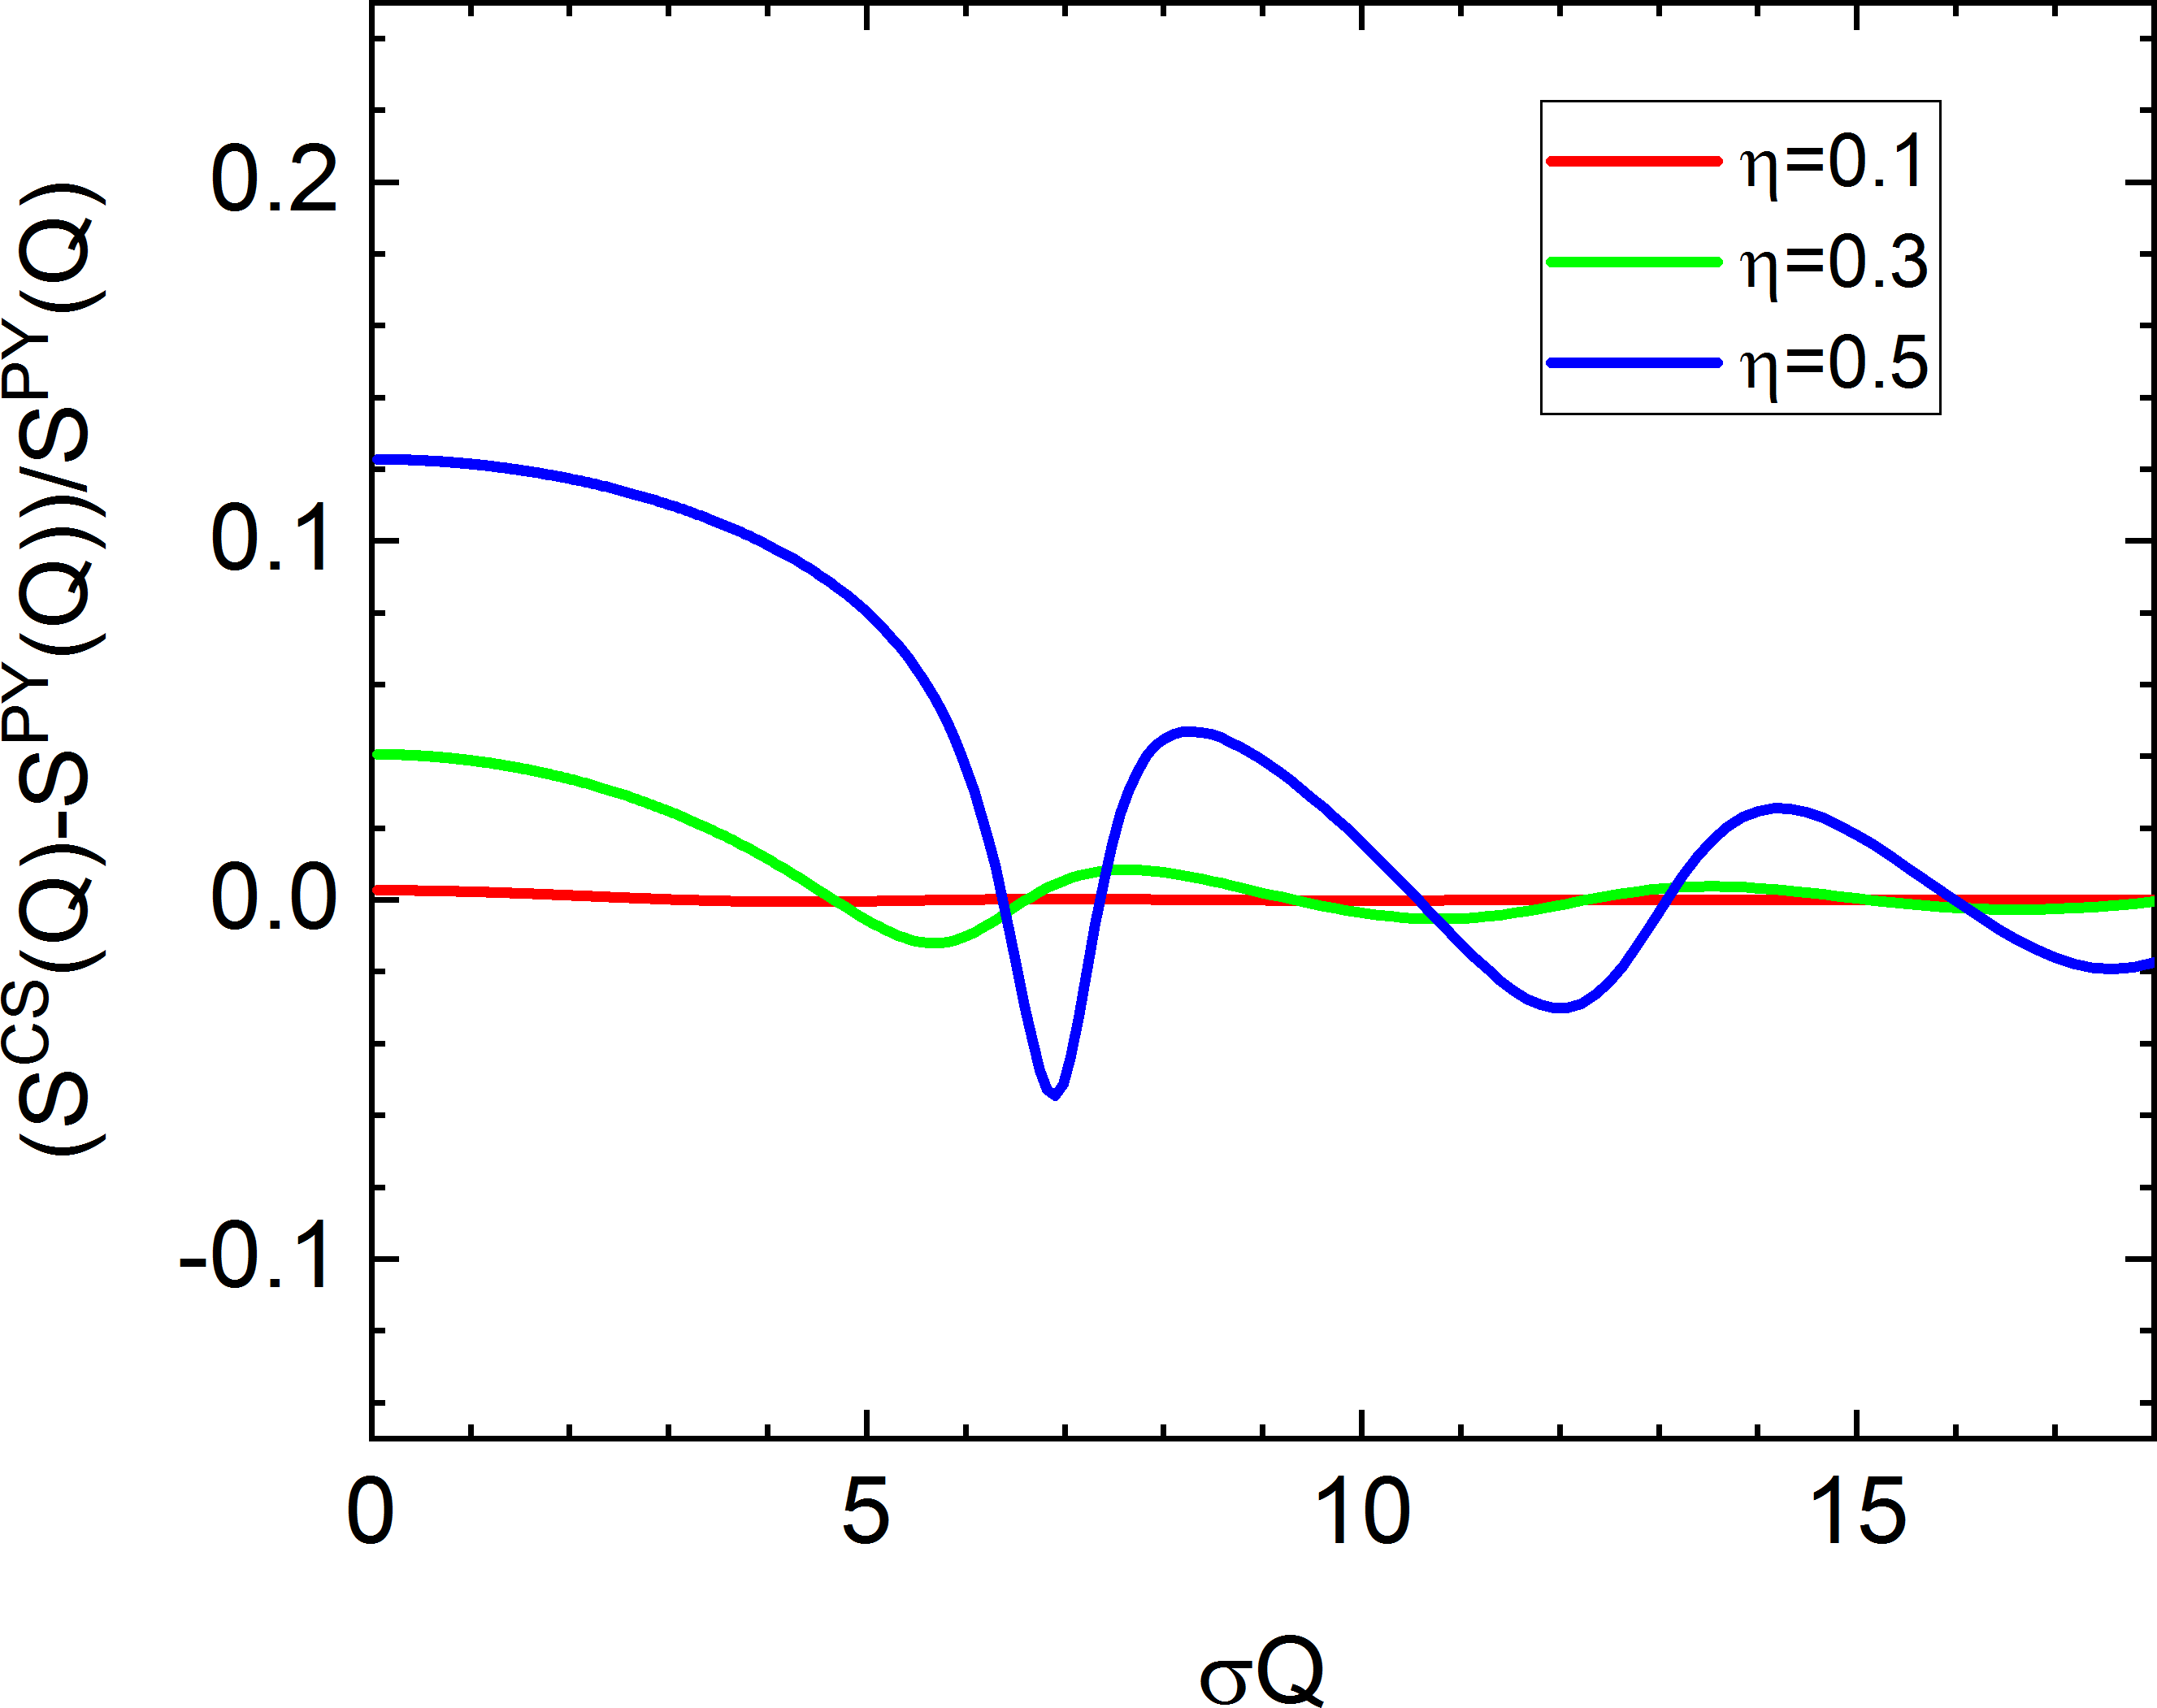
\includegraphics[width=0.48\textwidth]{../images/structure_factor/HardSphere/ResCS.png}} \\
\caption{Comparison between analytical PY solution of hard sphere static structure factor and rational function approximation with a compressibility factor of Carnahan and Starling}
\label{fig:SQ:CS}
\end{figure}

\clearpage
\subsection{Pad\'{e}(4,3) of van Rensburg and S\'{a}nchez} \cite{Rensburg1993,Sanchez1994}

\noindent In this approximation eqs.\ \ref{eq:RFAstart}-\ref{eq:RFAend} are used with $Z=Z^{(4,3)}$, where
\begin{align}
Z^{(4,3)} &= \frac{1+1.024385\eta+1.104537\eta^2-0.4611472\eta^3-0.7430382\eta^4}{1-2.975615\eta+3.007000\eta^2-1.097758\eta^3}
\end{align}

\vspace{5mm}

\hspace{1pt}\\
\underline{Input parameters for \texttt{Hard Sphere (4,3)}:}
\begin{description}
    \item[\texttt{R}]  radius $R$
    \item[\texttt{eta}] volume fraction $\eta$
\end{description}

\noindent
\underline{Note}
\begin{itemize}
\item The structure factor accepts volume fractions between $\eta \in [0,1]$.
\item The threshold packing fraction (packing
fraction at which a glass transition in the hard-sphere fluid takes place) of this model is $\eta^{(4,3)}_0 = 0.5604$  beyond
which no meaningful fluid structure can be derived \cite{Haro2004}.
\end{itemize}

\begin{figure}[htb]
\subfigure[Comparison between $S^\mathrm{PY}$ and $S^{(4,3)}$]{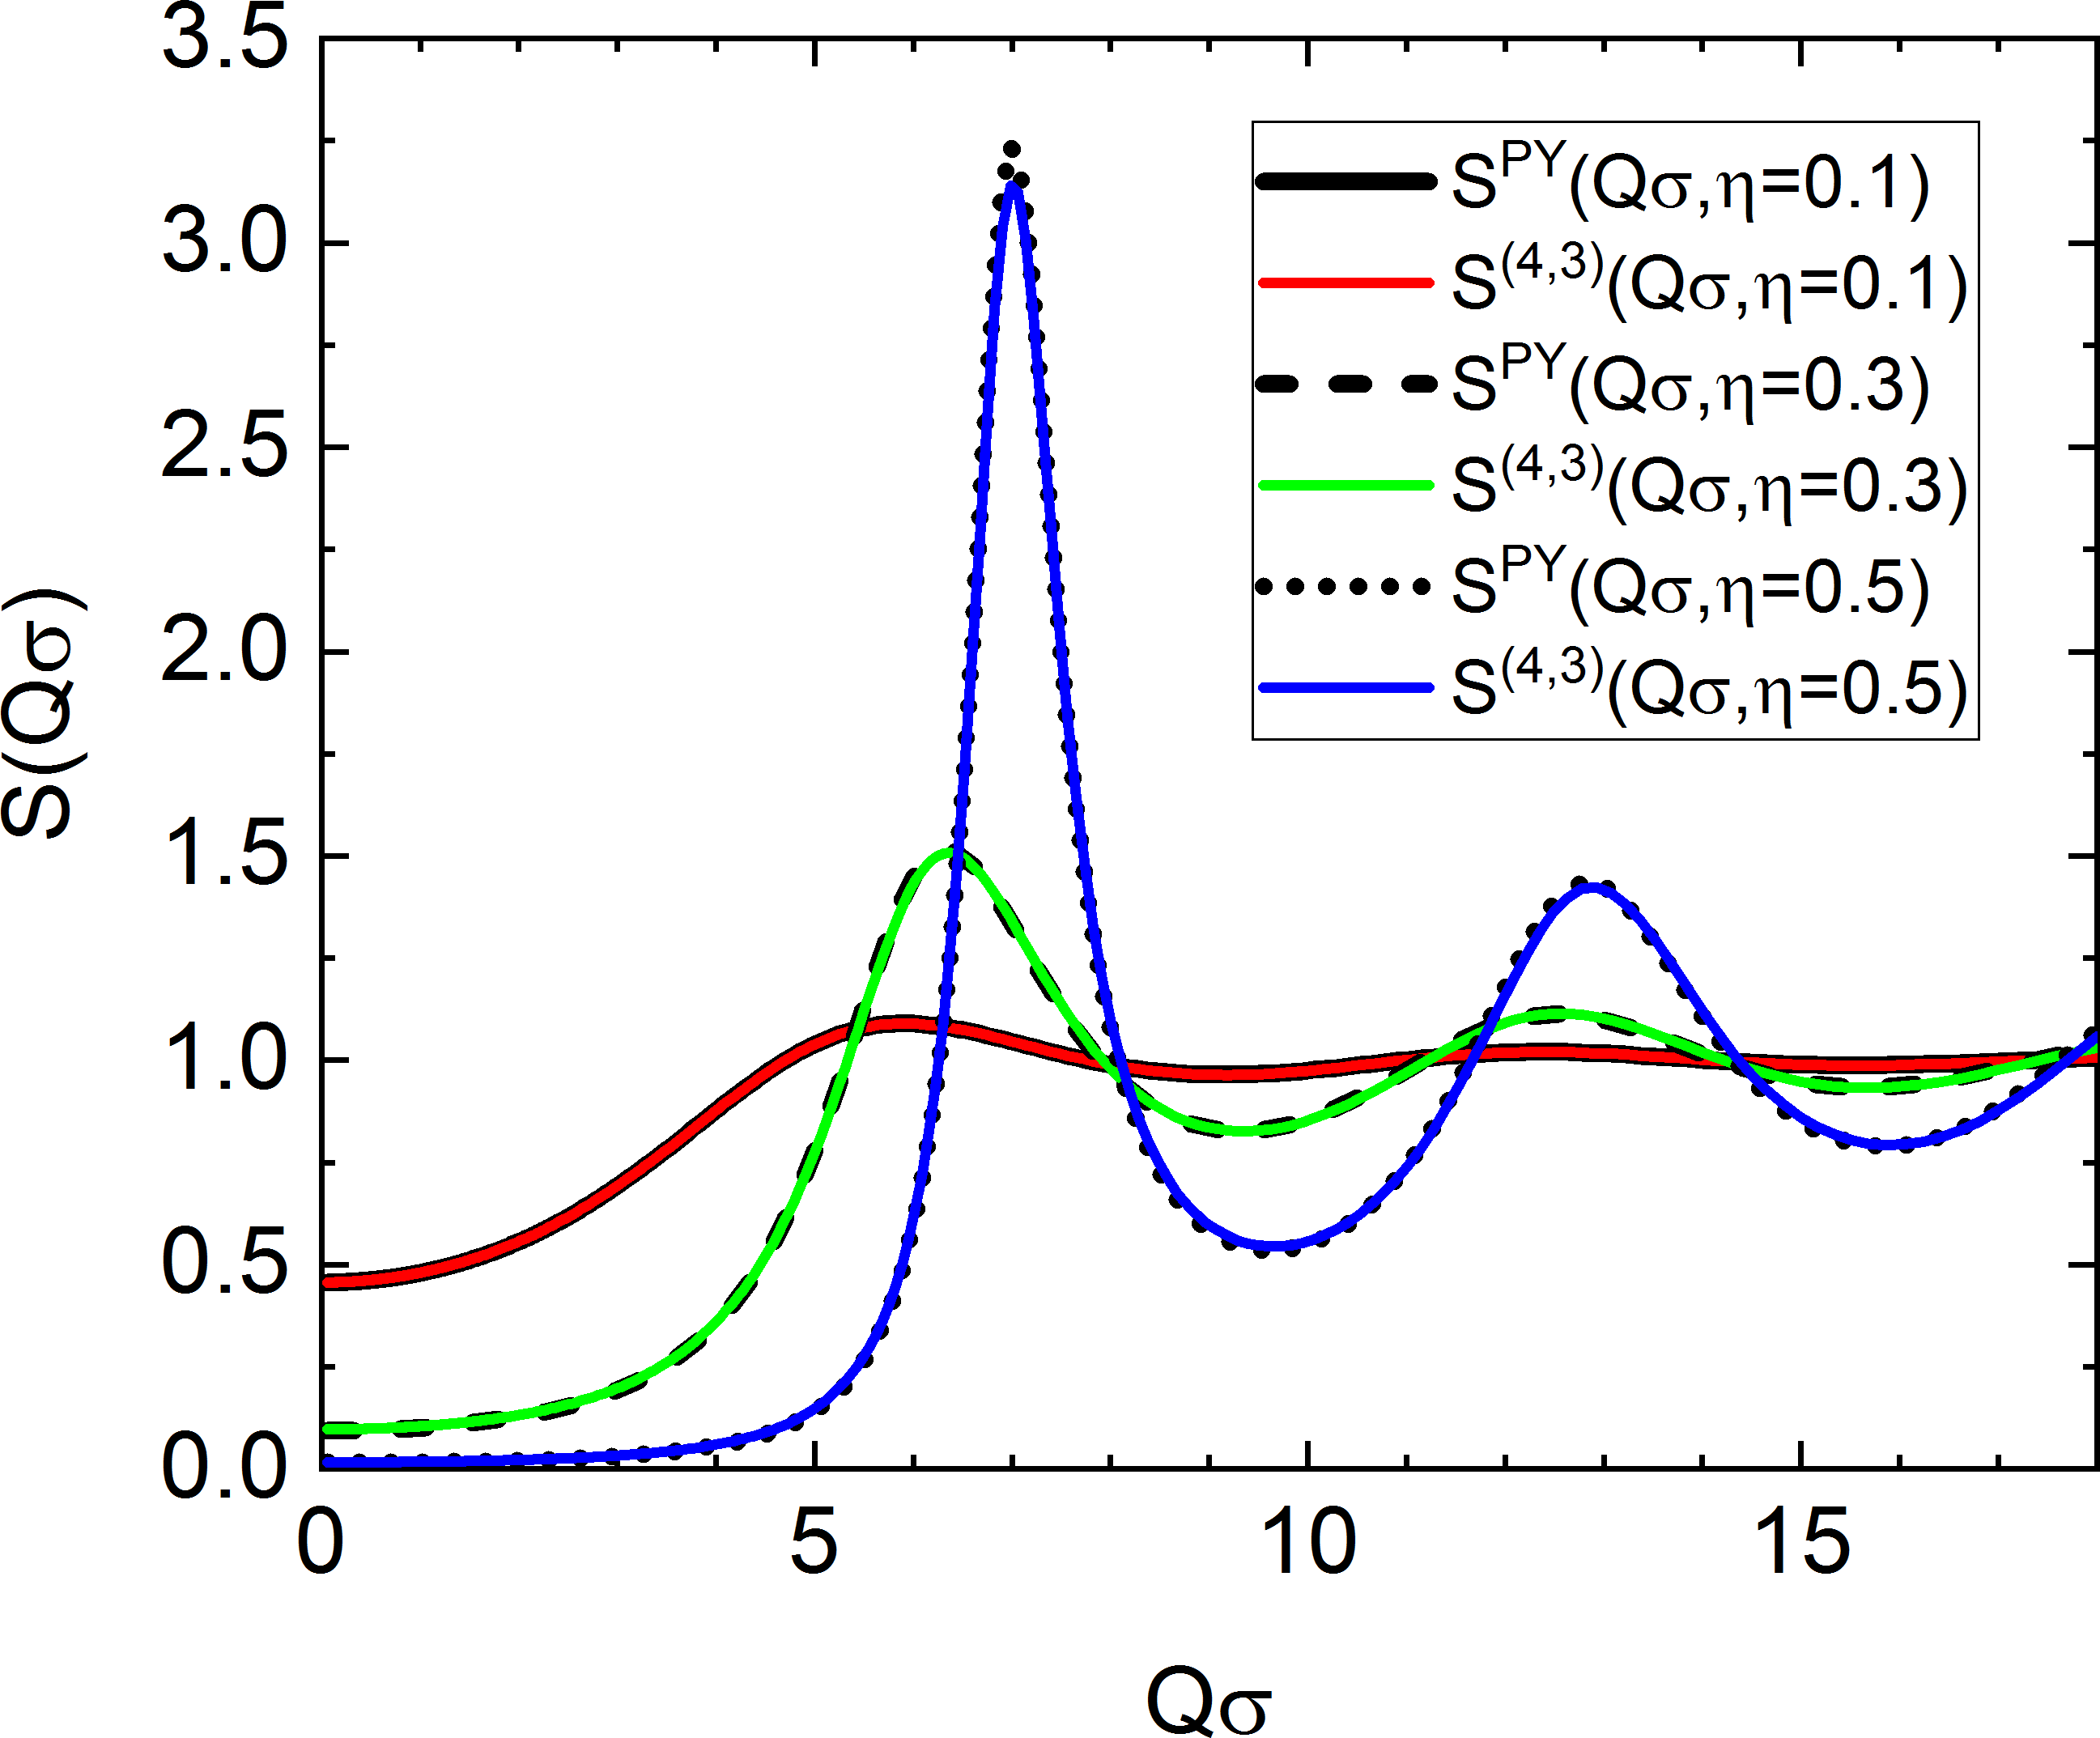
\includegraphics[width=0.46\textwidth]{../images/structure_factor/HardSphere/SQ(4,3).png}}
\hfill
\subfigure[residual between $S^\mathrm{PY}$ and $S^{(4,3)}$]{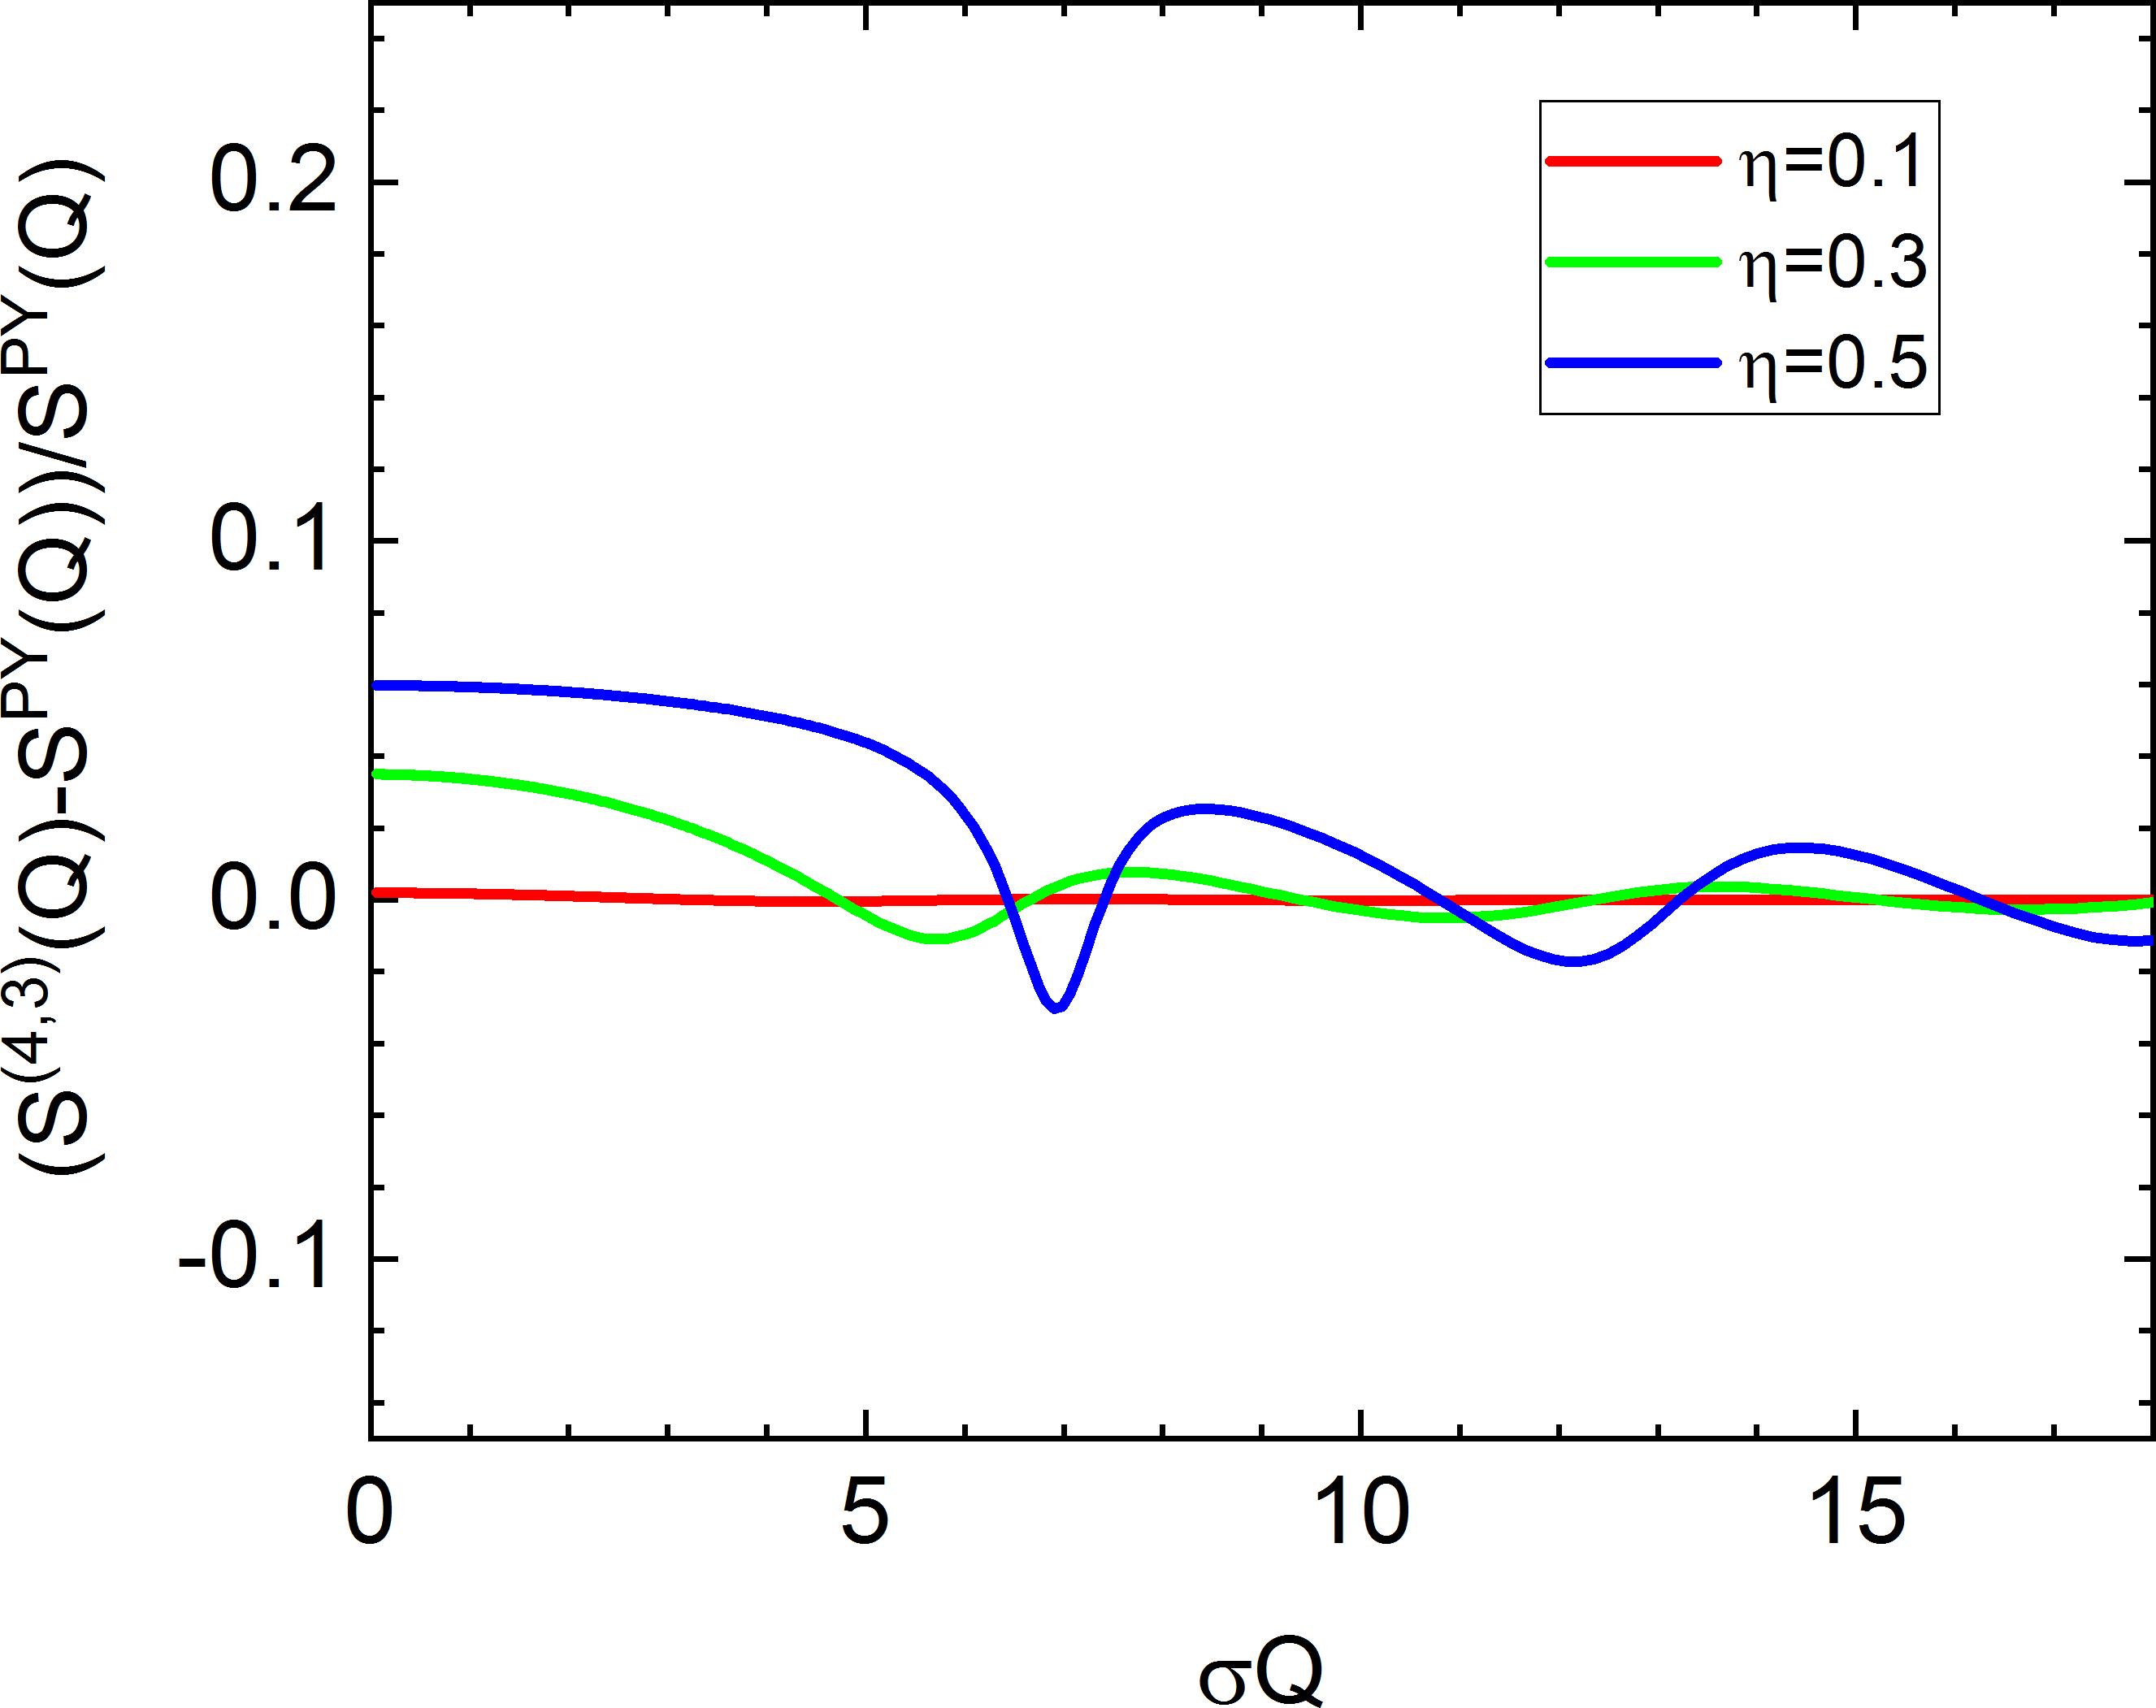
\includegraphics[width=0.48\textwidth]{../images/structure_factor/HardSphere/Res(4,3).png}} \\
\caption{Comparison between analytical PY solution of hard sphere static structure factor and rational function approximation with a compressibility factor of van Rensburg and S\'{a}nchez}
\label{fig:SQ:43}
\end{figure}

\clearpage
\subsection{Malijevsk\'{y} and Veverka} \cite{Malijevsky1999}

\noindent In this approximation eqs.\ \ref{eq:RFAstart}-\ref{eq:RFAend} are used with $Z=Z^\mathrm{MV}$, where
\begin{align}
Z^\mathrm{MV} &= \frac{1 + 1.0560\eta + 1.6539\eta^2 + 0.3262\eta^3}{\left(1- 3.8464\eta + 4.9574\eta^2 -2.1639\eta^3\right)\left(1-\eta\right)^3}
\end{align}

\vspace{5mm}

\hspace{1pt}\\
\underline{Input parameters for \texttt{Hard Sphere (MV)}:}
\begin{description}
    \item[\texttt{R}]  radius $R$
    \item[\texttt{eta}] volume fraction $\eta$
\end{description}

\noindent
\underline{Note}
\begin{itemize}
\item The structure factor accepts volume fractions between $\eta \in [0,1]$.
\item The model lead to physically meaningful structural properties in the whole definition range of volume fractions.
\end{itemize}

\begin{figure}[htb]
\subfigure[Comparison between $S^\mathrm{PY}$ and $S^\mathrm{MV}$]{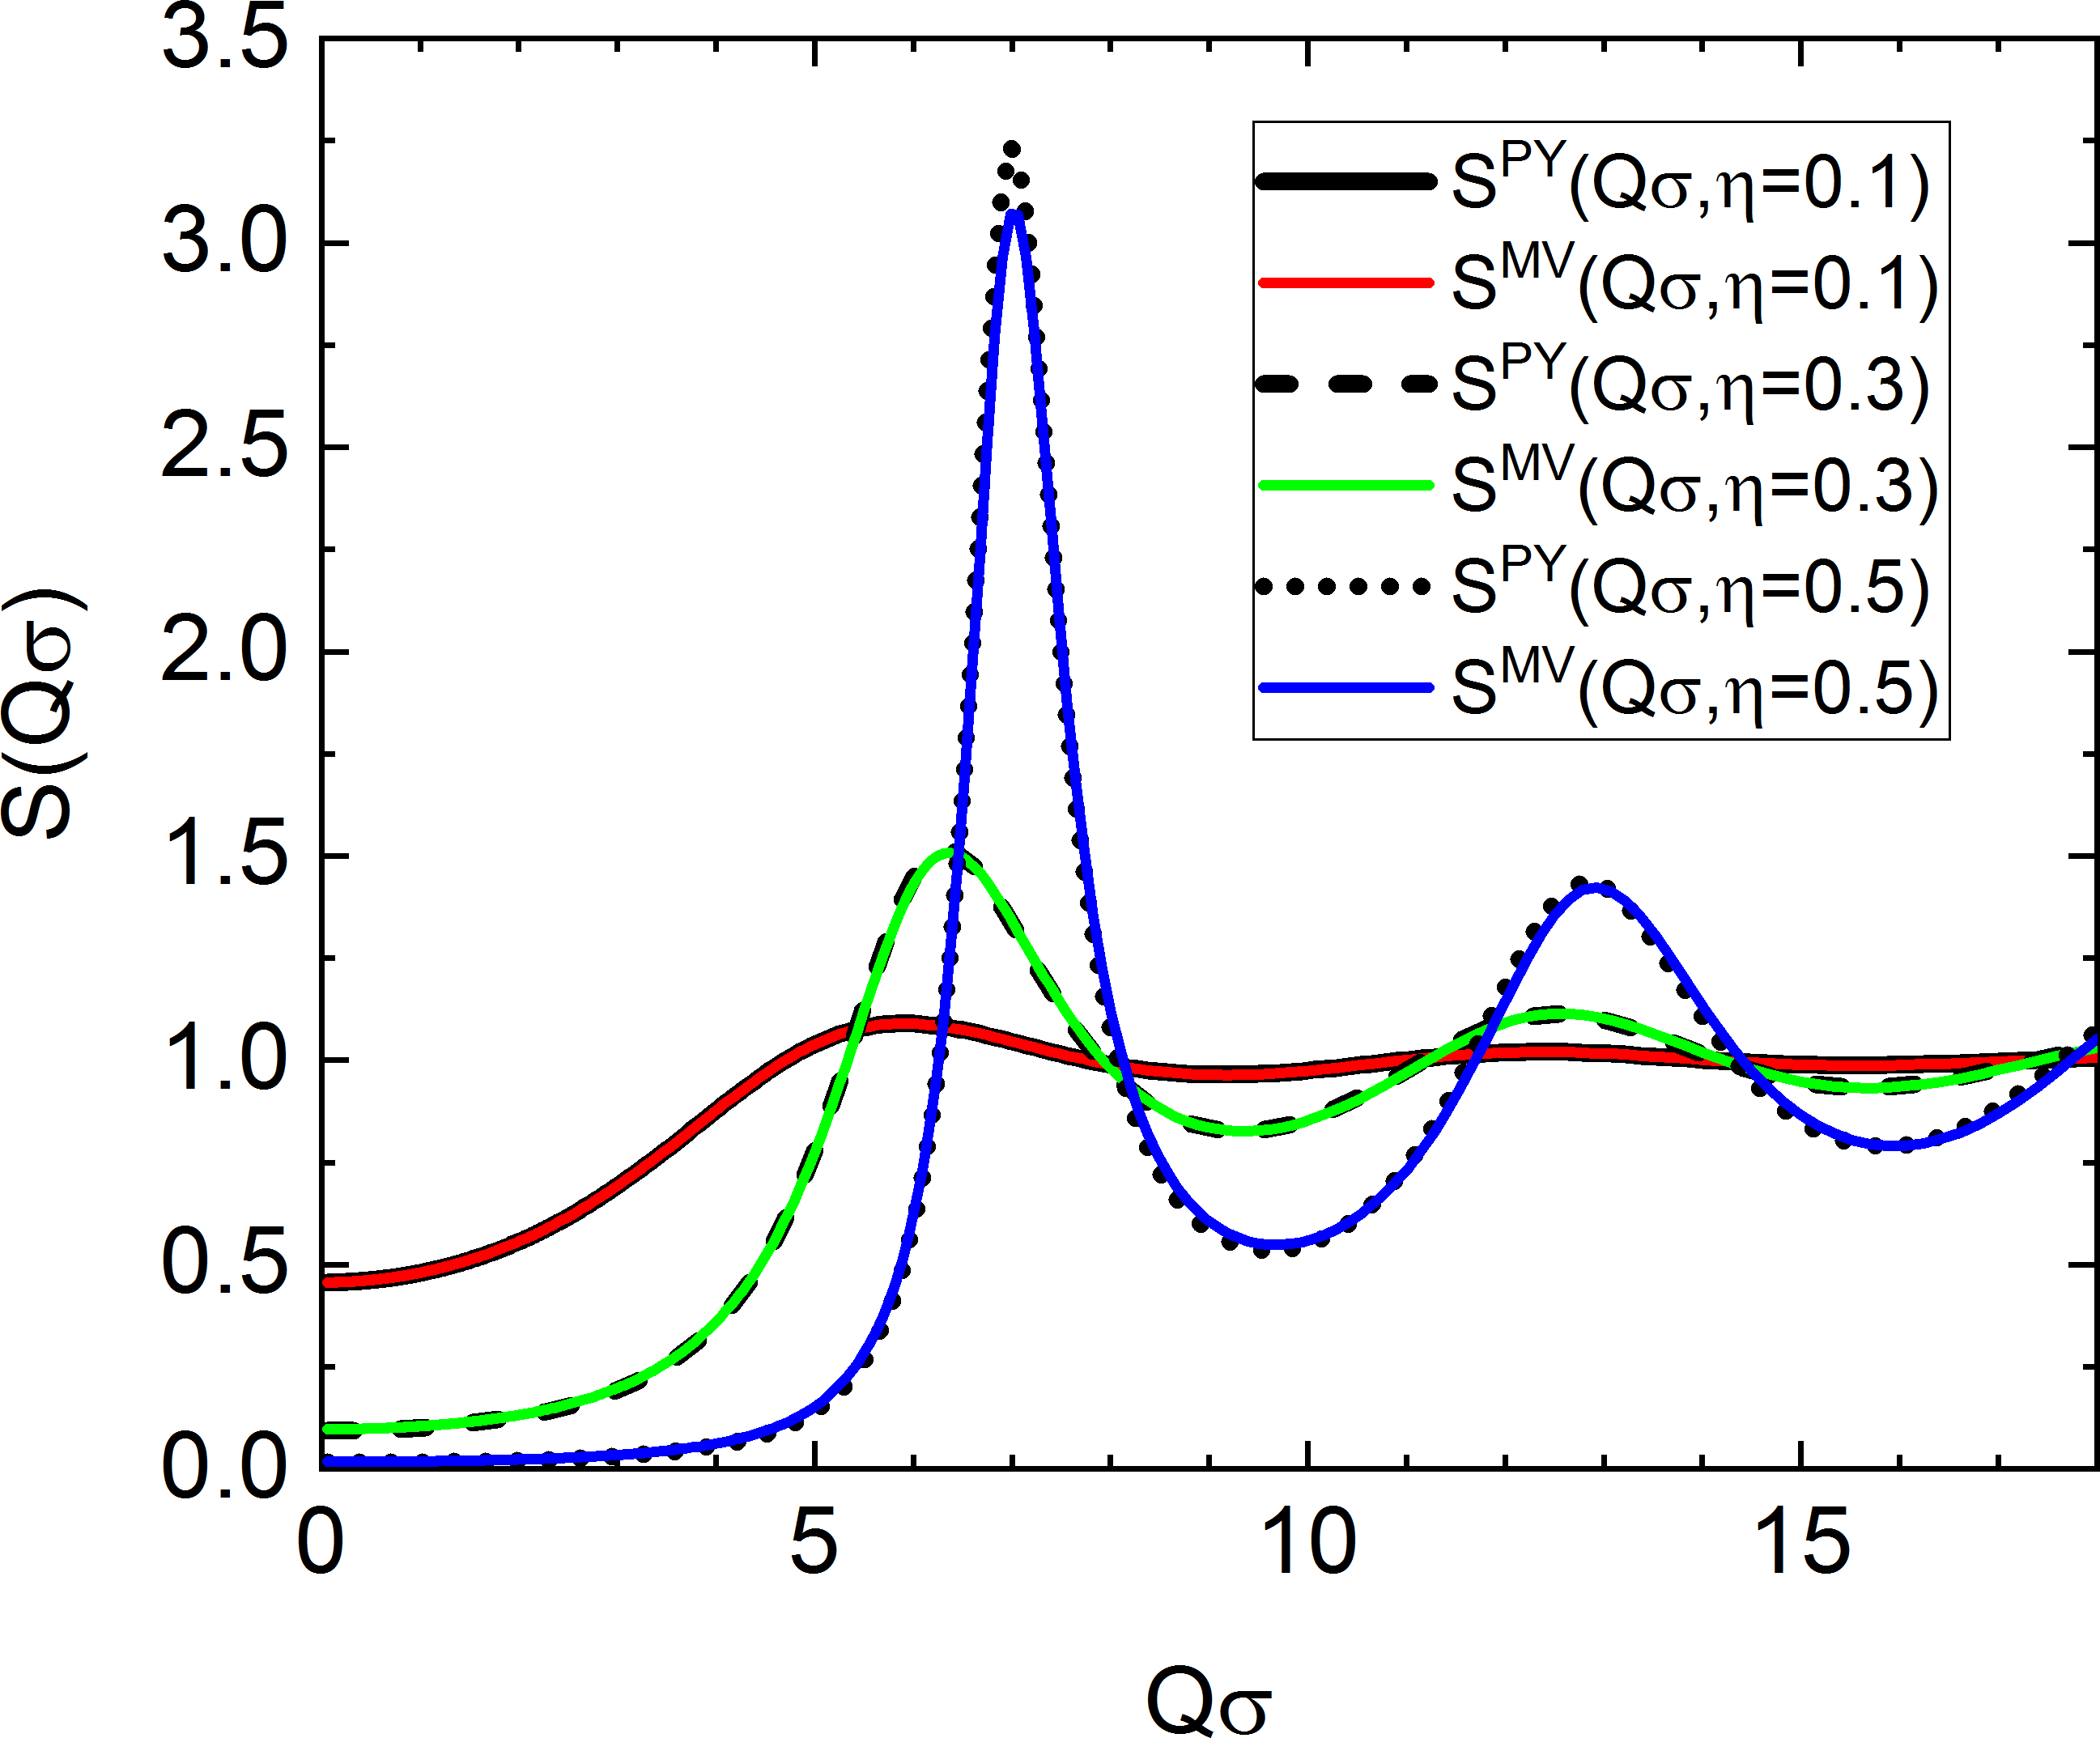
\includegraphics[width=0.46\textwidth]{../images/structure_factor/HardSphere/SQMV.png}}
\hfill
\subfigure[residual between $S^\mathrm{PY}$ and $S^\mathrm{MV}$]{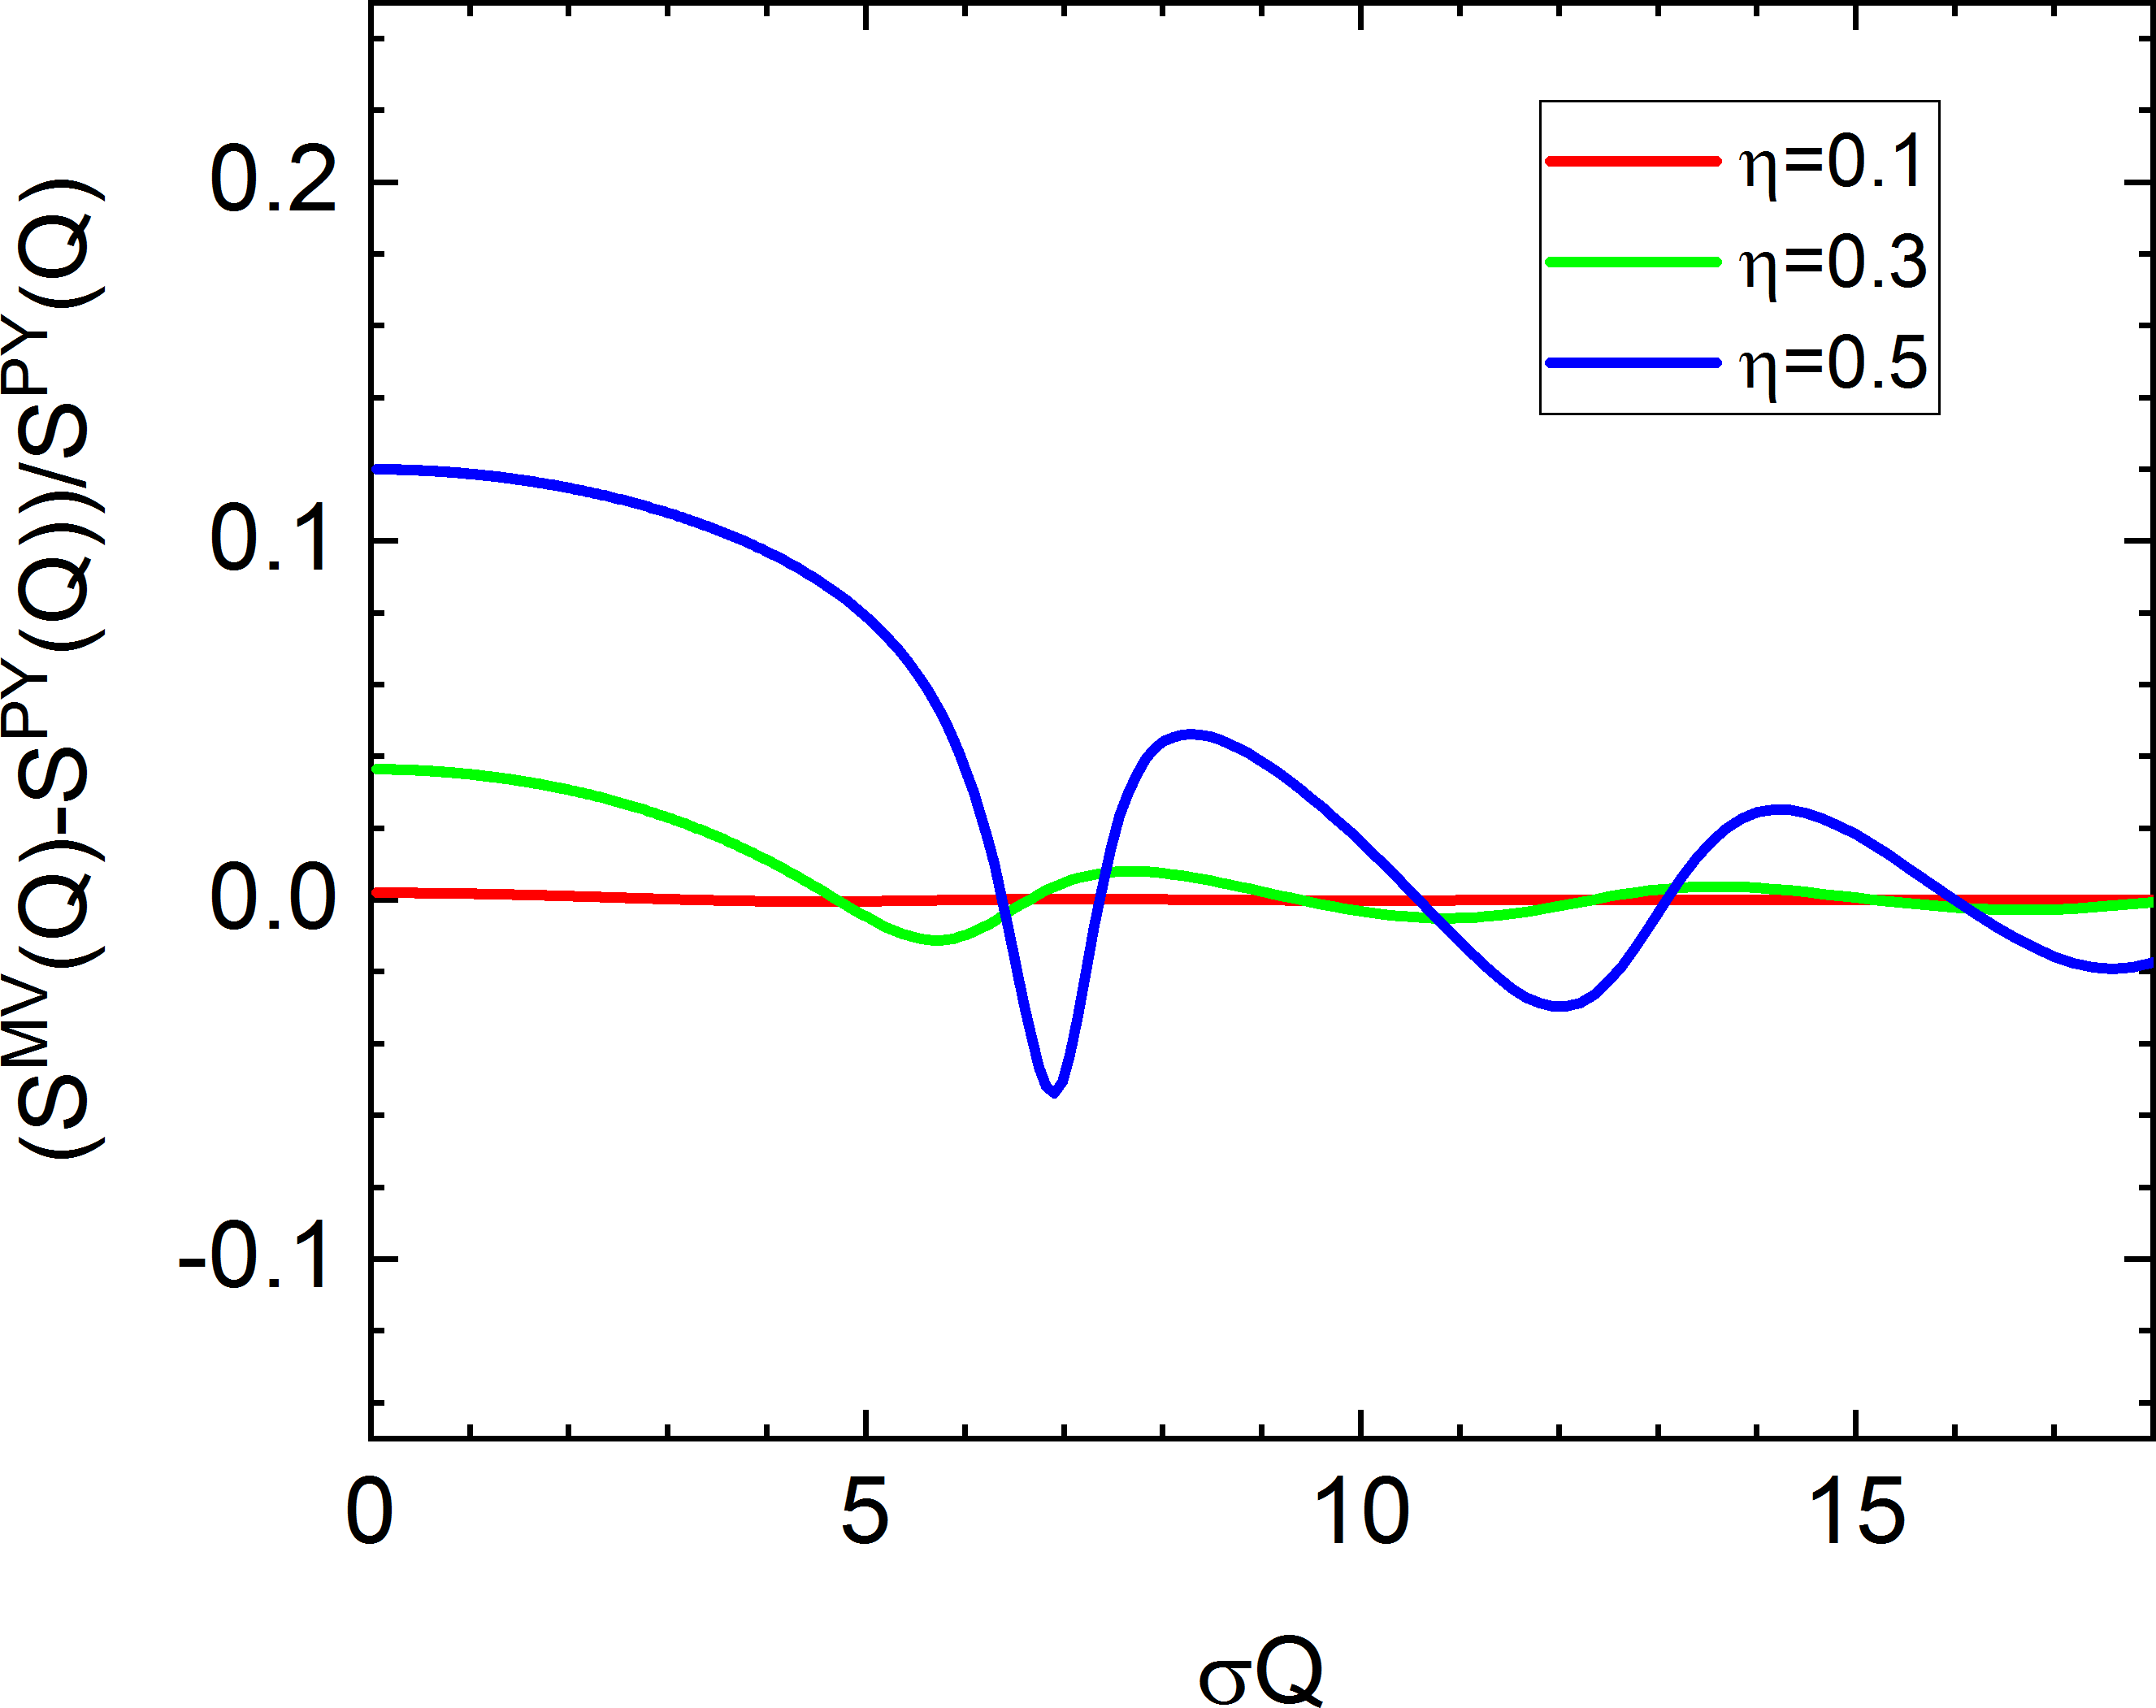
\includegraphics[width=0.48\textwidth]{../images/structure_factor/HardSphere/ResMV.png}} \\
\caption{Comparison between analytical PY solution of hard sphere static structure factor and rational function approximation with a compressibility factor of Malijevsk\'{y} and Veverka}
\label{fig:SQ:MV}
\end{figure}

\clearpage
\subsection{L\'{o}pez de Haro and Robles} \cite{Robles2003}

\noindent In this approximation eqs.\ \ref{eq:RFAstart}-\ref{eq:RFAend} are used with $Z=Z^\mathrm{LHR}$, where
\begin{align}
Z^\mathrm{LHR} &= \frac{1   + 0.153555\eta
                            - 0.428376\eta^2
                            - 2.7987\eta^3
                            - 0.317417\eta^4
                            - 0.105806\eta^5}{1-3.84644\eta + 4.9574\eta^2 - 2.16386\eta^3}
\end{align}

\vspace{5mm}

\hspace{1pt}\\
\underline{Input parameters for \texttt{Hard Sphere (LHR)}:}
\begin{description}
    \item[\texttt{R}]  radius $R$
    \item[\texttt{eta}] volume fraction $\eta$
\end{description}

\noindent
\underline{Note}
\begin{itemize}
\item The structure factor accepts volume fractions between $\eta \in [0,1]$.
\item The threshold packing fraction (packing
fraction at which a glass transition in the hard-sphere fluid takes place) of this model is $\eta^\mathrm{LHR}_0 = 0.5684$  beyond
which no meaningful fluid structure can be derived \cite{Haro2004}.
\end{itemize}

\begin{figure}[htb]
\subfigure[Comparison between $S^\mathrm{PY}$ and $S^\mathrm{LHR}$]{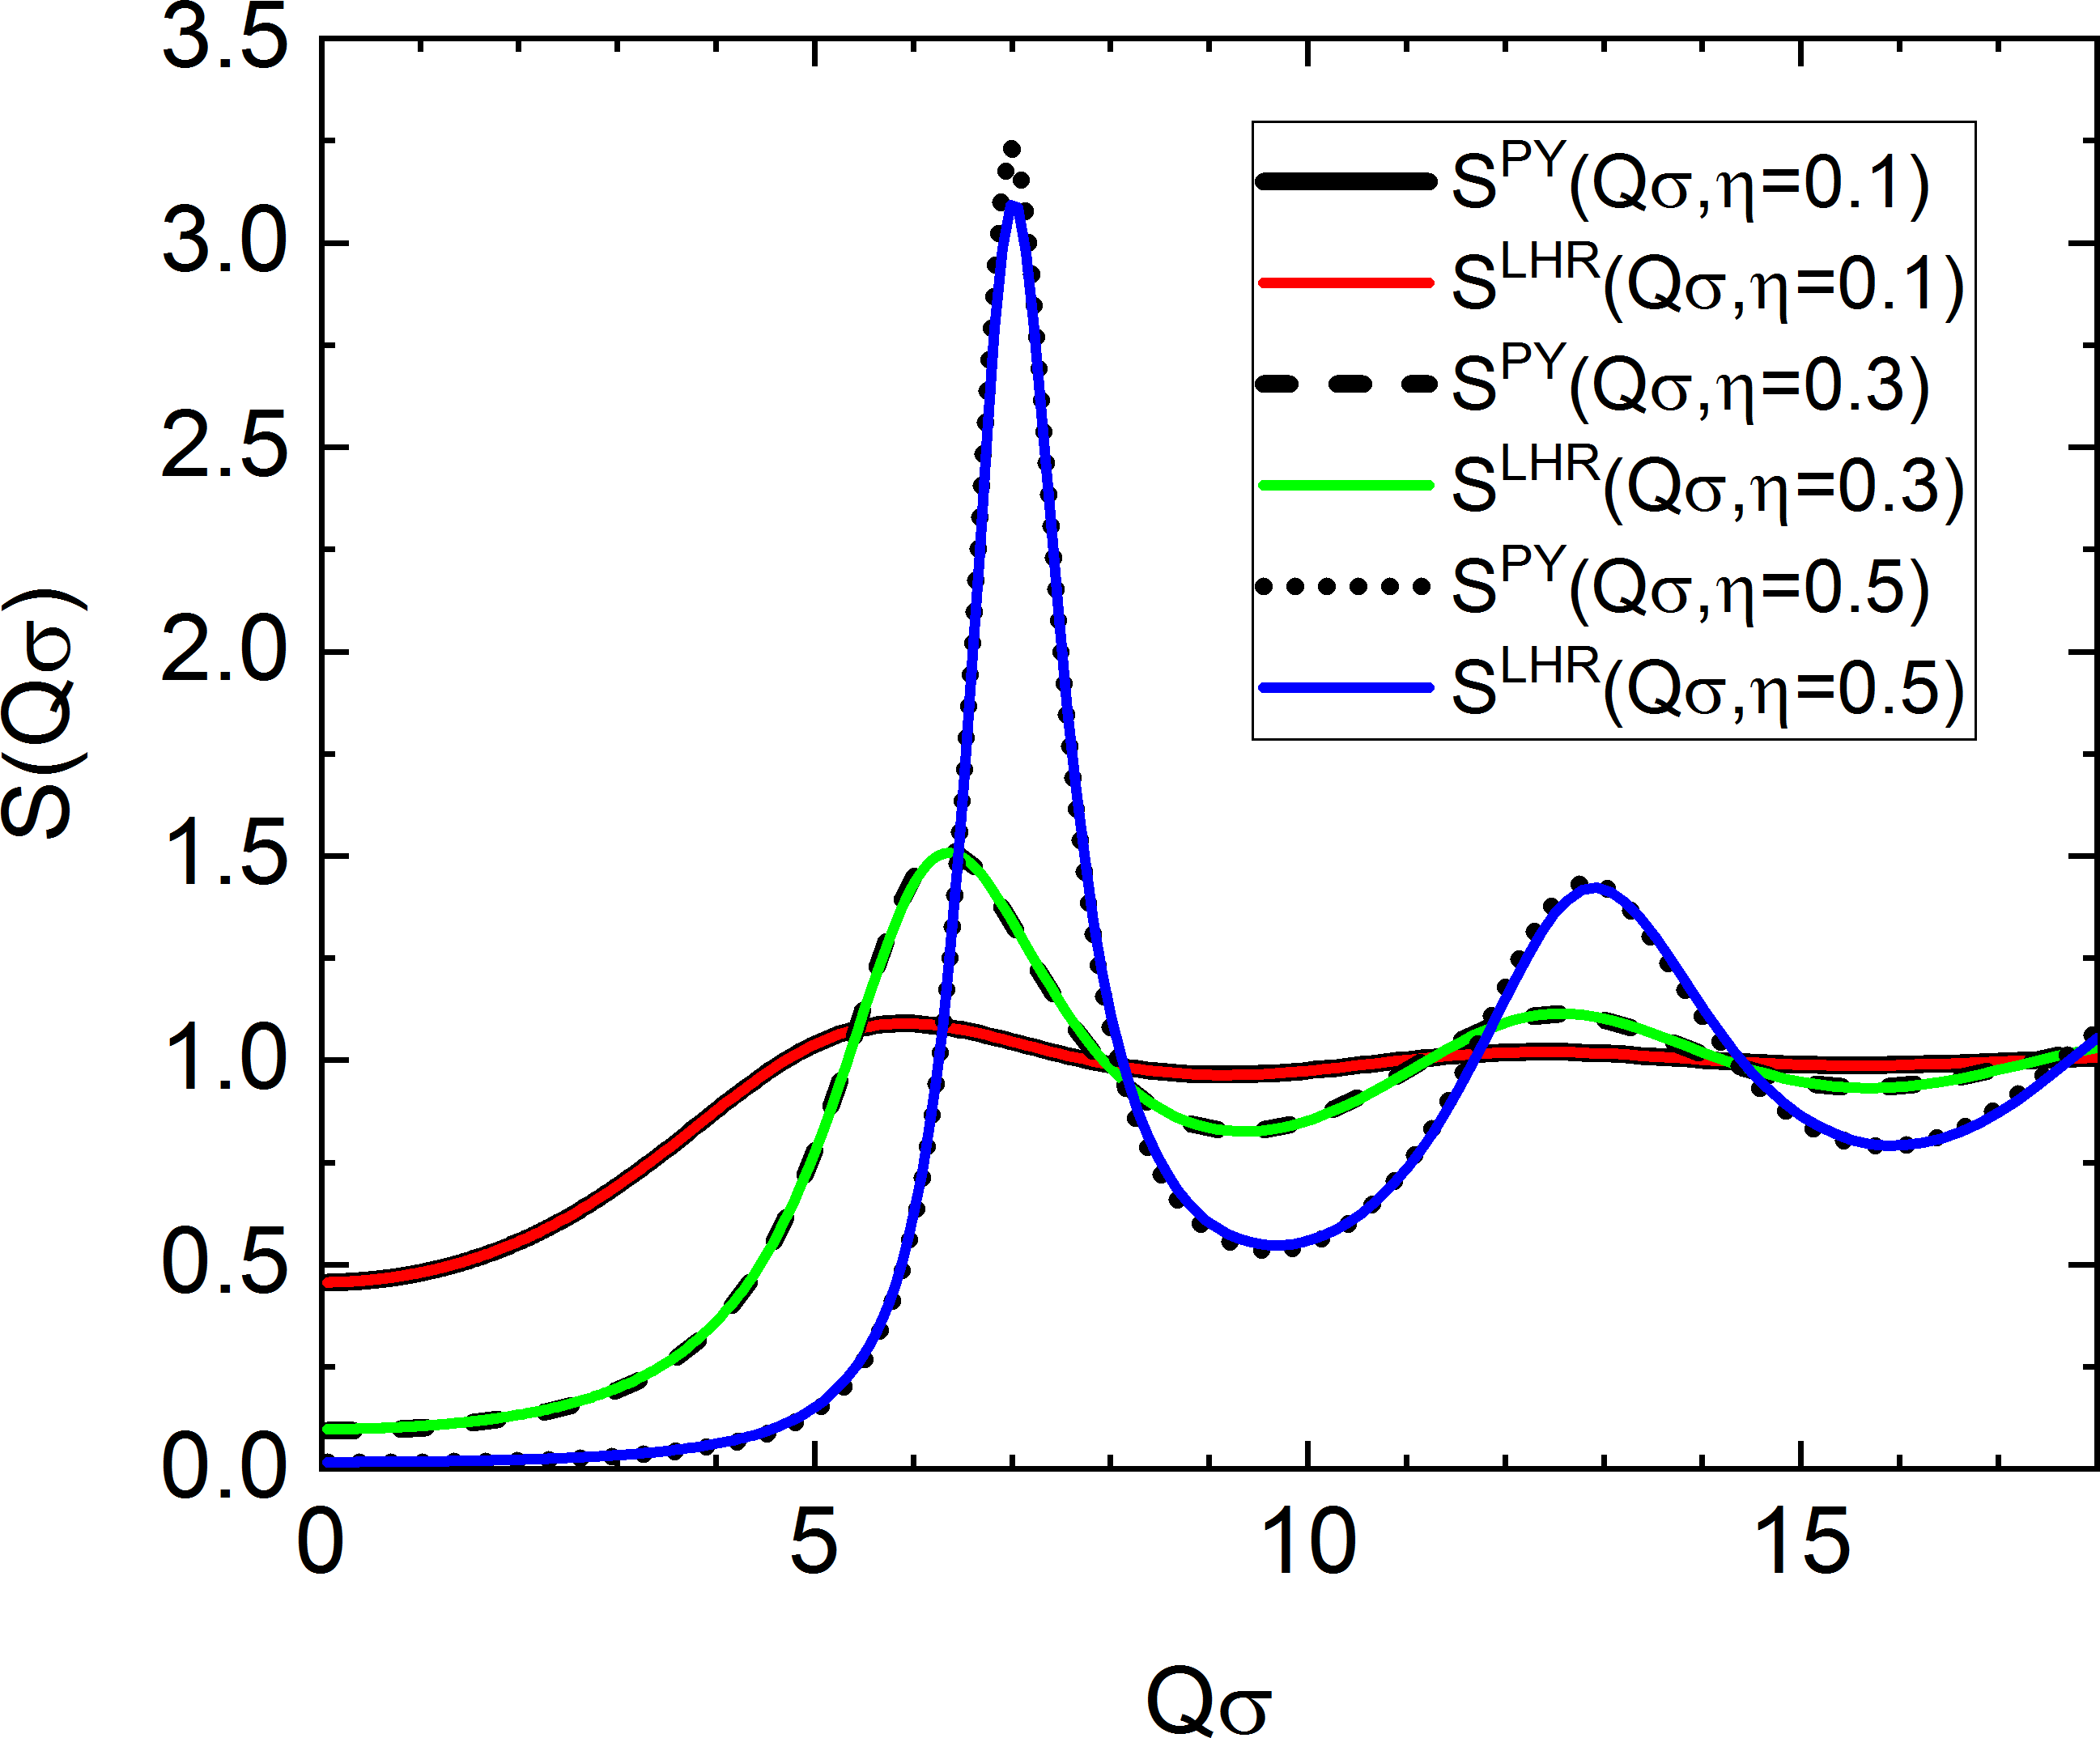
\includegraphics[width=0.46\textwidth]{../images/structure_factor/HardSphere/SQLHR.png}}
\hfill
\subfigure[residual between $S^\mathrm{PY}$ and $S^\mathrm{LHR}$]{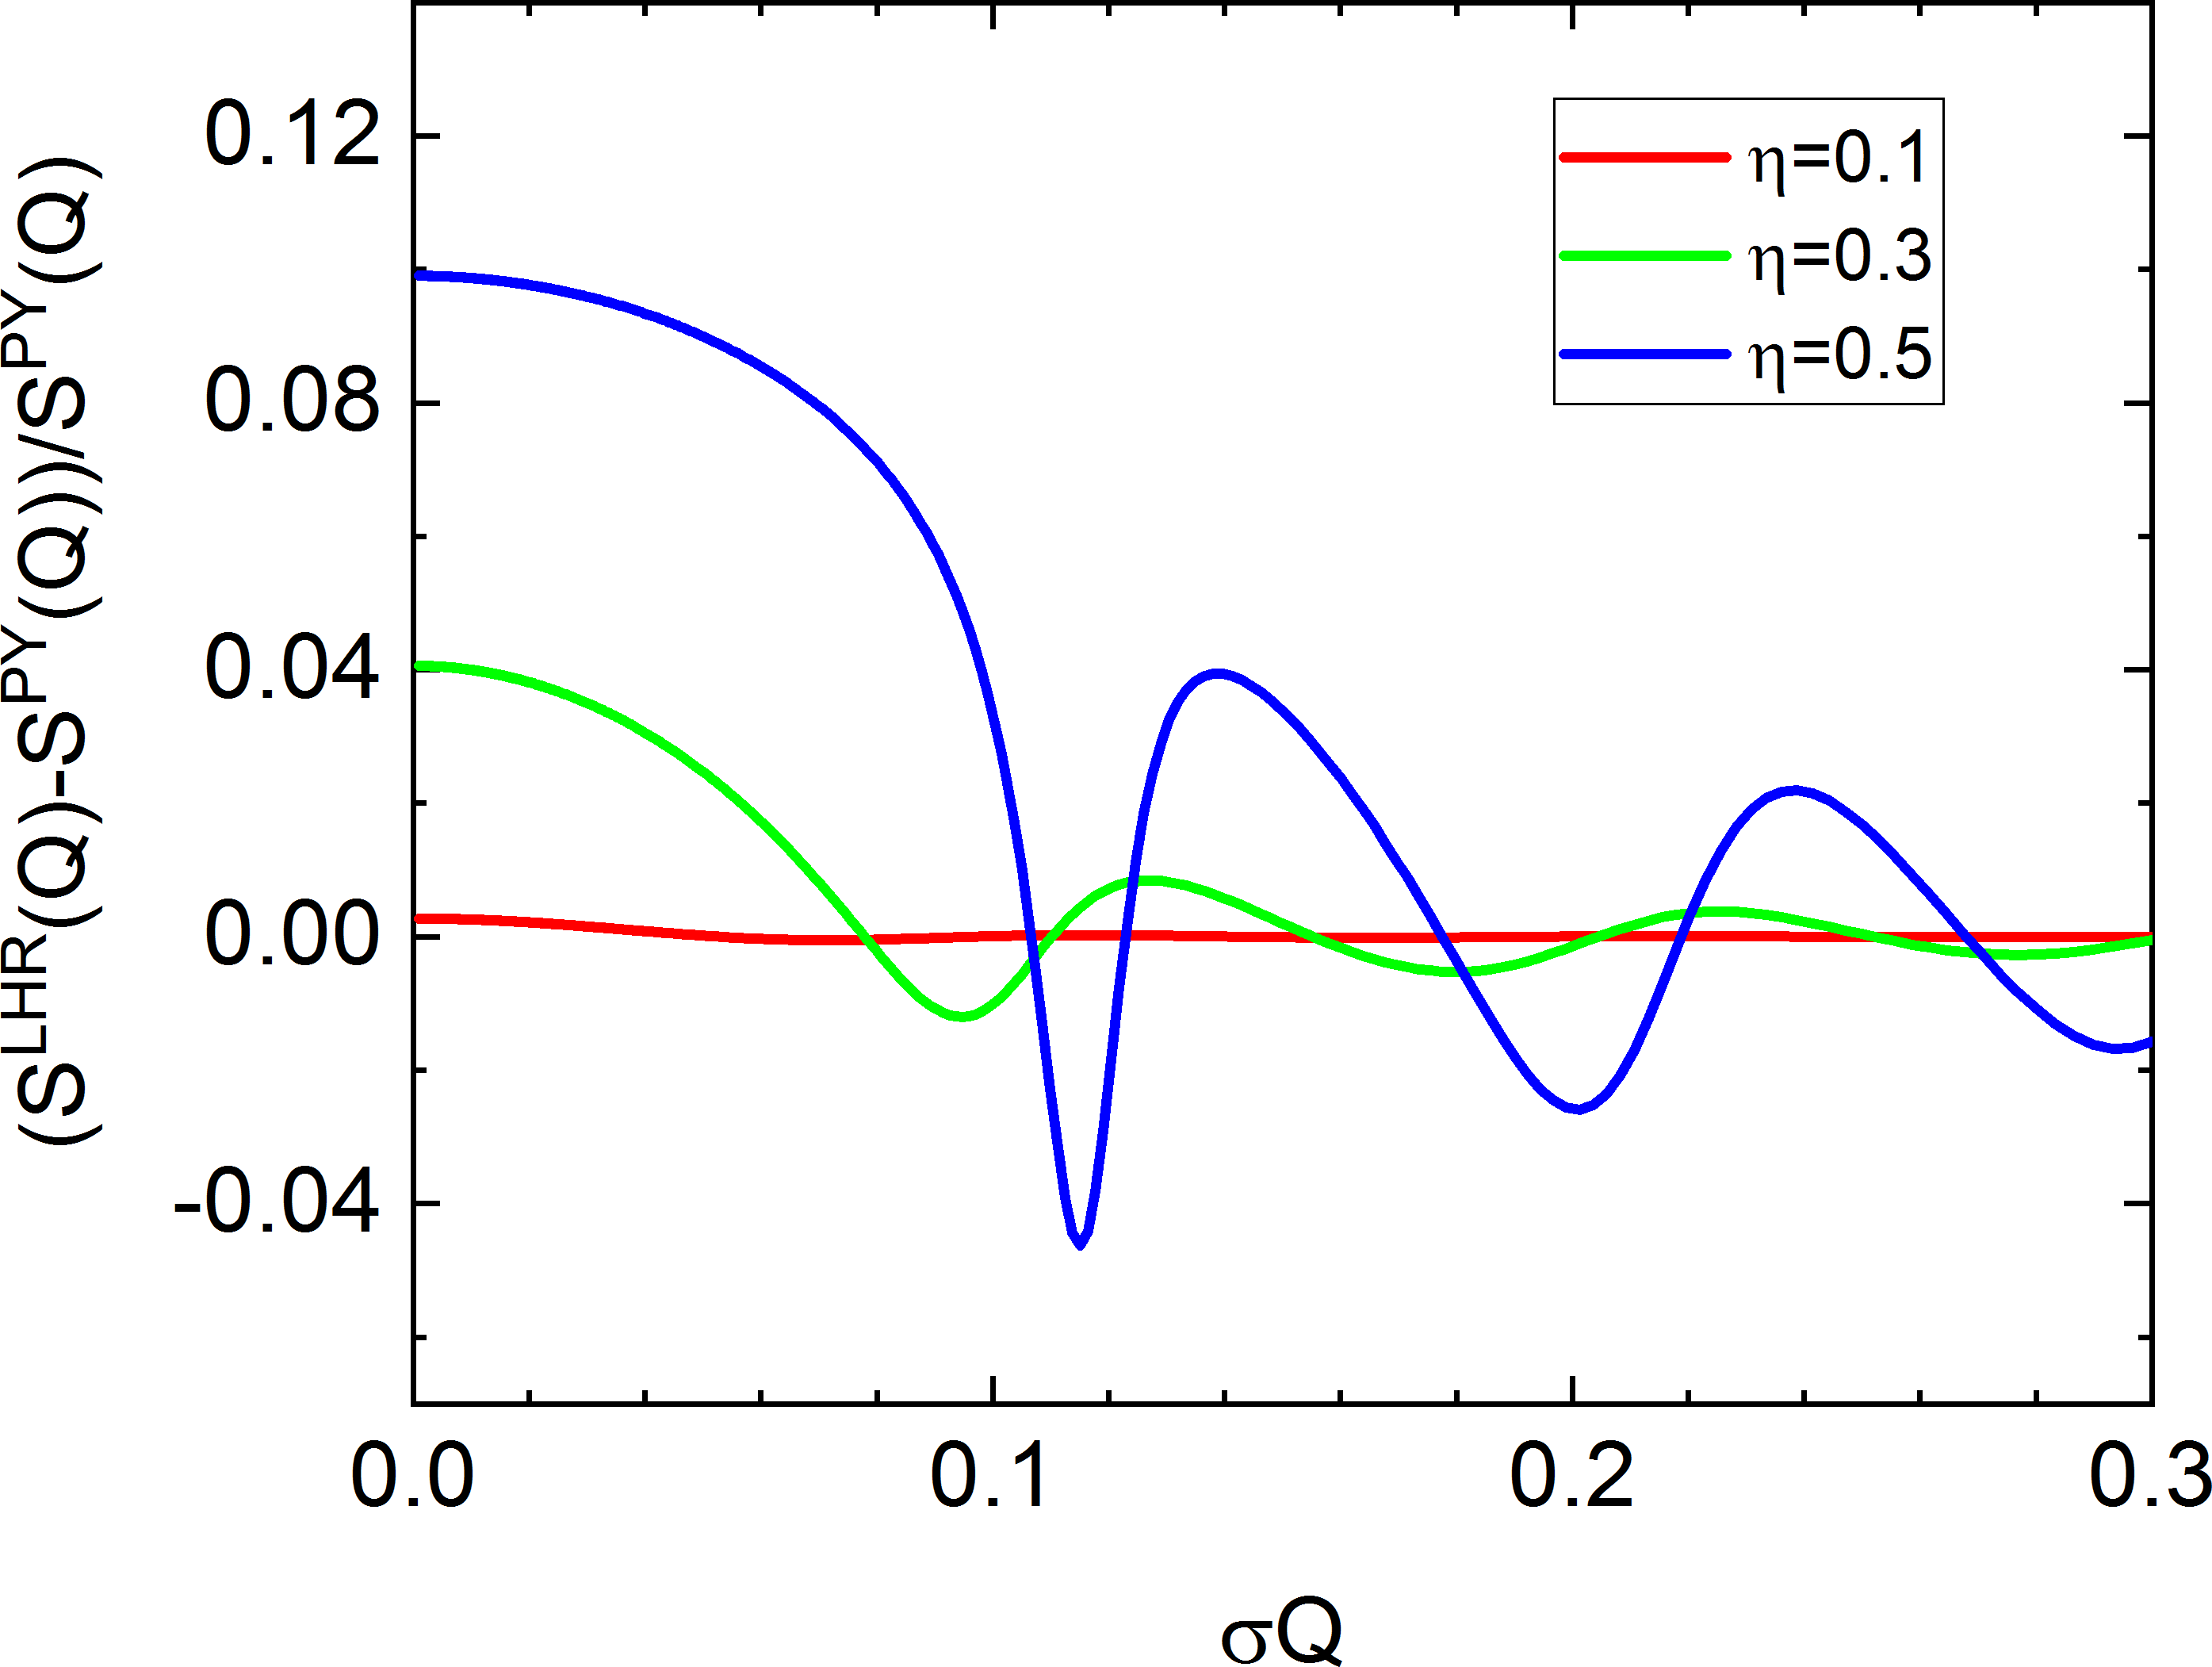
\includegraphics[width=0.48\textwidth]{../images/structure_factor/HardSphere/ResLHR.png}} \\
\caption{Comparison between analytical PY solution of hard sphere static structure factor and rational function approximation with a compressibility factor of L\'{o}pez de Haro and Robles}
\label{fig:SQ:LHR}
\end{figure}

\clearpage
\subsection{Grundke and Henderson} ~\\

\noindent In this approximation the structure factor in the Percus Yevick approximation is corrected to have thermodynamic consistency \cite{Henderson1975} so that both routes leads to the expression of Carnahan and Starling 
$pV/Nk_BT=\frac{1+\eta+\eta^2-\eta^3}{\left(1-\eta\right)^3}$
\begin{align}
\sigma &= 2R\\
\left(\sigma_0/\sigma\right)^3 &= 1-\eta/16\\
\eta_0 &= \eta (1-\eta/16) \\
g_0(s,\eta_0) &\simeq \frac{1+\eta_0/2}{\left(1-\eta_0\right)^2} - \frac{9}{2}\eta_0\frac{1+\eta_0}{\left(1-\eta_0\right)^3}(s-1) \\
\frac{C}{\sigma} &= \frac{2-\eta}{2(1-\eta)^3} - g_0(\sigma/\sigma_0,\eta_0) \\
\frac{12\eta C}{m\sigma_0^2} &= \frac{(1-\eta)^4}{1+4\eta+4\eta^2-4\eta^3+\eta^4} - \frac{(1-\eta_0)^4}{(1+2\eta_0)^2} \nonumber \\
&= 24\eta_0\int_0^{\sigma/\sigma_0} g_0(s,\eta_0)s^2 \mathrm{d}s \\
S^\mathrm{GH}(Q,\sigma,\eta) &= S^\mathrm{PY}(Q,\sigma_0,\eta_0) + \frac{6\eta}{\pi\sigma^3}\tilde{h}_\mathrm{GH}(Q) \\
\tilde{h}_\mathrm{GH}(Q)  &= -\frac{4\pi\sigma_0}{Q\sigma_0} \int_1^{\sigma/\sigma_0} sg_0(s,\eta_0)\sin(Q\sigma_0 s)\mathrm{d}s\\
&+ \frac{2\pi\sigma^3}{Q\sigma}\frac{C}{\sigma} \left\{ \frac{\cos (Q\sigma)}{\sigma}\left[\frac{k+m}{m^2+(Q+m)^2}+\frac{Q-m}{m^2+(Q-m)^2}\right]\right.\nonumber \\
& + \left. \frac{\sin (Q\sigma)}{\sigma}\left[\frac{m}{m^2+(Q+m)^2}+\frac{m}{m^2+(Q-m)^2}\right]\right\}\nonumber 
\end{align}

\vspace{5mm}

\hspace{1pt}\\
\underline{Input parameters for \texttt{Hard Sphere (GH)}:}
\begin{description}
    \item[\texttt{R}]  radius $R$
    \item[\texttt{eta}] volume fraction $\eta$
\end{description}

\noindent
\underline{Note}
\begin{itemize}
\item The structure factor accepts volume fractions between $\eta \in [0,1]$.
\end{itemize}

\begin{figure}[htb]
\subfigure[comparison between $S^\mathrm{PY}$ and $S^\mathrm{GH}$]{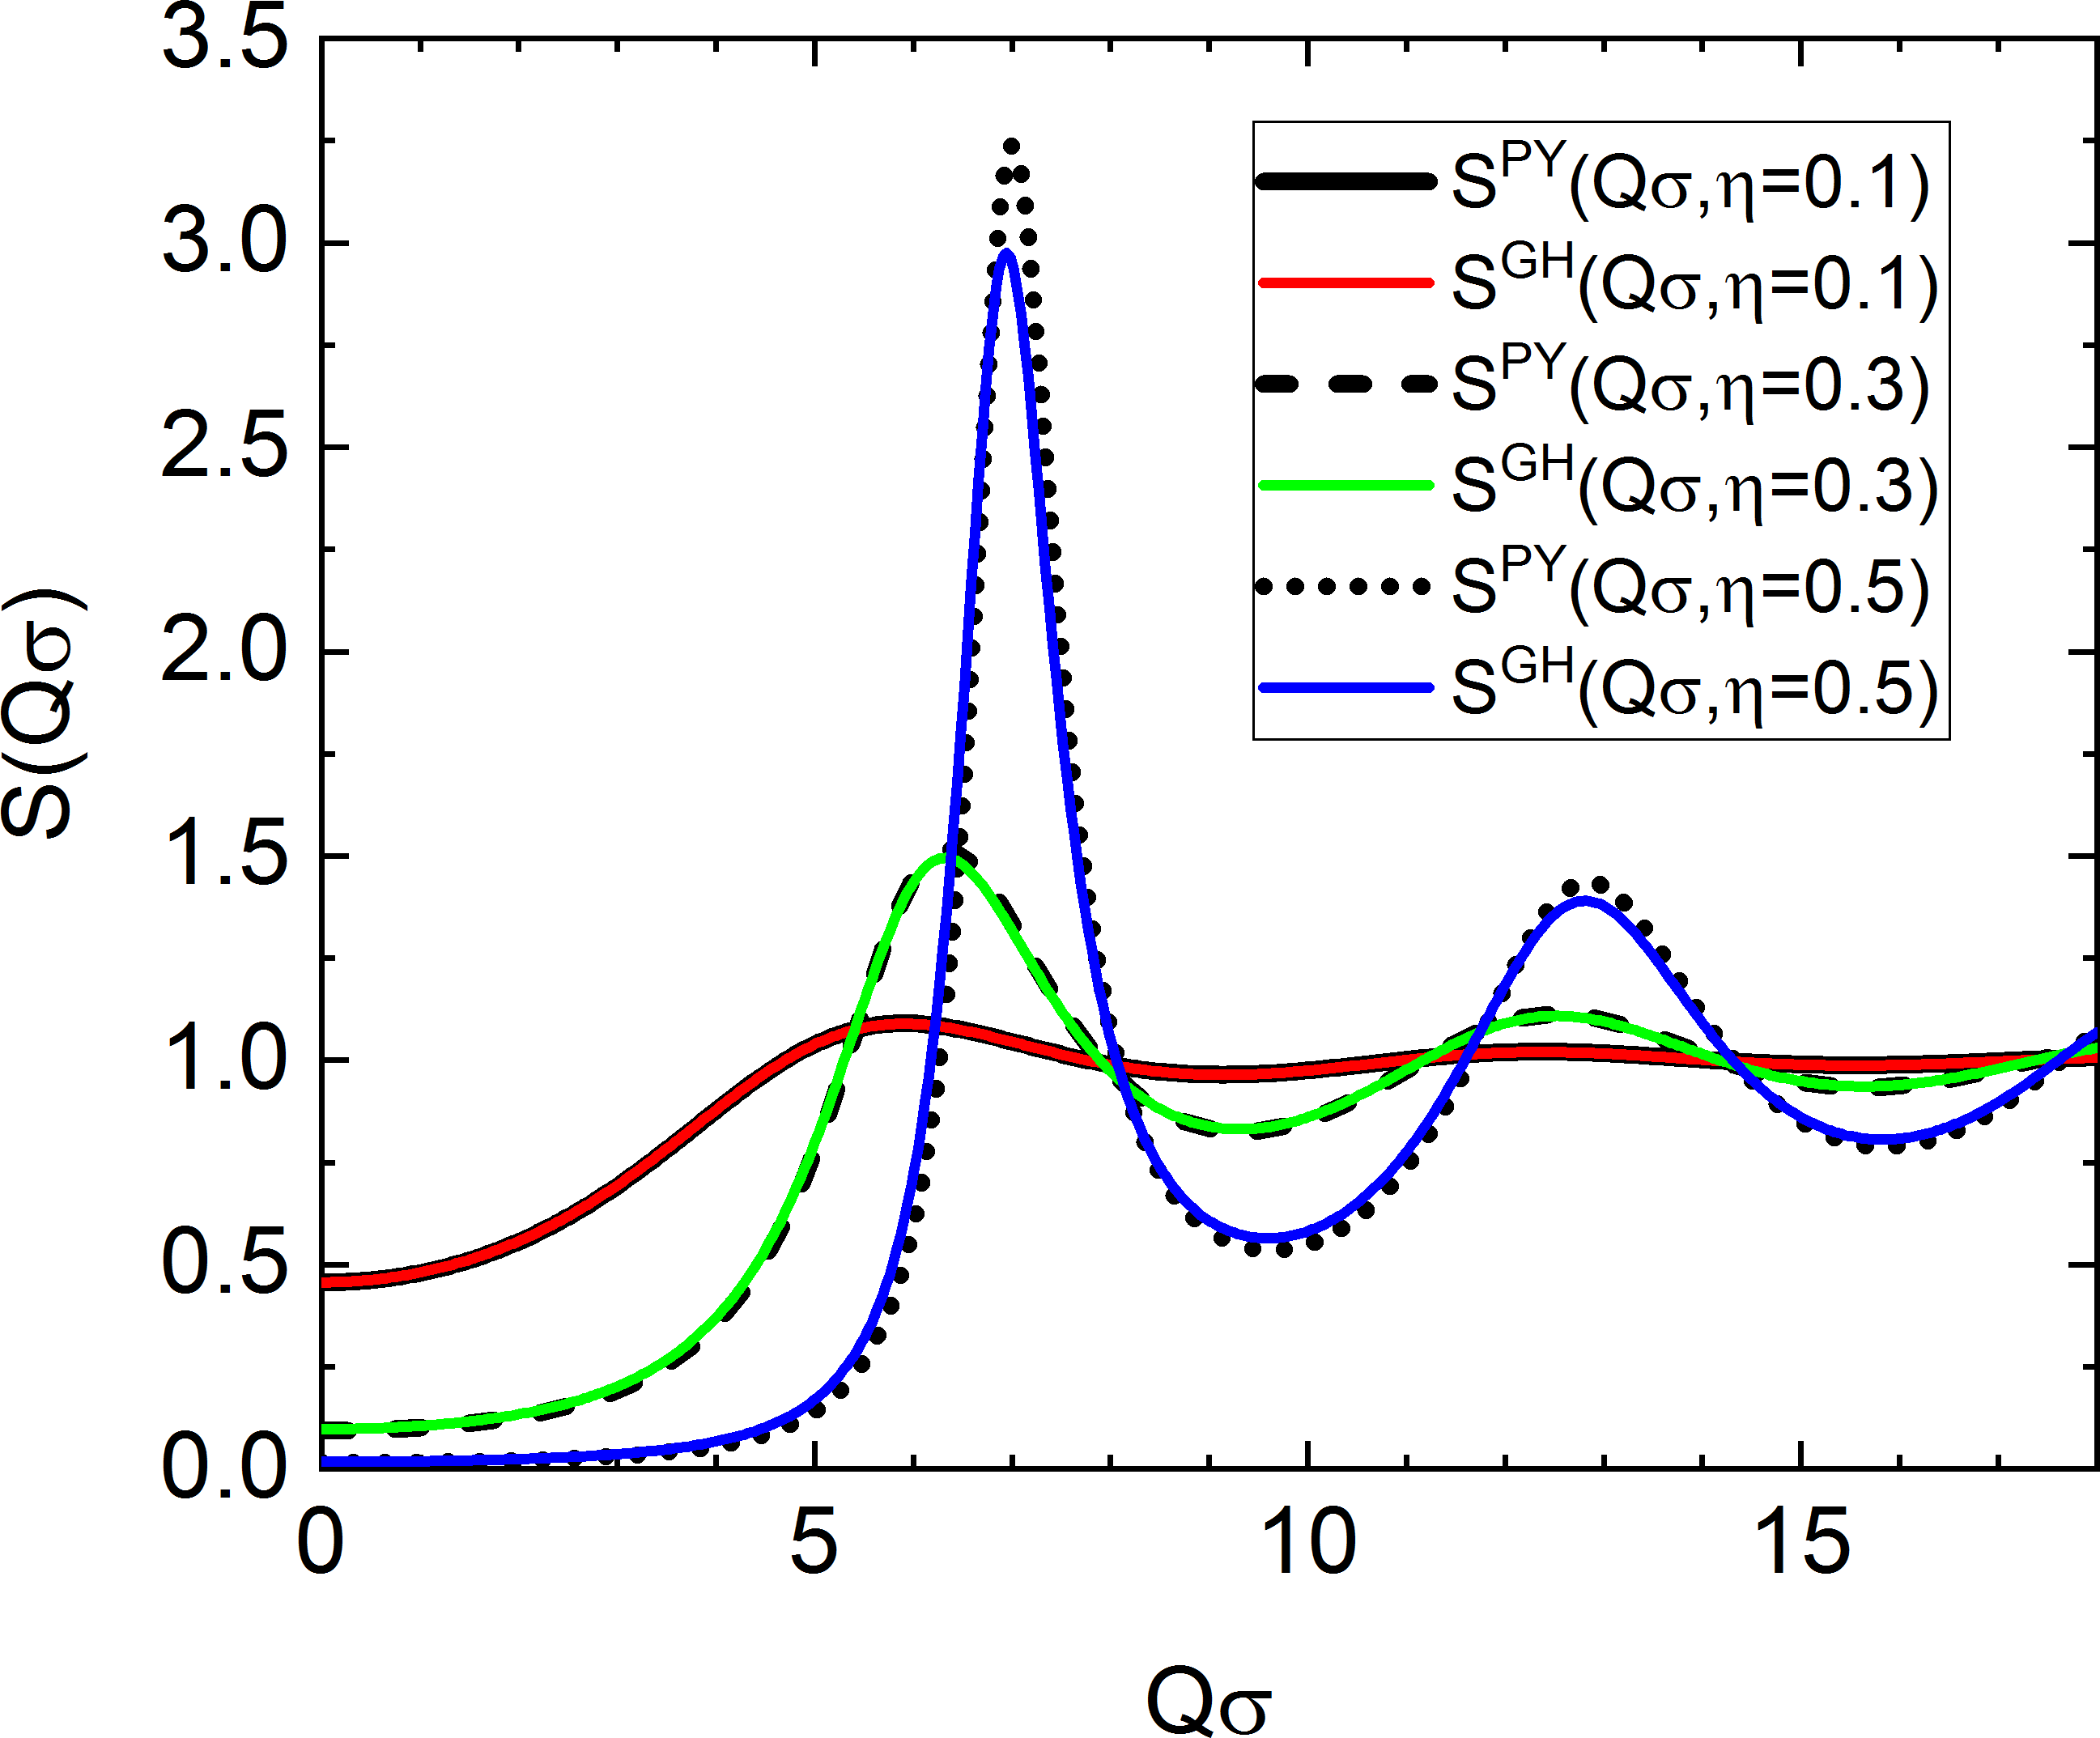
\includegraphics[width=0.46\textwidth]{../images/structure_factor/HardSphere/SQGH.png}}
\hfill
\subfigure[residual between $S^\mathrm{PY}$ and $S^\mathrm{GH}$]{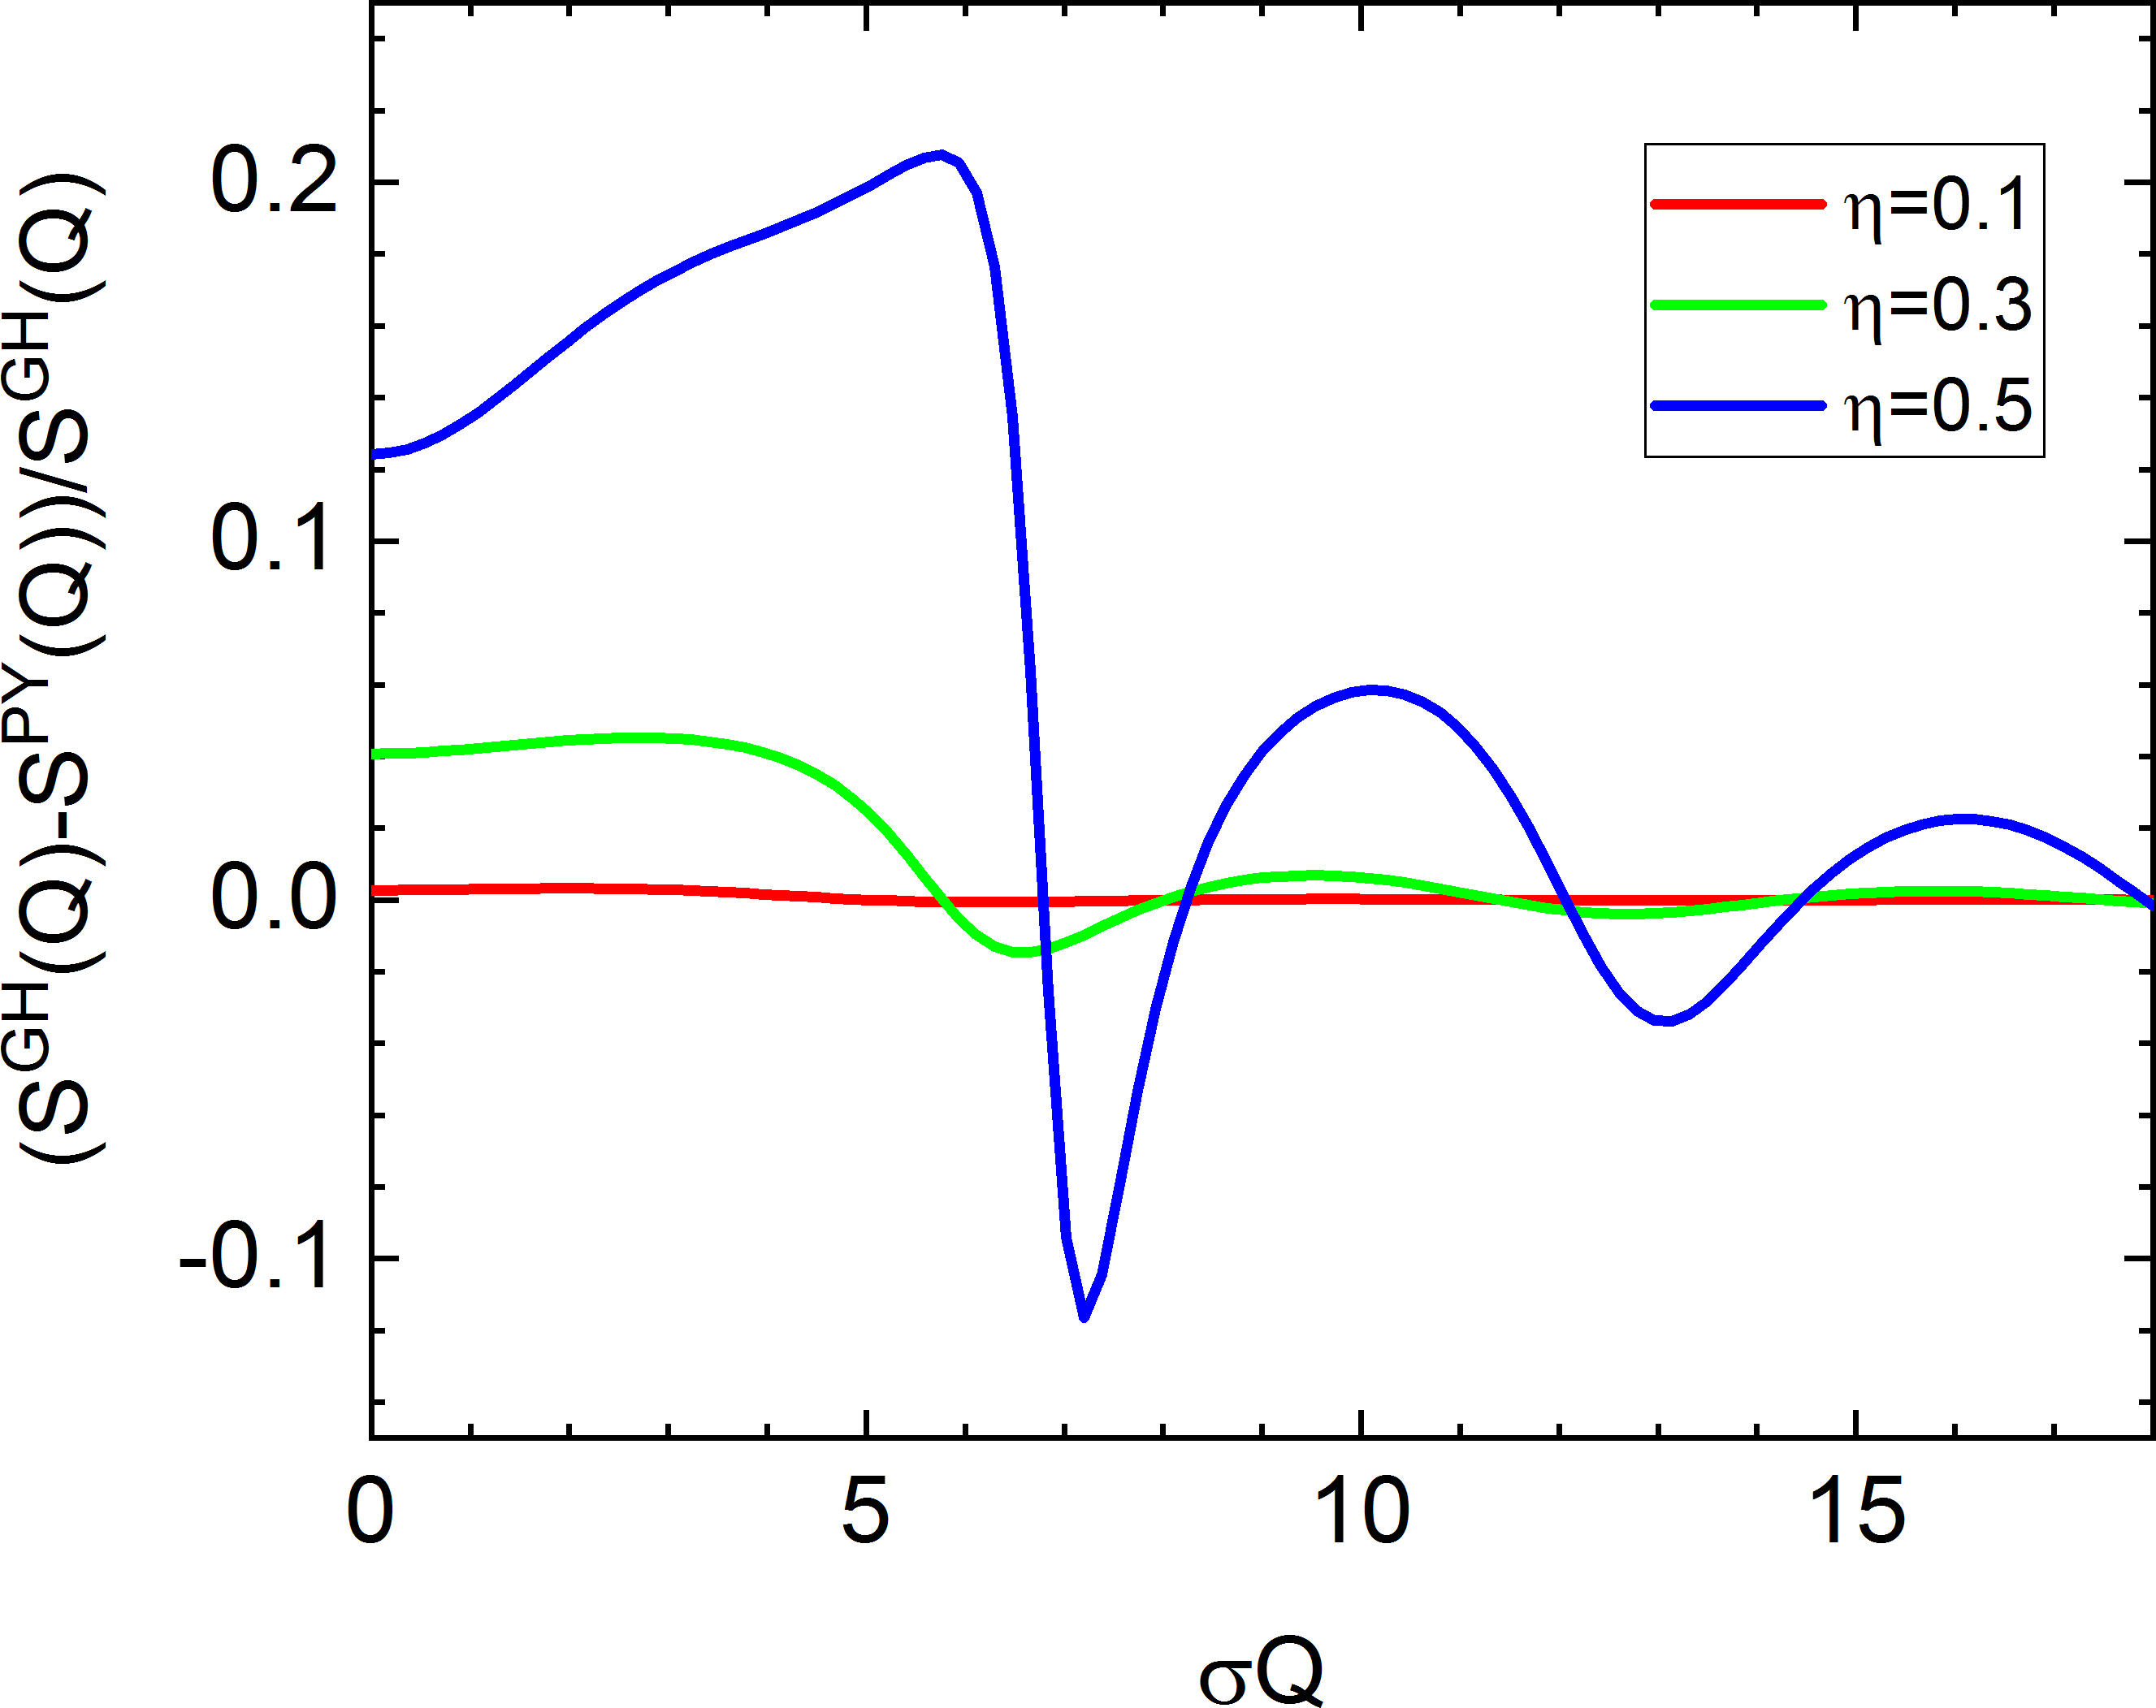
\includegraphics[width=0.48\textwidth]{../images/structure_factor/HardSphere/ResGH.png}} \\
\caption{Comparison between analytical PY solution of hard sphere static structure factor and thermodynamically consistent correction as described by Henderson and Grundke}
\label{fig:SQ:GH}
\end{figure}

\clearpage
\subsection{Hard Sphere (PY)} ~\\

\noindent This is the classical analytical solution of the Percus-Yevick equations \cite{Percus1958,Wertheim1963,Vrij1979} for a hard sphere potential
\begin{equation}
U(r) =
 \begin{cases}
      \infty    & \text{for} \quad 0<r<2R \\
      0         & \text{for} \quad r>2R
   \end{cases}
\end{equation}
The structure factor $S^\mathrm{PY}(Q)$ can be calculated 
\begin{subequations}
\begin{align}
\alpha &= \frac{\left(1+2\eta\right)^2}{\left(1-\eta\right)^4} \\
\beta  &= -6 \eta \frac{\left(1 +\eta/2 \right)^2}{\left(1-\eta\right)^4} \\
\gamma &= \frac{\eta \alpha}{2}  \\
A &= 2 R Q
\end{align}

\begin{align}
G(\eta,A) =  & \, \alpha \, \frac{\sin A -A \cos A }{A^2} + \beta \, \frac{2 A \sin A +(2-A^2) \cos A -2}{A^3} + \nonumber \\
    & \, \gamma  \, \frac{-A^4 \cos A + 4\left[(3A^2-6)\cos A+(A^3-6A)\sin A+6\right]}{A^5}
\end{align}
\begin{align}
S^\mathrm{PY}(Q,R,\eta)  = & \cfrac{1}{1+24 \eta
\cfrac{G(\eta,A)}{A}}
\end{align}
\end{subequations}

\vspace{5mm}

\hspace{1pt}\\
\underline{Input parameters for \texttt{Hard Sphere (PY)}:}
\begin{description}
    \item[\texttt{R}]  radius $R$
    \item[\texttt{eta}] volume fraction $\eta$
\end{description}

\noindent
\underline{Note}
\begin{itemize}
\item The structure factor accepts volume fractions between $\eta \in [0,1]$.
\end{itemize}

\begin{figure}[htb]
\begin{center}
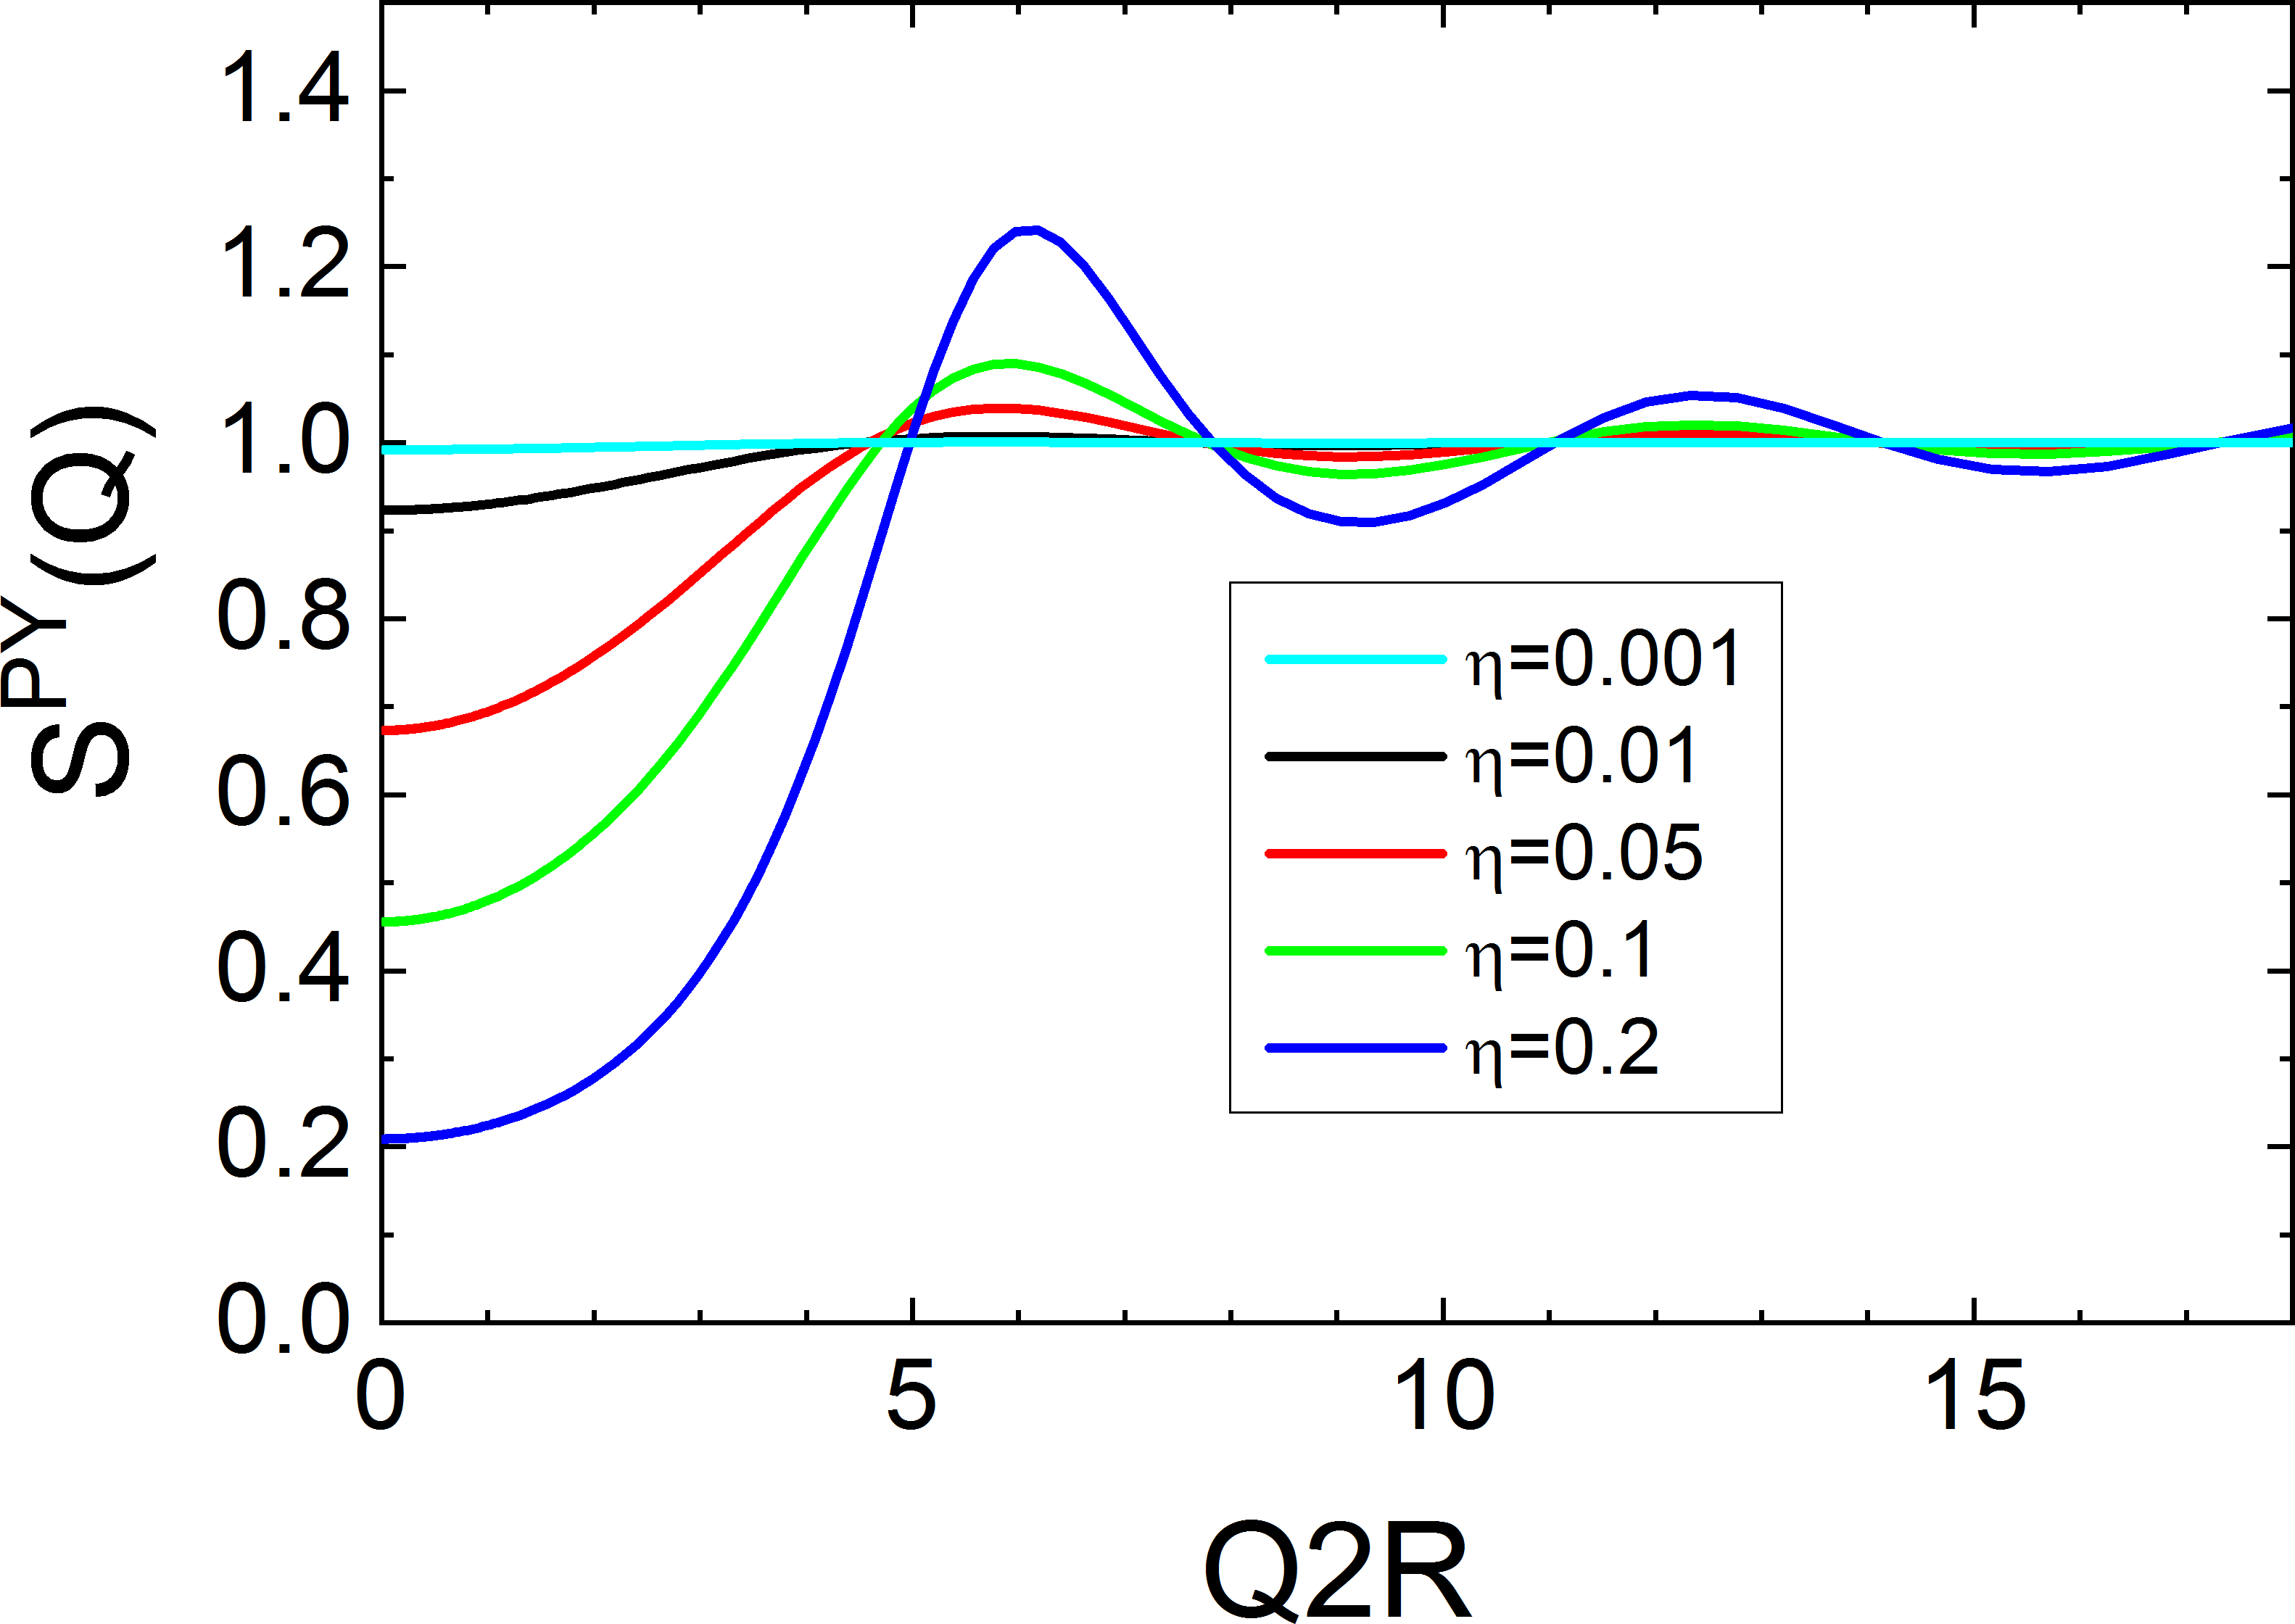
\includegraphics[width=0.6\textwidth]{../images/structure_factor/HardSphere/SQPY.png}
\end{center}
\caption{Structure factor $S^\mathrm{PY}(Q)$ for a hard sphere interaction potential for the different volume fractions $\eta$.}
\label{fig:SQPYHardSphere}
\end{figure}

\clearpage
\section{Structure factor for a two dimensional hard spheres/disks fluid} \hspace{1pt}
The structure factor of hard disks or spheres with diameter/radius $\sigma=2R$ in two dimensions with an interaction potential
\begin{align}
U(r,\sigma) &=
\begin{cases}
\infty &\mathrm{for~}  r < \sigma \\
0  &\mathrm{for~}  r \geq \sigma
\end{cases}
\end{align}
have been implemented in several variants.
An analytical form of the structure factor as a function of the disk radius $R$ and surface coverage $\eta=\pi R^2 \rho$, where $\rho$ is the number density of particles, have been given by\cite{Rosenfeld1990,Guo2006}.
Rosenfeld \cite{Rosenfeld1990} gives the expression
\begin{align}
\frac{1}{S(q)}-1 &= 4\eta\left(A \frac{\mathrm{J}_1^2(qR)}{(qR)^2}
                    +B\mathrm{J}_0(qR)\frac{\mathrm{J}_1(qR)}{qR}
                    +G\frac{\mathrm{J}_1(2qR)}{qR}
                    \right)
\end{align}
with
\begin{align}
A &=\left(1+(2\eta-1)\chi+2\eta G\right)/\eta \\
B &=\left((1-\eta)\chi-1-3\eta G\right)/\eta \\
G &= \frac{1}{1-\eta} \\
\chi &= \frac{1+\eta}{(1-\eta)^2}
\end{align}
In the original paper from Rosenfeld the definition of $\chi$ seems to have a typo and has been corrected like in \cite{Engel2009}.
Guo \cite{Guo2006} supplies the expression
\begin{align}
S(q) &= \frac{1}{1-\rho \tilde{c}(q,r)} \\
\tilde{c}(q,r) &= 2\pi\sigma^2 \int_0^1 c(r′,\eta) J_0(q\sigma r′) r′ \mathrm{d}r′
\end{align}
with
\begin{align}
\begin{split}
c(r',\eta) &=
\Theta(1-r') \left[-\frac{1-p\eta^2}{\left(1-2\eta+p\eta^2\right)^2}\right]  \\
&\left\{1-a^2\eta-a^2\eta\frac{2}{\pi}\left[\arccos\left(\frac{r'}{a}\right)-\frac{r'}{a}\sqrt{1-\frac{r'^2}{a^2}}\right]\right\}
\end{split}
\end{align}
with $p=\left(4\sqrt{3}\pi-12\right)/\pi^2$ and $\Theta()$ being the Heaviside function. The parameter $a$ is the root of a non-linear equation, which has been solved numerically and then approximated via a polynomial fitting by
\begin{align}
a &= 0.3699\eta^4
      -1.2511\eta^3
      +2.0199\eta^2
      -2.2373\eta
      +2.1
\end{align}

\vspace{5mm}
\noindent
\underline{Input Parameters for model \texttt{2D hard disks (Rosenfeld)} as well as}
\underline{\texttt{2D hard disks (Guo)}:}\\
\begin{description}
\item[\texttt{R}] radius of the disc $R$
\item[\texttt{eta}] surface coverage $\eta$
\end{description}


\noindent\underline{Note:}
\begin{itemize}
\item Both models break down for surface coverage around $\eta>0.75$. The densest possible lattice packing would be $\eta_\mathrm{max}=\frac16\pi\sqrt{3}\simeq 0.907$.
\item Values for surface coverage $0 < \eta < 1$ are accepted by the software.
\end{itemize}

\begin{figure}[htb]
\centering
  \subfigure[]{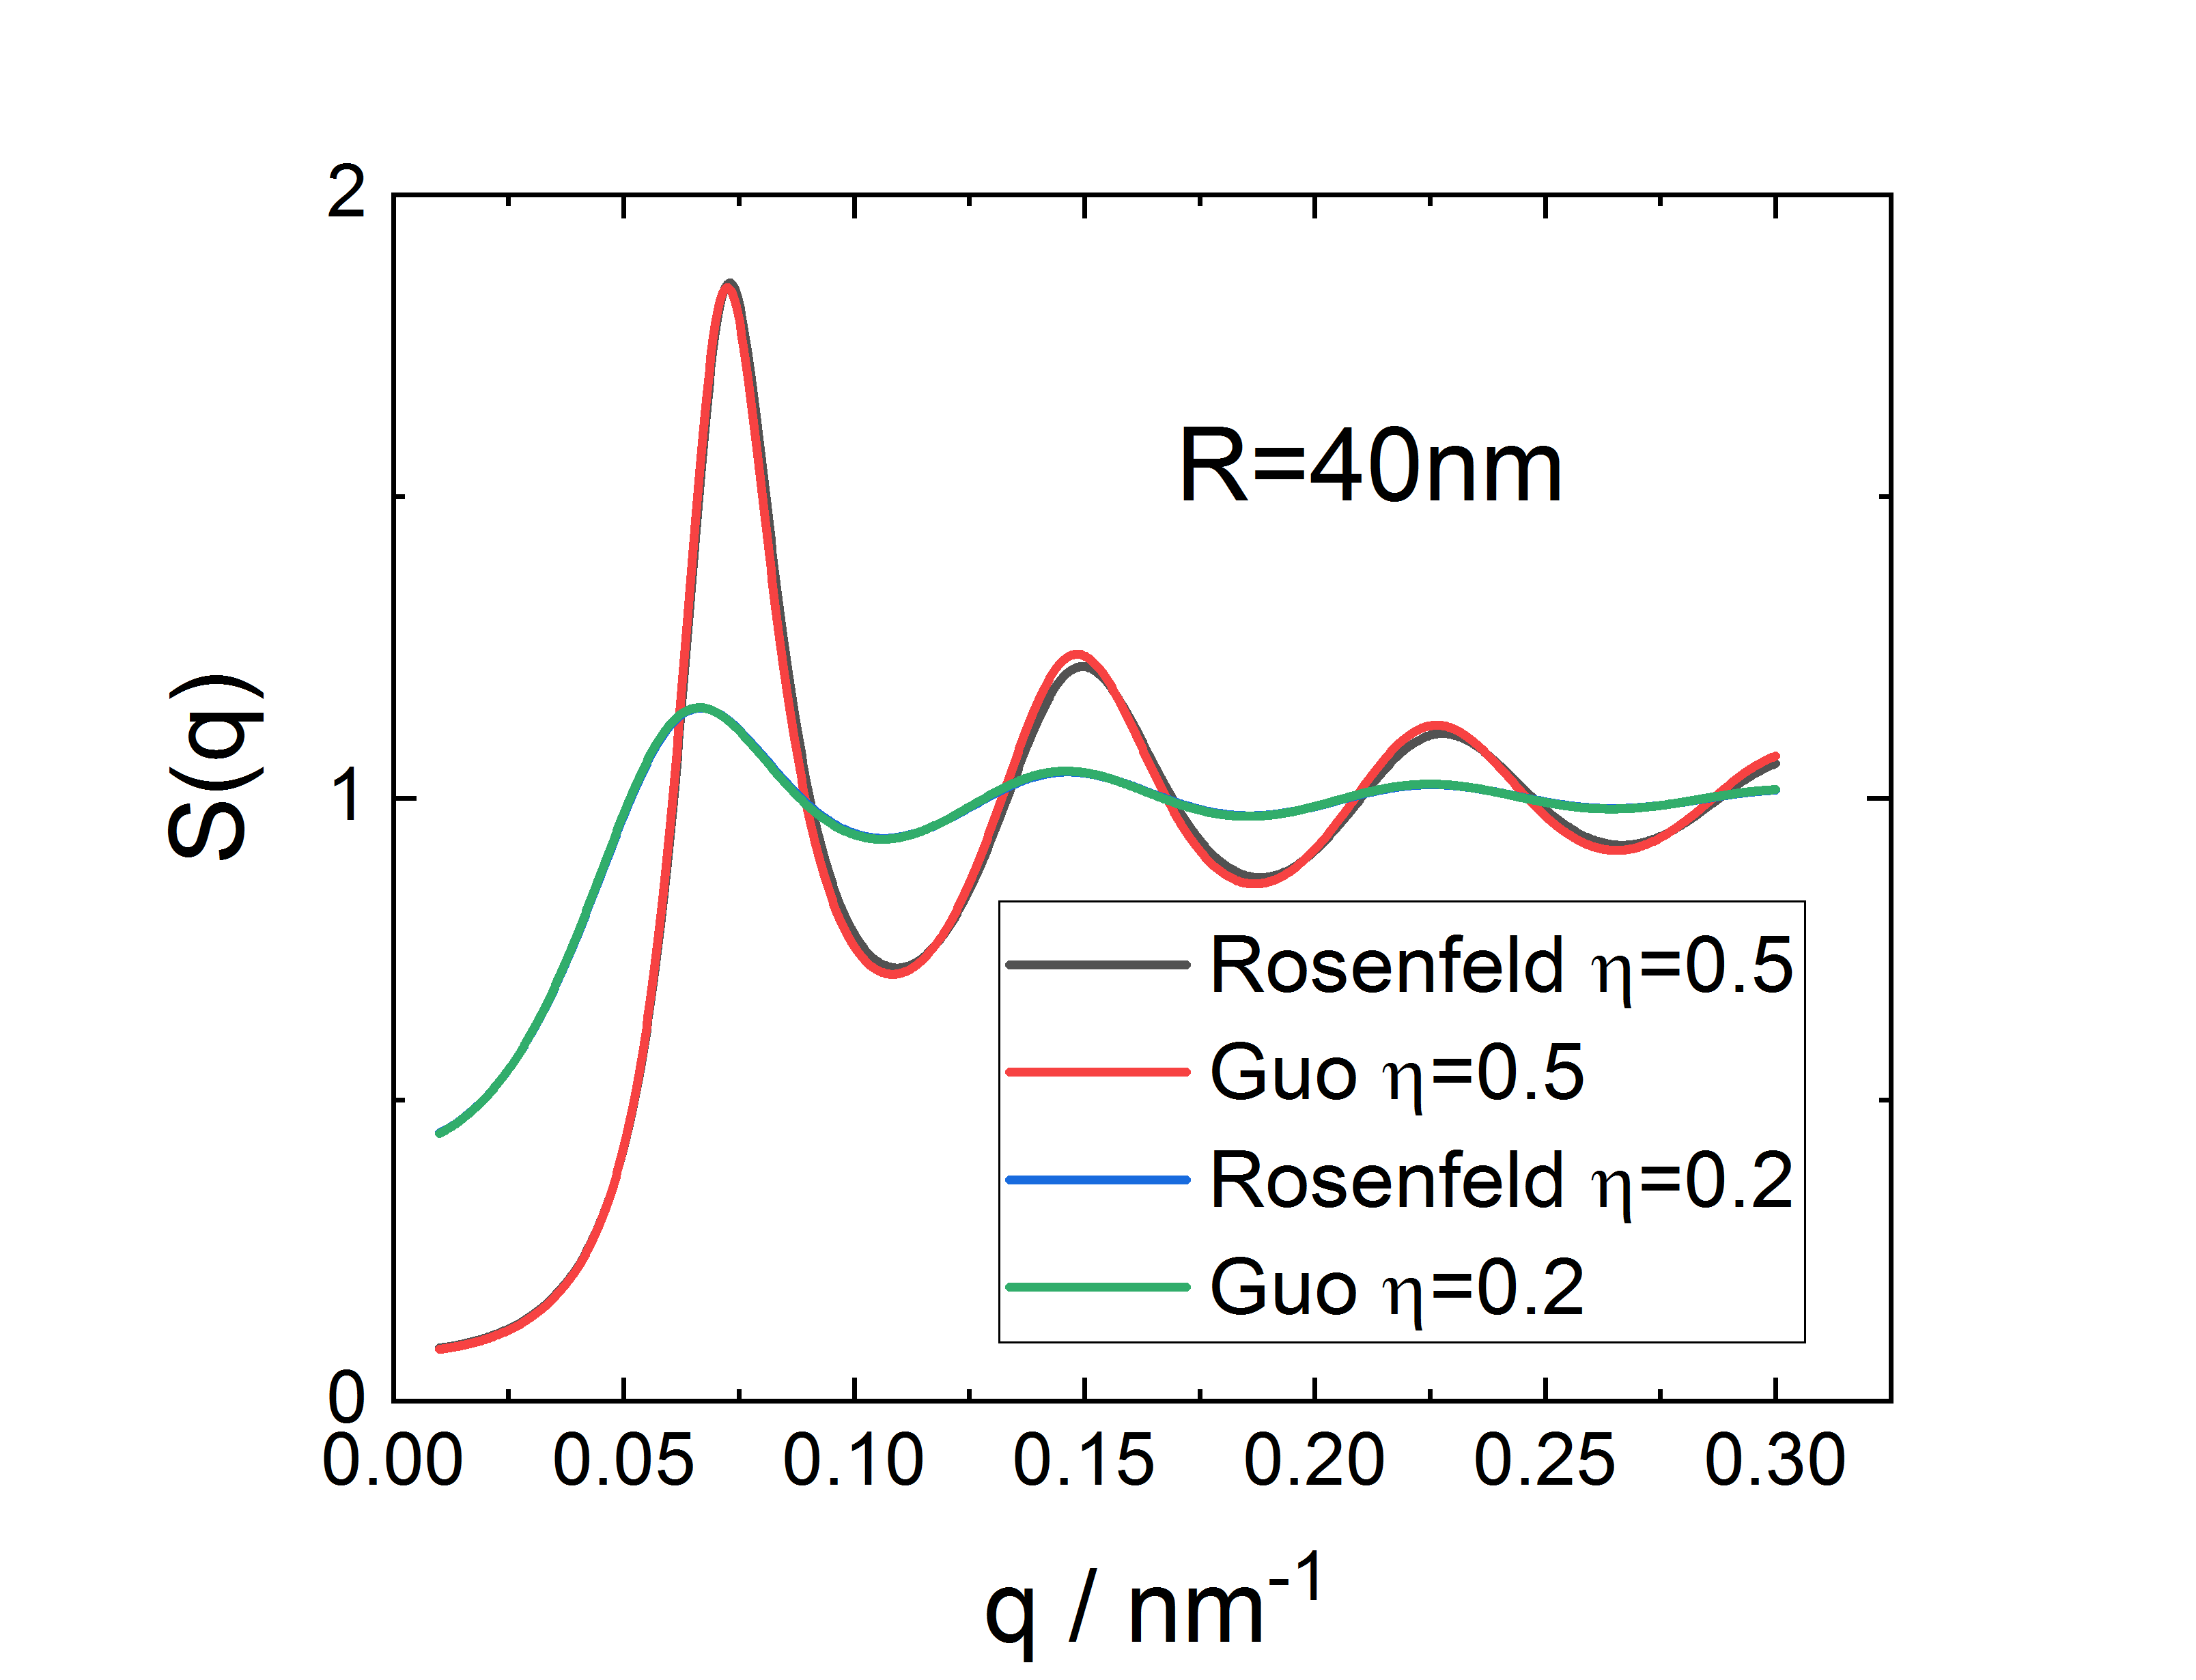
\includegraphics[width=0.43\textwidth]{../images/structure_factor/2D_hard_disk_fluid/HardDisks_low.png}}
  \quad
  \subfigure[]{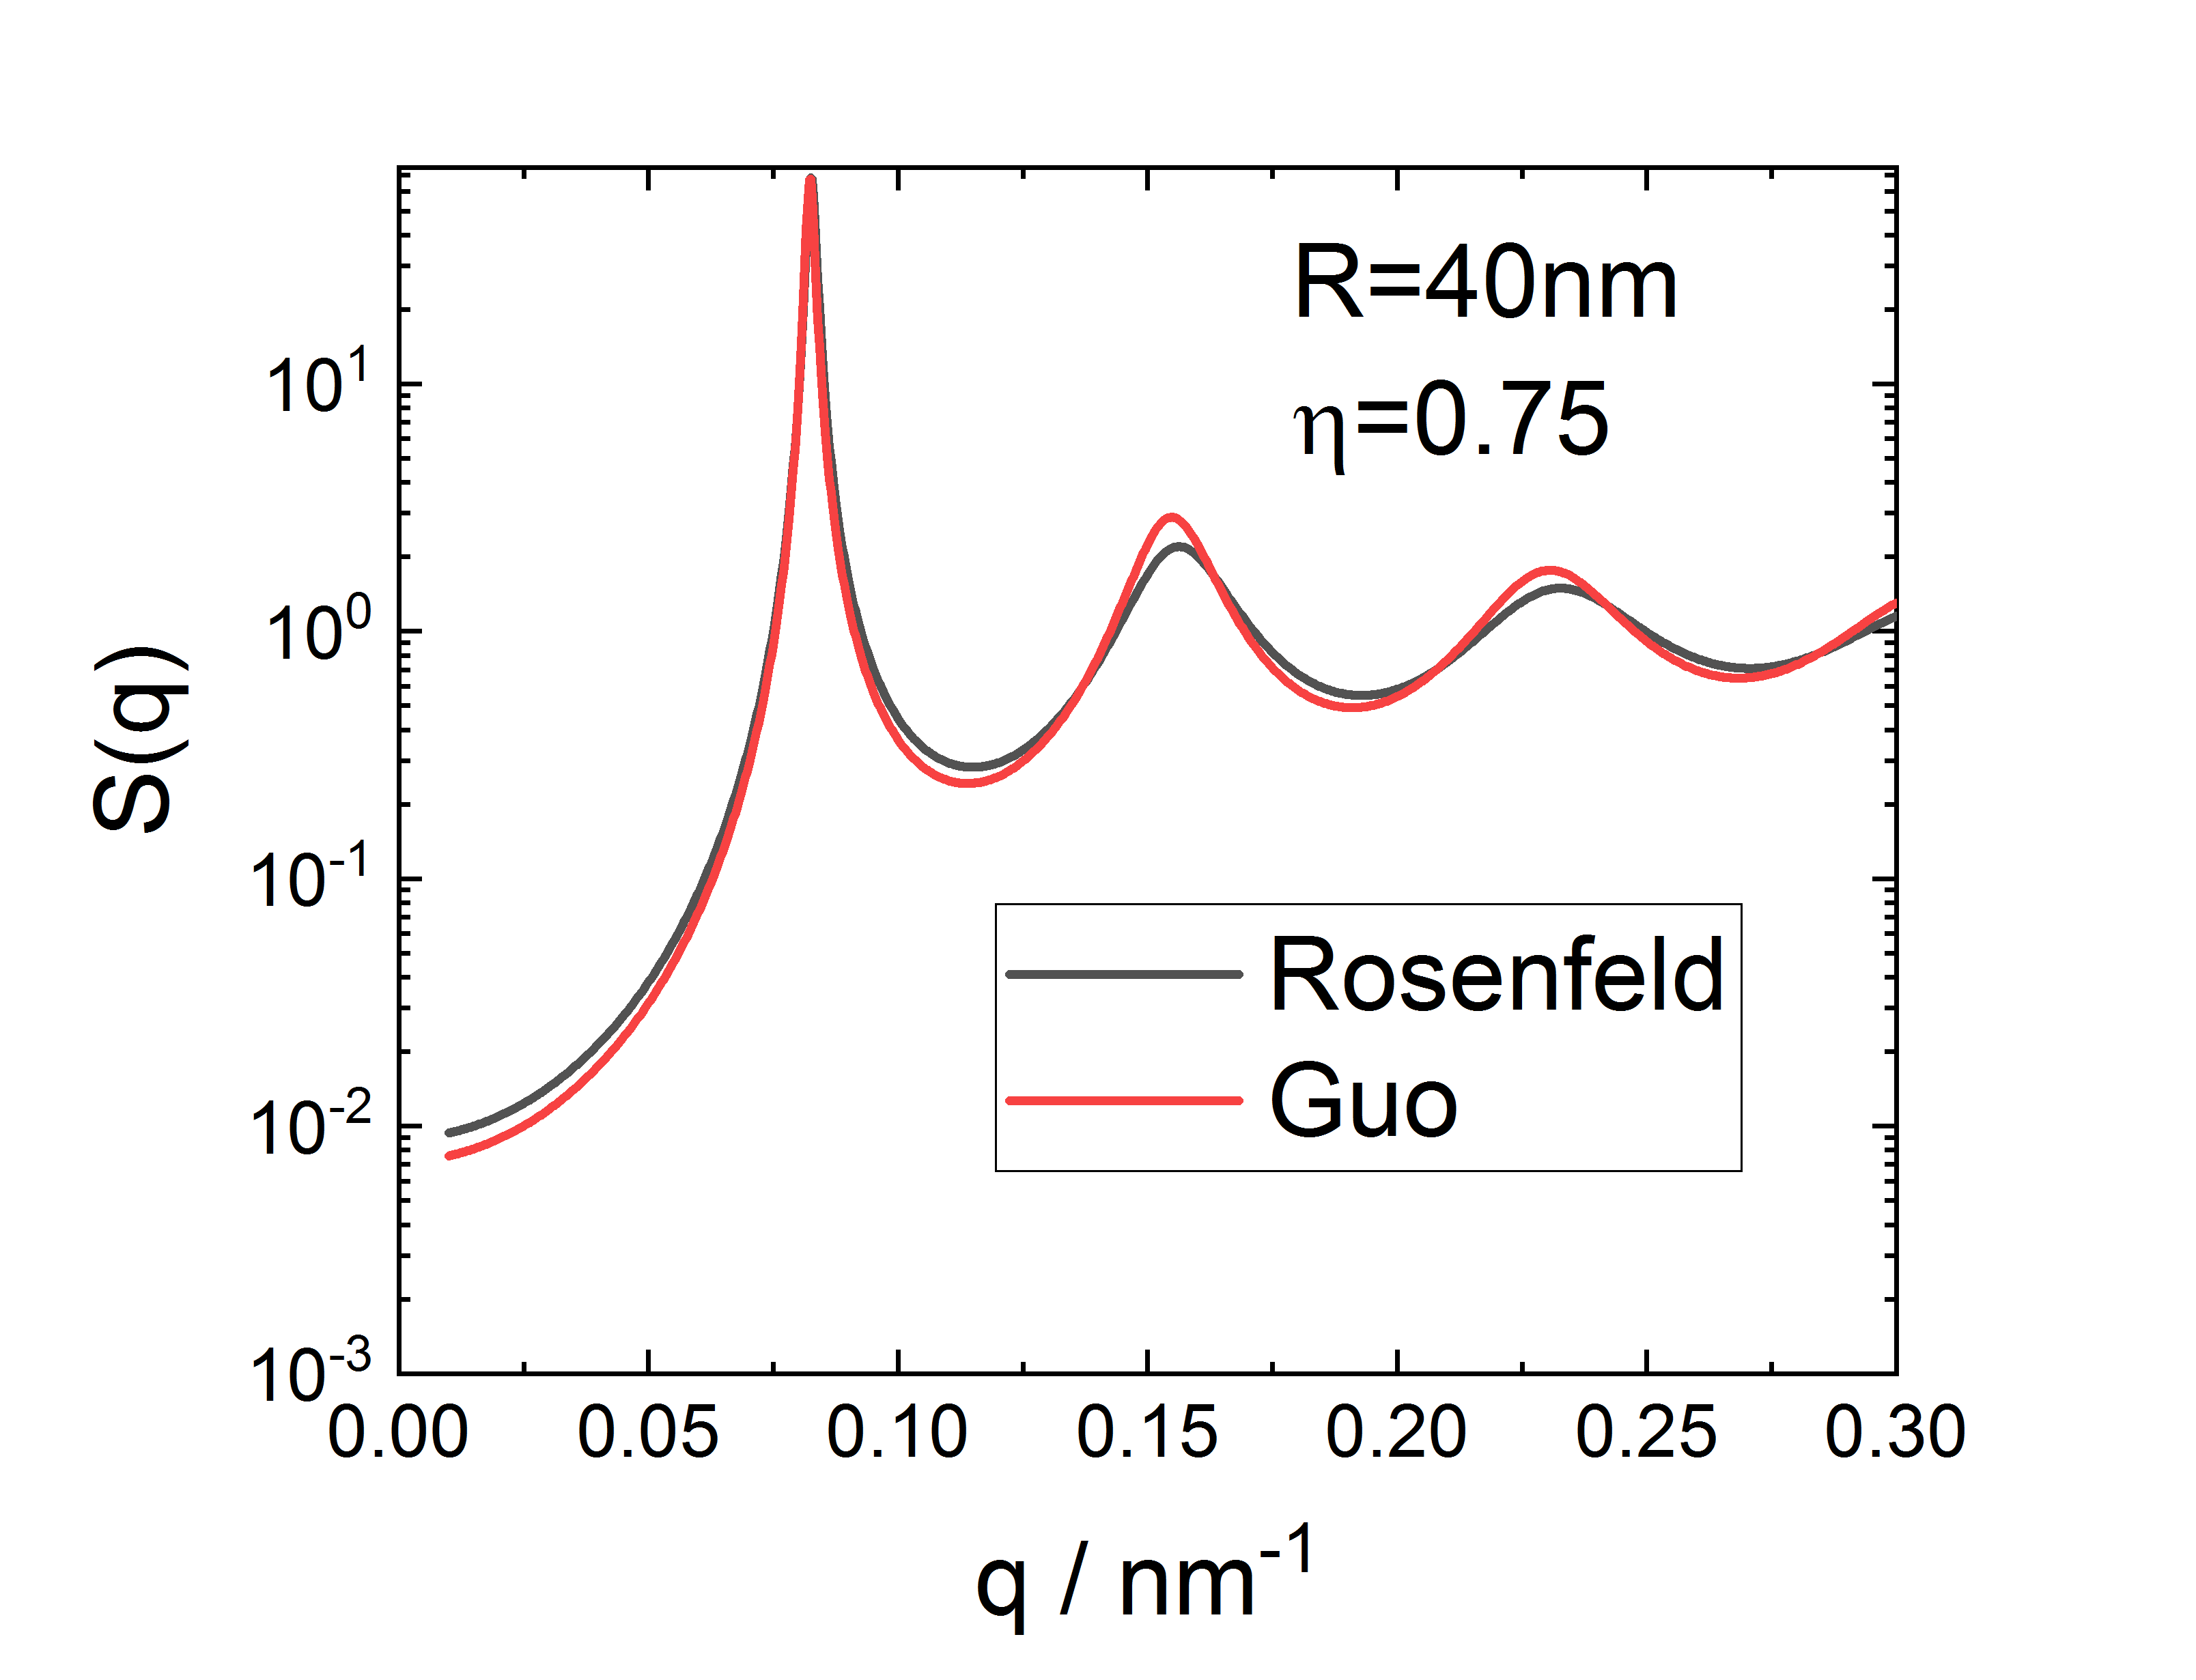
\includegraphics[width=0.47\textwidth]{../images/structure_factor/2D_hard_disk_fluid/HardDisks_high.png}}
  \caption{Comparison between Rosenfeld's and Guo's results}
\end{figure}

%%%%%%%%%%%%%%%%%%%%%%%%%%%%%%%%%%%%%%%%%%%%%%%%%%%%%%%%%%%%%%%%%%%%%%%%%%%%%%%%%%%%%%%%
\section{Structure factor of a random flight model} \hspace{1pt}
The random flight model describes a discrete chain, where the positions of the $N$ units forming the discrete chains follow a 3D random walk. The distance between neighbouring units is constants.
\begin{figure}[htb]
\begin{center}
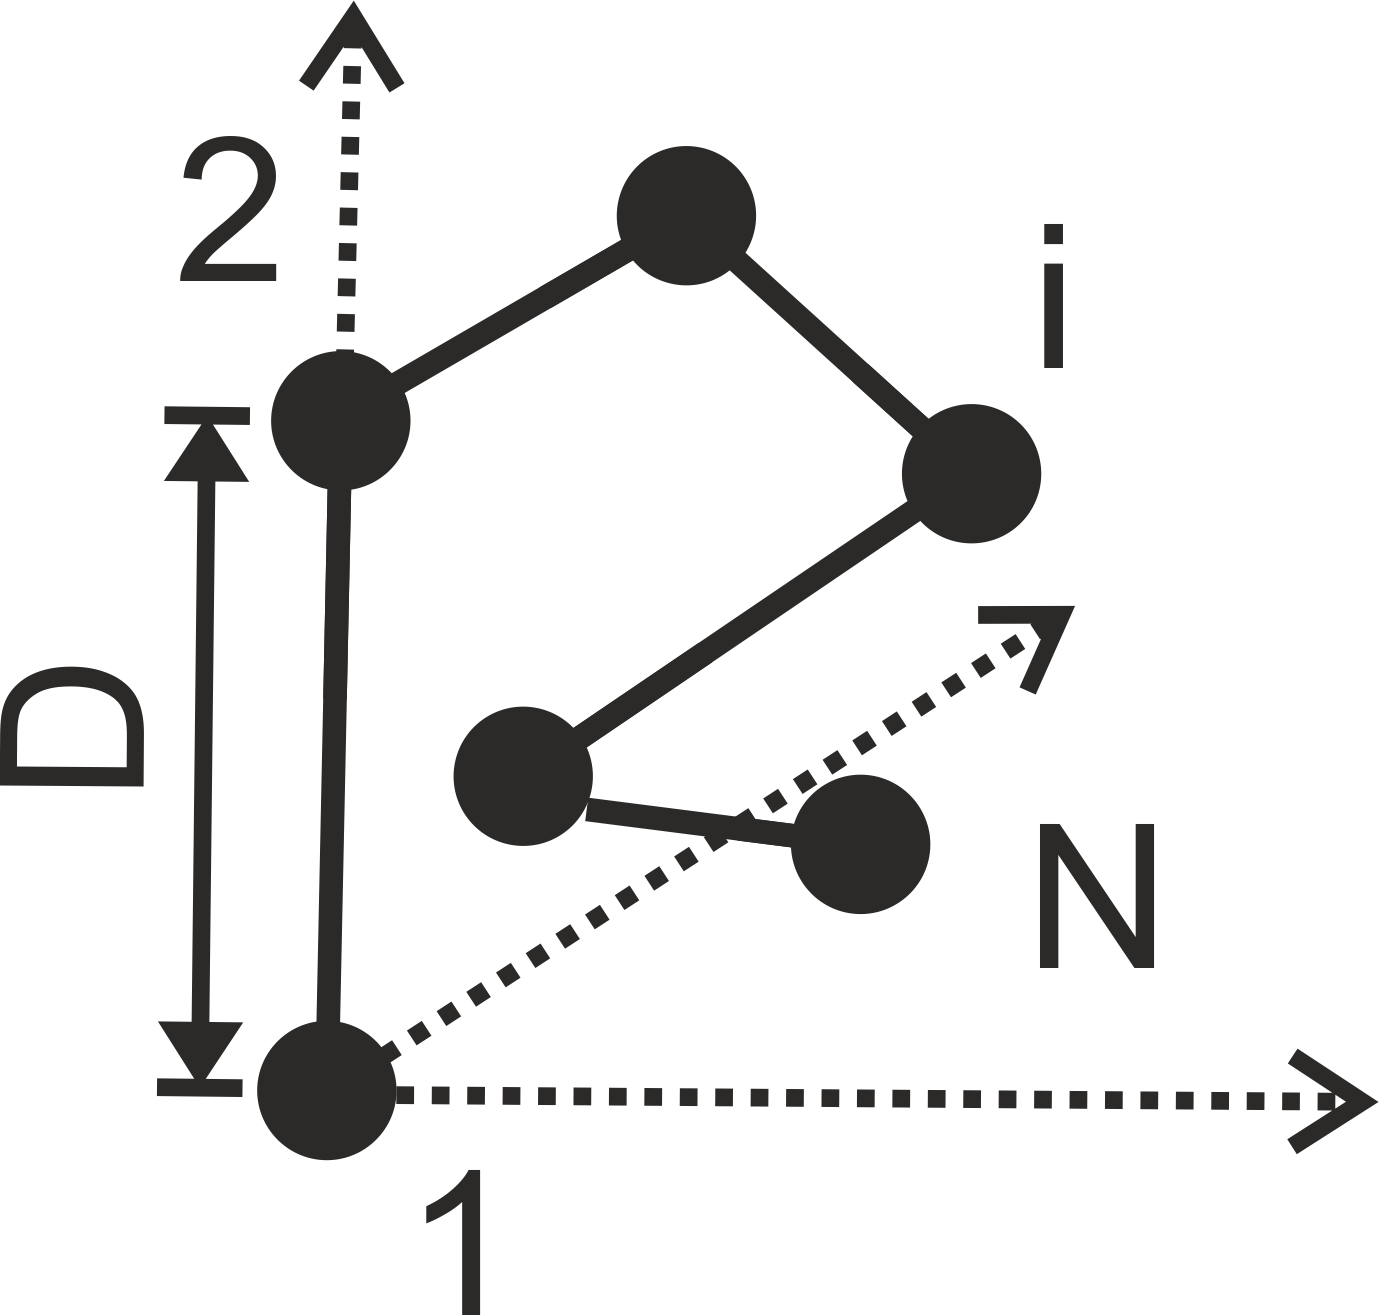
\includegraphics[width=0.35\textwidth]{../images/structure_factor/randomflight3D.png}
\end{center}
\caption{Random flight of $N$ particles with constant distances $D$.}
\label{fig:randomflight3D}
\end{figure}
The structure factor $S_N(QD)$ describing such an arrangement of $N$ particles on a random flight
with a constant step size $D$ is given by \cite{Burchard1970} as
\begin{align}
S_N(QD)&=
     \frac{2}{1-\frac{\sin⁡(QD)}{QD} )}-1-\frac{2\left[1-\left[\frac{\sin⁡(QD)}{QD}\right]^N \right]}{N\left[1-\frac{\sin⁡(QD)}{QD}\right]^2}   \frac{\sin⁡(QD)}{QD}
\end{align}
The formula above is only real for all values of $QD$ for integer values of $N$. For non integer values $N$ a linear interpolation between $[N]$ and $[N]+1$ is taken \cite{Giehm2010}, where $[N]$ is the largest integer smaller or equal to $N$. With $w=N-[N]$ we get
\begin{align}
S_N(QD)&= (1-w)S_{[N]}(QD) + wS_{[N]+1}(QD)
\end{align}

\noindent \underline{Input Parameters for model \texttt{random flight}:}\\
\begin{description}
\item[\texttt{D}] step length $D$
\item[\texttt{n}] number of steps $N$
\end{description}


\noindent\underline{Note:}
\begin{itemize}
\item $N$ needs to be larger or equal to 1. For non-integer values of $N$ the curve is linear interpolated between the structure factor for $N$ and $N+1$.
\end{itemize}

\begin{figure}[htb]
\begin{center}
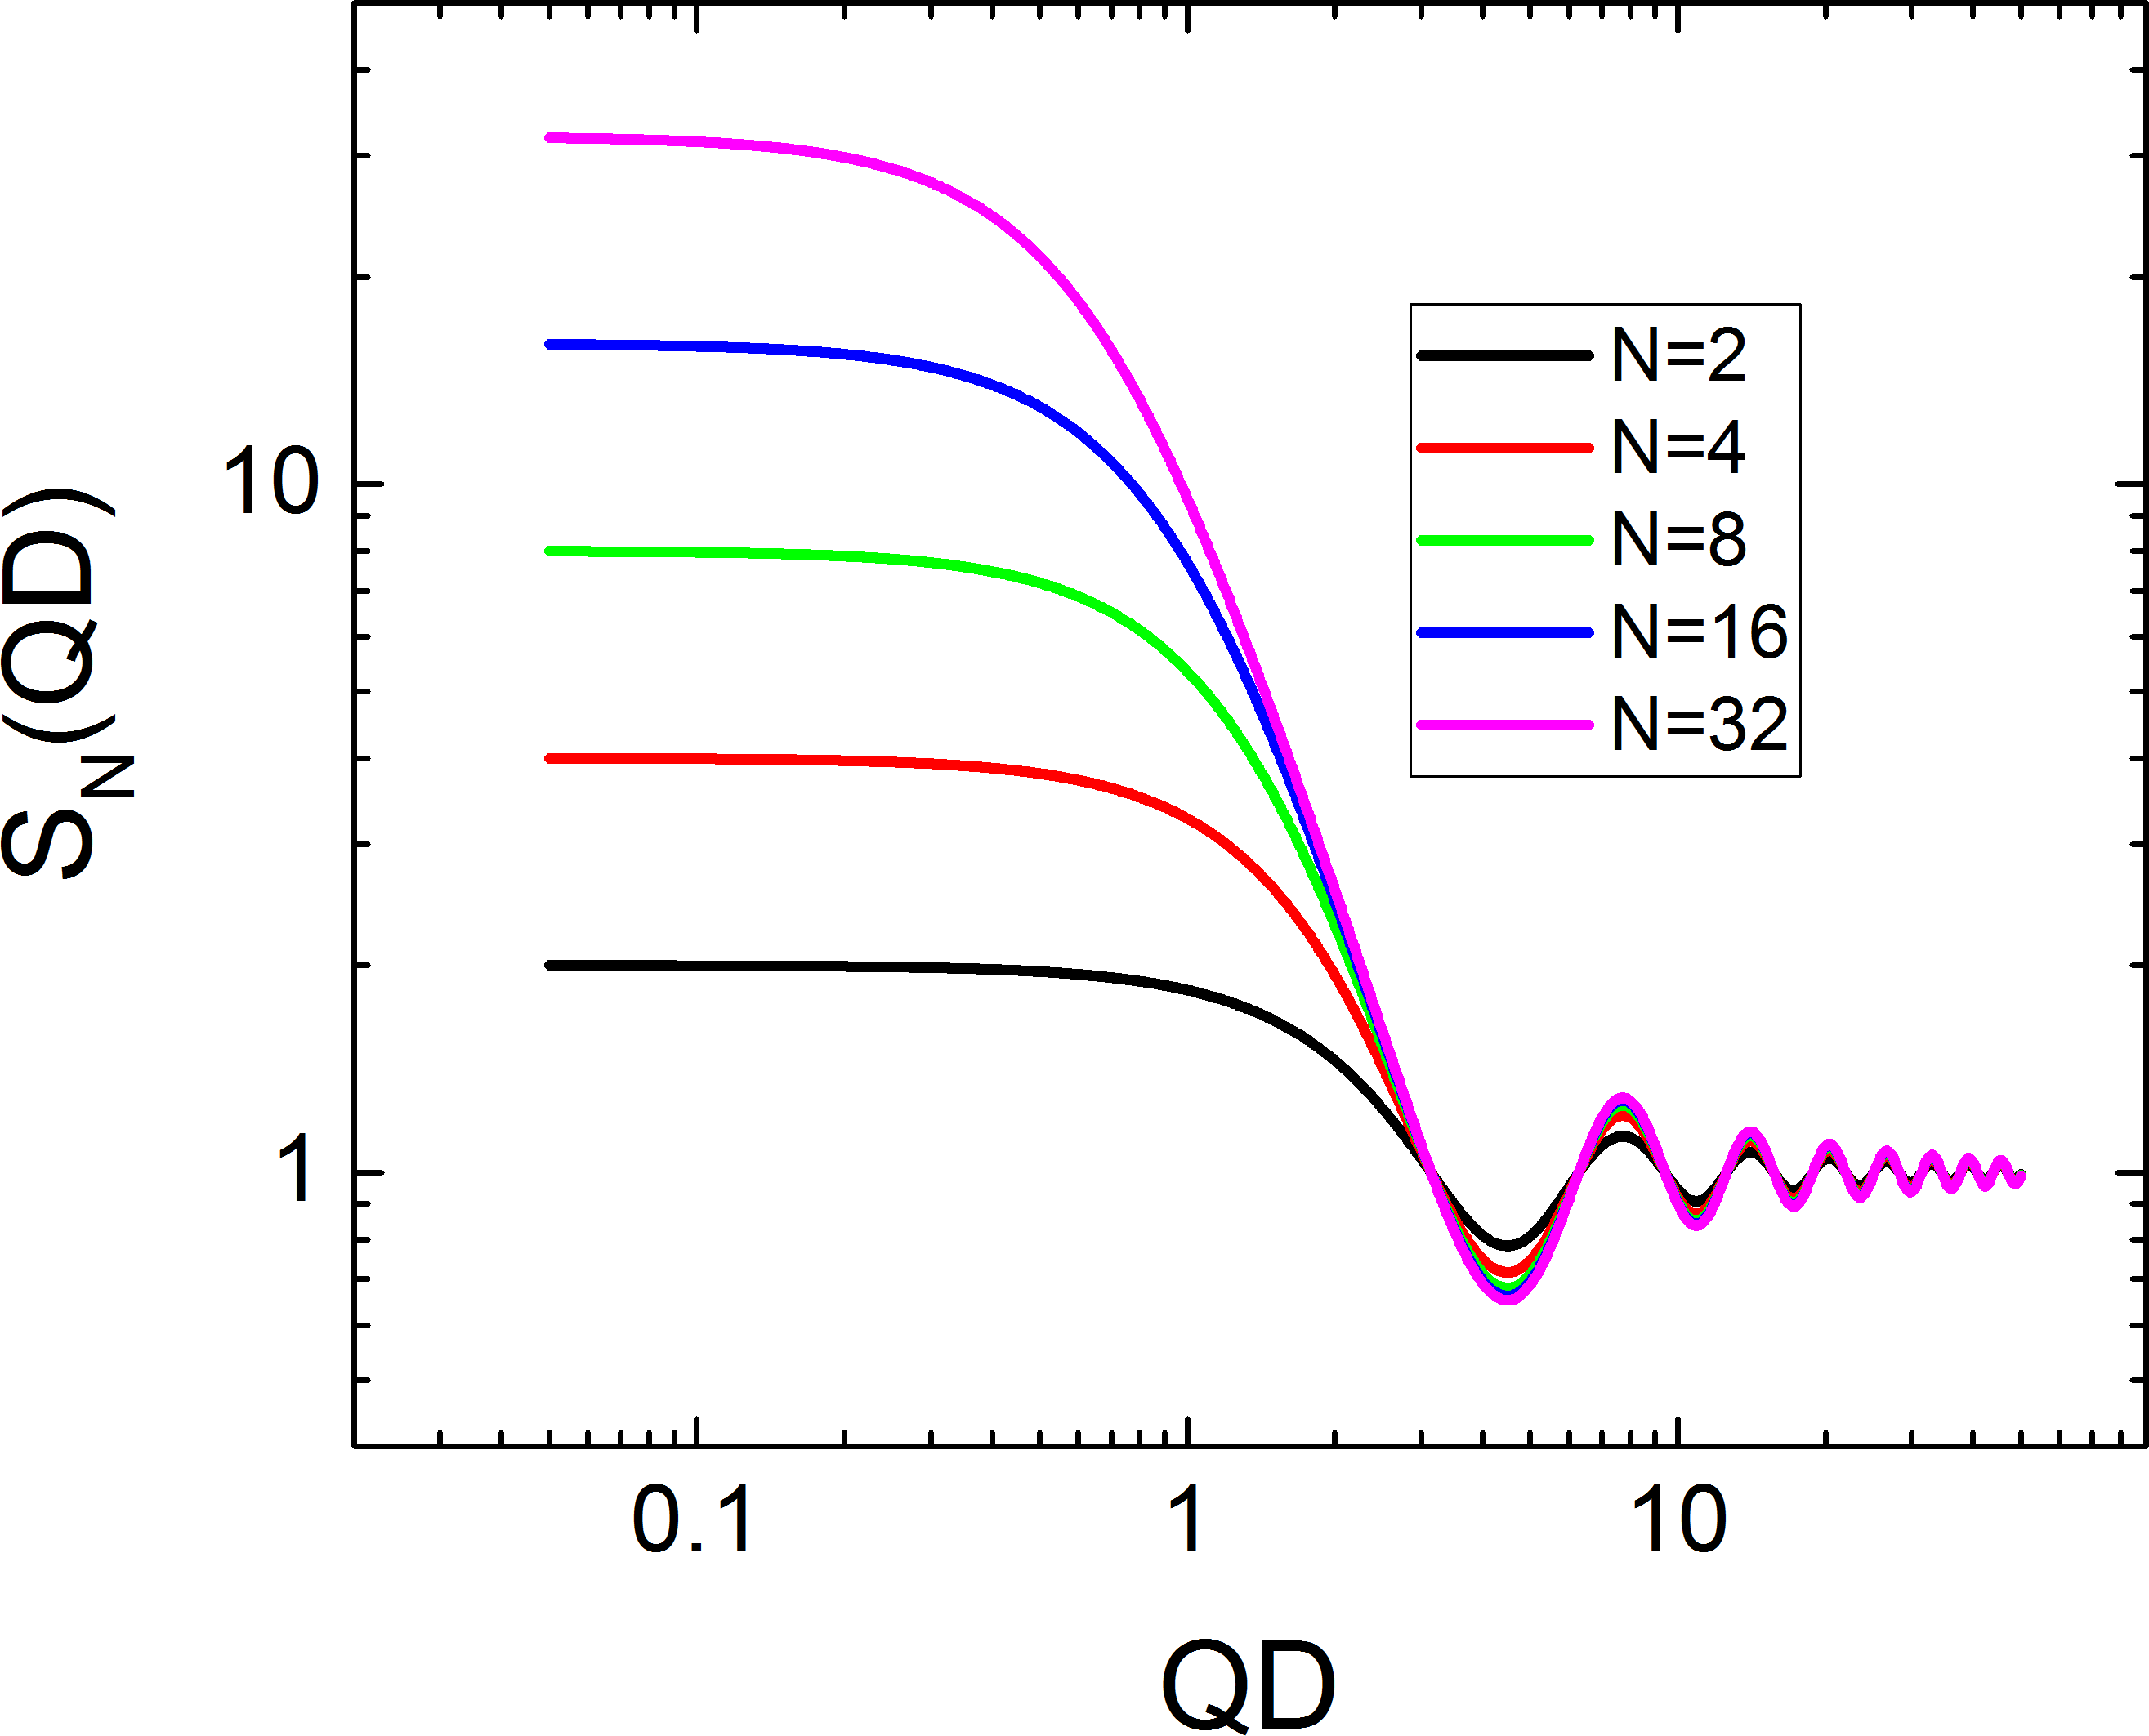
\includegraphics[width=0.75\textwidth]{../images/structure_factor/randomflight.png}
\end{center}
\caption{Random flight structure factor with $N$ steps of length $D$.}
\label{fig:randomflight}
\end{figure}

%%%%%%%%%%%%%%%%%%%%%%%%%%%%%%%%%%%%%%%%%%%%%%%%%%%%%%%%%%%%%%%%%%%%%%%%%%%%%%%%%%%%%%%%
\section{ordered particle systems} \hspace{1pt}
\label{sec:ops}
This plugin contains the structure factor of ordered mesoscopic materials in case the domains are random orientated like in powder diffraction as described in \cite{Forster2005}. For oriented domains the scattering pattern is not anymore radial symmetric and depends both on the direction and modulus of the scattering vector. For this case the structure factor are taken from  \cite{Forster2011}. This plugin tries to re-implement the functions which are originally supplied by the software package \texttt{scatter} described in \cite{Forster2010}. The software package \texttt{scatter} is specialised on calculating and fitting ordered structures and has much more options and better GUI for this kind of studies. In both case the structure factor is approximated in the decoupling approach (\cite{Kotlarchyk1983}) as defined in \ref{sec:SQdecoupling} or in eq.\ \ref{Mittel} of section \ref{sec:decouplingGF}

In case of random oriented domains of three dimensional ordered particle systems the decoupling approach is implemented as
\begin{align}
I(Q) &= \langle\overline{F^2(Q)}\rangle_{or} + \langle\overline{F(Q)}\rangle_{or}^2 (S(Q)-1)
\end{align}
The overline symbol denotes the average over a particle size distribution and the brackets $\langle\rangle_{or}$ for the orientational average. In the above case it is assumed that the position of the scatterer is independent
of their size and orientation. For small size distributions and only small deviations from spherical symmetry of the scatterer the decoupling approximation works quite well.
For two and one dimensional ordered particle systems the particles can be very anisotropic, i.e.  very long cylindrical in case of 2D ordering and thin planar objects in case of 1D ordering. For this very anisotropic shaped particles the scattering amplitude and scattering intensity can be written as a product \ref{sec:very_anisotropic_particles} in terms of a cross section term for the short dimension $L_\mathrm{short}$ and a shape factor for the long dimension $L_\mathrm{long}$ as well as there averages
\begin{subequations}
\begin{align}
F(Q,L_\mathrm{short},L_\mathrm{long}) &= F_\mathrm{cs}(Q,L_\mathrm{short}) F'(Q,L_\mathrm{long}) \\
\langle\overline{F^2(Q,L_\mathrm{short},L_\mathrm{long})}\rangle_{or} &= \langle\overline{F^2_\mathrm{cs}(Q,L_\mathrm{short})}\rangle_{or} \langle\overline{F'^2(Q,L_\mathrm{long})}\rangle_{or} \\
\langle\overline{F(Q,L_\mathrm{short},L_\mathrm{long})}\rangle_{or}^2 &= \langle\overline{F_\mathrm{cs}(Q,L_\mathrm{short})}\rangle_{or}^2 \langle\overline{F'(Q,L_\mathrm{long})}\rangle_{or}^2
\end{align}
\end{subequations}

In case of one (multi-lamellar structures) as well as of two dimensional (ordering of structures on a planar surface) ordered particles strongly anisotropic particles are often ordered along their short dimension, i.e. cylindrical pillar have their cylindrical axis often perpendicular to the ordering plane or in case of lamellar structures ordering happens always in the direction of the normal of the planar scattering objects.
The averages, which needs to be performed in the decoupling approximation are
\begin{subequations}
\begin{align}
\label{eq:DecouplingPlusLattice}
I(\mathbf{Q}) &= \langle\langle\overline{F^2(\mathbf{Q})}\rangle_{i}\rangle_{d} + \langle\langle\overline{F(\mathbf{Q})}\rangle_{i}^2 (S(\mathbf{Q})-1)\rangle_{d} \\
&= \langle\langle\overline{F^2(\mathbf{Q})}\rangle_{i}\rangle_{d} + \langle\langle\overline{F(\mathbf{Q})}\rangle_{i}^2 (Z(\mathbf{Q})-1) G(\mathbf{Q})\rangle_{d}
\end{align}
\end{subequations}
with
\begin{align}
S(\mathbf{Q}) &= (Z(\mathbf{Q})-1) G(\mathbf{Q}) + 1
\end{align}
In the last equation the structure factor $S(\mathbf{Q})$ has been expressed in terms of the lattice factor function $Z(\mathbf{Q})$ and the Debye-Waller factor $G(\mathbf(Q))$. The term $Z(\mathbf{Q})G(\mathbf{Q})$ describes the decay of the Bragg peaks due to displacement and $1-G(\mathbf{Q})$ the concomitant increase of diffuse scattering. For a perfect lattice $G(\mathbf(Q))=1$.
The orientation averages is done here slightly different than in the paper from \cite{Forster2011}. The orientational averaging of the scatterer within the domain are denoted by $\langle\ldots\rangle_{i}$ and the orientation averaging of the whole domains by $\langle\ldots\rangle_{d}$
In the appendix of \cite{Forster2011} it is discussed under which conditions the orientation distribution over the structure factor and form factor can be factorized. If the orientation distribution of the scatterer in a domain is significant larger than the orientation distribution of the domains the averages can be factorized $\langle\left(\langle\ldots\rangle_{i}\right)^2\ldots\rangle_{d}\simeq\left(\langle\ldots\rangle_{i}\right)^2\langle \ldots\rangle_d$ and one obtains
\begin{subequations}
\begin{align}
I(\mathbf{Q}) &=  \langle\overline{F^2(\mathbf{Q})}\rangle_{i} + \langle\langle\overline{F(\mathbf{Q})}\rangle_{i}^2 (S(\mathbf{Q})-1)\rangle_{d} \\
&\simeq\langle\overline{F^2(\mathbf{Q})}\rangle_{i} + \langle\overline{F(\mathbf{Q})}\rangle_{i}^2 \langle(Z(\mathbf{Q})-1) G(\mathbf{Q})\rangle_{d}
\end{align}
\end{subequations}
The formula above is different to the one given in \cite{Forster2011}, where the orientational averaging is done after squaring the size average of the scattering amplitude $\langle\overline{F(\mathbf{Q})}^2\rangle_{or}$ instead of doing the orientation averaging first $\langle\overline{F(\mathbf{Q})}\rangle_{or}^2$.

However, in case of a powder signal, where the orientation distribution within a domain is small and the domains are random oriented. Also the structures can be very anisotropic in two or one dimensional ordered structures and the periodicity is in most cases perpendicular to the long dimension of the scattering object.

\subsection{Domains of ordered particle systems isotropically oriented}
\label{subsec:iso_ops}
~\newline

For random oriented domains of ordered particle systems the structure factor can be written as
\begin{align}
S(Q) &= \left(Z_0(Q)-1\right) G(Q) + 1
\end{align}
$Z_0(Q)$ is the lattice factor got an ideal undistorted lattice and $G(Q)$ the Debye-Waller factor. The lattice factor expressed with Miller indices reads as
\begin{align}
Z_0(Q) &= \frac{\left(2\pi\right)^{d-1}}{n v_d \Omega_d Q^{d-1}} \sum_{\{hkl\}} m_{hkl} f^2_{hkl} L_{hkl}(Q-Q_{hkl})
\end{align}
where $n$ is the number of particles per unit cell, $f_{hkl}$ is the symmetry factor taking into account extinction rules, $v_d$ is the volume ($d=3$), surface ($d=2$), or long-period ($d=1$) of the $d$-dimensional unit cell, $\Omega_d$ is the $d$-dimensional solid angle,  $L_{hkl}(Q-Q_{hkl})$ is a normalised peak-shape function, and $m_{hkl}$ is the multiplicity. If the sum is done over all reflections $\{hkl\}$, i.e. $\sum_{\{hkl\}}=\sum_{h=-\infty}^{\infty}\sum_{k=-\infty}^{\infty}\sum_{l=-\infty}^{\infty}$, one automatically accounts for multiplicity but one the costs for summing over all combinations of $\{hkl\}$. For the normalized peak shape function $L_{hkl}(x)$ the user can choose between Lorentzian, Gaussian, and Pearson VII peak shape
\begin{align}
L_{hkl}(x) &=
\begin{cases}
 \frac{2}{\pi\delta} \exp\left(-4\frac{x^2}{\pi\delta}\right)& \mbox{for Gaussian} \\
 \frac{\delta}{2\pi}\frac{1}{x^2+\left(\frac{\delta}{2}\right)^2}& \mbox{for Lorentzian} \\
 \frac{\left(1+\mathrm{B}^2\left(\nu-\frac12,\frac12\right)\left(\frac{x}{\delta}\right)^2\right)^{-\nu}}{\delta}& \mbox{for Pearson VII}
\end{cases}
\end{align}

To describe the diffraction pattern one has to define the unit cell of the ordered structure and the position of the particles with in the unit cell. The unit cell can be specified totally by six scalar quantities, which are called the unit cell dimensions or lattice parameters. These are (see also Fig.\ \ref{fig:UnitCellDimensions}:
$$ a,b,c,\alpha,\beta,\gamma $$
The first three parameters ($a$, $b$ and $c$) represent the lengths of the unit cell edges,
and the last three ($\alpha$,$\beta$ and $\gamma$) represent the angles between them. By convention, $\alpha$ is the angle between $b$ and $c$, $\beta$ is the angle between $a$ and $c$, and $\gamma$ is the angle between $a$ and $b$.
\begin{figure}[htb]
\begin{center}
\includegraphics[width=0.5\textwidth]{../images/structure_factor/OrderedParticleSystems/UnitCellParameters.png}
\end{center}
\caption{Unit cell in three dimensions. } \label{fig:UnitCellDimensions}
\end{figure}

If we assume that the vectors $\mathbf{a}$ and $\mathbf{b}$ are in the $x$-$y$ plane and $\mathbf{a} \| \mathbf{e}_x$ we can write the vector of the unit cell as
\begin{align}
\label{eq:direct_lattice_vector}
\mathbf{a} = a \spvec{1;0;0}
\qquad
\mathbf{b} = b \spvec{\cos \gamma;\sin \gamma;0}
\qquad
\mathbf{c} = c \spvec{\cos\beta;\frac{\cos\alpha-\cos\beta \cos\gamma}{\sin\gamma};\sqrt{1-\cos^2\beta-\left(\frac{\cos\alpha-\cos\beta \cos\gamma}{\sin\gamma}\right)^2}}
\end{align}
Next to the direct lattice with $\mathbf{a}$, $\mathbf{b}$, and $\mathbf{c}$ be the elementary
translations in a three-dimensional lattice a second lattice, reciprocal to the direct lattice, is defined by three elementary translations $\mathbf{a}^\star$, $\mathbf{b}^\star$ and $\mathbf{c}^\star$
\begin{align}
\label{eq:reciprocal_lattice_vector}
\mathbf{a}^\star = \frac{\mathbf{b}\times\mathbf{c}}{\mathbf{a}\cdot (\mathbf{b}\times\mathbf{c})}
\qquad
\mathbf{b}^\star = \frac{\mathbf{c}\times\mathbf{a}}{\mathbf{a}\cdot (\mathbf{b}\times\mathbf{c})}
\qquad
\mathbf{c}^\star = \frac{\mathbf{a}\times\mathbf{b}}{\mathbf{a}\cdot (\mathbf{b}\times\mathbf{c})}
\end{align}
For the scalar product between the direct and reciprocal lattice the following conditions holds:
\begin{subequations}
\begin{align}
\mathbf{a}\cdot\mathbf{a}^\star&=1 & \mathbf{a}\cdot\mathbf{b}^\star&=0 & \mathbf{a}\cdot\mathbf{c}^\star&=0 \\
\mathbf{b}\cdot\mathbf{a}^\star&=0 & \mathbf{b}\cdot\mathbf{b}^\star&=1 & \mathbf{b}\cdot\mathbf{c}^\star&=0 \\
\mathbf{c}\cdot\mathbf{a}^\star&=0 & \mathbf{c}\cdot\mathbf{b}^\star&=0 & \mathbf{c}\cdot\mathbf{c}^\star&=1
\end{align}
\end{subequations}
For a two dimensional periodic lattice with the direct lattice vectors $\mathbf{a}, \mathbf{b}$ and reciprocal lattice vector $\mathbf{a}^\star, \mathbf{b}^\star$ the orthogonal relations above also hold and by using eq.\ \ref{eq:reciprocal_lattice_vector} with $\mathbf{c}=\spvec{0,0,1}^T$ ($c=1,\alpha=\beta=\pi/2$) one can calculate them in the same way.
\begin{subequations}
\begin{align}
\label{eq:2D_lattice_vector}
\mathbf{a} &= a \spvec{1;0;0}  & \mathbf{b} &= b \spvec{\cos \gamma;\sin \gamma;0} \\
\mathbf{a}^\star &= \frac{1}{a} \spvec{1;-\frac{\cos\gamma}{\sin\gamma};0} &  \mathbf{b}^\star &= \frac{1}{b} \spvec{0;\frac{1}{\sin \gamma};0}
\end{align}
\end{subequations}
Last but not least, for a one dimensional lattice $\mathbf{a}=\spvec{a,0,0}^T$ the reciprocal lattice vector is simply $\mathbf{a}^\star=\frac1a\spvec{1,0,0}^T$.

Diffraction peaks can occur at integer multiples, called Miller indices $(hkl)$, of the reciprocal lattice
\begin{subequations}
\begin{align}
\mathbf{Q}_{hkl}^{3D} &= 2\pi\left( h\mathbf{a}^\star+k\mathbf{b}^\star+l\mathbf{c}^\star \right) \\
\mathbf{Q}_{hk}^{2D} &= 2\pi\left( h\mathbf{a}^\star+k\mathbf{b}^\star\right) \\
\mathbf{Q}_{h}^{1D} &= 2\pi h\mathbf{a}^\star
\end{align}
\end{subequations}
Due to the symmetry of the unit cell certain $(hkl)$ reflections might be forbidden. This is described by the structure factor of the unit cell $f_{hkl}$. The structure factor depends next to the Miller indices also from the type and position of the scattering objects within the unit cell. The position $\mathbf{R}_i(u,v,w)$ of the $i^\mathrm{th}$ scatterer with the scattering amplitude $F_i(\mathbf{Q})$ in the unit cell is normally given in terms of the direct lattice vectors $\mathbf{a}$, $\mathbf{b}$, and $\mathbf{c}$
\begin{align}
\mathbf{R}_i(u_i,v_i,w_i) = u_i \mathbf{a} + v_i\mathbf{b} +w_i\mathbf{c}
\end{align}
The scattering amplitude of the unit cell $f_{hkl}$ is than given by
\begin{subequations}
\begin{align}
f_{hkl} (\mathbf{Q}_{hkl}) &= \sum_{i=1}^N F_i(\mathbf{Q}_{hkl}) \exp\left( -\imath \mathbf{Q}_{hkl} \mathbf{R}_i\right) \\
                          &= \sum_{i=1}^N F_i(\mathbf{Q}_{hkl}) \exp\left( -\imath 2\pi \left(hu_i+kv_i+lw_i\right)\right) \\
&=  \sum_{i=1}^N F_i(\mathbf{Q}_{hkl}) \left[ \cos\left( 2\pi \left(hu_i+kv_i+lw_i\right)\right) \right. \nonumber \\
    & \qquad \qquad \qquad \qquad \left.- \imath \sin\left( 2\pi \left(hu_i+kv_i+lw_i\right)\right) \right] \\
    &= \sqrt{A^2+B^2} \exp(-\imath \arctan(\sfrac{A}{B}))
\end{align}
\end{subequations}
with
\begin{subequations}
\begin{align}
A &= \sum_{i=1}^N F_i(\mathbf{Q}_{hkl}) \cos\left( 2\pi \left(hu_i+kv_i+lw_i\right)\right) \\
B &= \sum_{i=1}^N F_i(\mathbf{Q}_{hkl}) \sin\left( 2\pi \left(hu_i+kv_i+lw_i\right)\right)
\end{align}
\end{subequations}
For a 2D and 1D lattice the scattering amplitude of the unit cell $f_{hk}$ and $f_h$ are calculated accordingly.
\begin{table}[htb]
  \centering
  \scriptsize
  \setlength\doublerulesep{0pt}
\begin{tabular}{|>{\columncolor[gray]{1.0}[0.8\tabcolsep][0.8\tabcolsep]} l%
                |>{\columncolor[gray]{1.0}[0.8\tabcolsep][0.8\tabcolsep]} c%
                |>{\columncolor[gray]{1.0}[0.8\tabcolsep][0.8\tabcolsep]} c%
                |>{\columncolor[gray]{1.0}[0.8\tabcolsep][0.8\tabcolsep]} c%
                |>{\columncolor[gray]{1.0}[0.8\tabcolsep][0.8\tabcolsep]} c|}
 \rowcolor[gray]{0.7}
 lattice & LAM &  SQ  &  HEX  & CREC \\
 \rowcolor[gray]{0.7}
 & & (P4/mm) & (P6/mm) & (cmm)  \\
  \hline\hline
 $n$ & 1 & 1 & 1 & 2 \\
 \rowcolor[gray]{0.95}
 $v_d$ & $a$ & $a^2$& $\sqrt{3}a^2/2$ & $ab$ \\
 $d$ & 1 & 2 & 2 & 2 \\
 \rowcolor[gray]{0.95}
 $f_{hkl}$ & $f_h=1$ & $f_{hk}=1$ & $f_{hk}=1$ & $f_{hk}=1$  \\
 $m_{hkl}$ & & & & \\
 \rowcolor[gray]{0.95}
 $\Omega_d$ & 1 & $2\pi$ & $2\pi$ & $2\pi$  \\
 $\overline{a}$ & $a$ & $a$ & $a$ & $\min\left\{a,b,\frac12\sqrt{a^2+b^2}\right\}$  \\
 \rowcolor[gray]{0.95}
 $Q_{hkl}$ & $ \frac{2\pi h}{a}$ & $\frac{2\pi\sqrt{h^2+k^2}}{a}$ & $\frac{4\pi\sqrt{h^2+hk+k^2}}{\sqrt{3}a}$ & $2\pi\sqrt{\frac{h^2}{a^2}+\frac{k^2}{b^2}}$ \\
\hline
\end{tabular}

\vspace{3mm}

\begin{tabular}{|>{\columncolor[gray]{1.0}[0.8\tabcolsep][0.8\tabcolsep]} l%
                |>{\columncolor[gray]{1.0}[0.8\tabcolsep][0.8\tabcolsep]} c%
                |>{\columncolor[gray]{1.0}[0.8\tabcolsep][0.8\tabcolsep]} c%
                |>{\columncolor[gray]{1.0}[0.8\tabcolsep][0.8\tabcolsep]} c%
                |>{\columncolor[gray]{1.0}[0.8\tabcolsep][0.8\tabcolsep]} c%
                |>{\columncolor[gray]{1.0}[0.8\tabcolsep][0.8\tabcolsep]} c|}
 \rowcolor[gray]{0.7}
 lattice &  BCT  &  FCC  & BCC & HCP & SC\\
 \rowcolor[gray]{0.7}
 &(I4/mmm)& (Fm3m) & (Im3m) & (P6/mmc) & (Pm3m) \\
  \hline\hline
 $n$ & 2 & 4 & 2 & 2 & 1\\
 $\mathbf{R}_i=\spvec{u_i;v_i;w_i}$ & $\spvec{0;0;0}$, $\spvec{\sfrac12;\sfrac12;\sfrac12}$ & $\spvec{0;0;0}$, $\spvec{\sfrac12;\sfrac12;0}$, $\spvec{\sfrac12;0;\sfrac12}$, $\spvec{0;\sfrac12;\sfrac12}$ & $\spvec{0;0;0}$, $\spvec{\sfrac12;\sfrac12;\sfrac12}$ & $\spvec{0;0;0}$, $\spvec{\sfrac23;\sfrac13;\sfrac12}$ & $\spvec{0;0;0}$\\
 \rowcolor[gray]{0.95}
 $v_d$ & $a^2 c$ & $a^3$ & $a^3$ & $\sqrt{2}a^3$ & $a^3$\\
 $d$ & 3 & 3 & 3 & 3 & 3\\
 \rowcolor[gray]{0.95}
 $ \abs{f_{hkl}}$ & $\scriptscriptstyle \abs{1+\cos(\pi(h+k+l))}$ &
    $\scriptscriptstyle \abs{\begin{array}{l@{}}  \scriptscriptstyle 1+\cos(\pi(h+k)) \\ \scriptscriptstyle +\cos(\pi(h+l)) \\ \scriptscriptstyle +\cos(\pi(k+l))\end{array}}$ &
    $\scriptscriptstyle \abs{1+\cos(\pi(h+k+l))}$ &
    $\scriptscriptstyle \abs{2\cos\left(\pi\left(\frac{h+2k}{3}+\frac{l}{2}\right)\right)}$ &
    $\scriptscriptstyle f_{hkl}=1$ \\
 $m_{hkl}$ & & & & & \\
 \rowcolor[gray]{0.95}
 $\Omega_d$ & $4\pi$ & $4\pi$ & $4\pi$ & $4\pi$ & $4\pi$ \\
 $\overline{a}$ & $\sqrt{2}a/2$ & $\sqrt{2}a/2$ & $\sqrt{3}a/2$ & $a$ & $a$ \\
 \rowcolor[gray]{0.95}
 $Q_{hkl}$ &  $\scriptscriptstyle 2\pi\sqrt{\frac{h^2+k^2}{a^2}+\frac{l^2}{c^2}}$ &
  $\scriptscriptstyle \frac{2\pi\sqrt{h^2+k^2+l^2}}{a}$ & $\scriptscriptstyle \frac{2\pi\sqrt{h^2+k^2+l^2}}{a}$ & $\scriptscriptstyle \frac{2\pi\sqrt{\frac43(h^2+hk+k^2)+\frac38 l^2}}{a}$ & $\scriptscriptstyle \frac{2\pi\sqrt{h^2+k^2+l^2}}{a}$\\
\hline
\end{tabular}

\vspace{3mm}
\caption{}
\label{tab:opoiso}
\end{table}


\subsection{Domains of ordered particle systems with preferred orientation}
\label{subsec:aniso_ops}
~\newline



\begin{figure}[htb]
\begin{center}
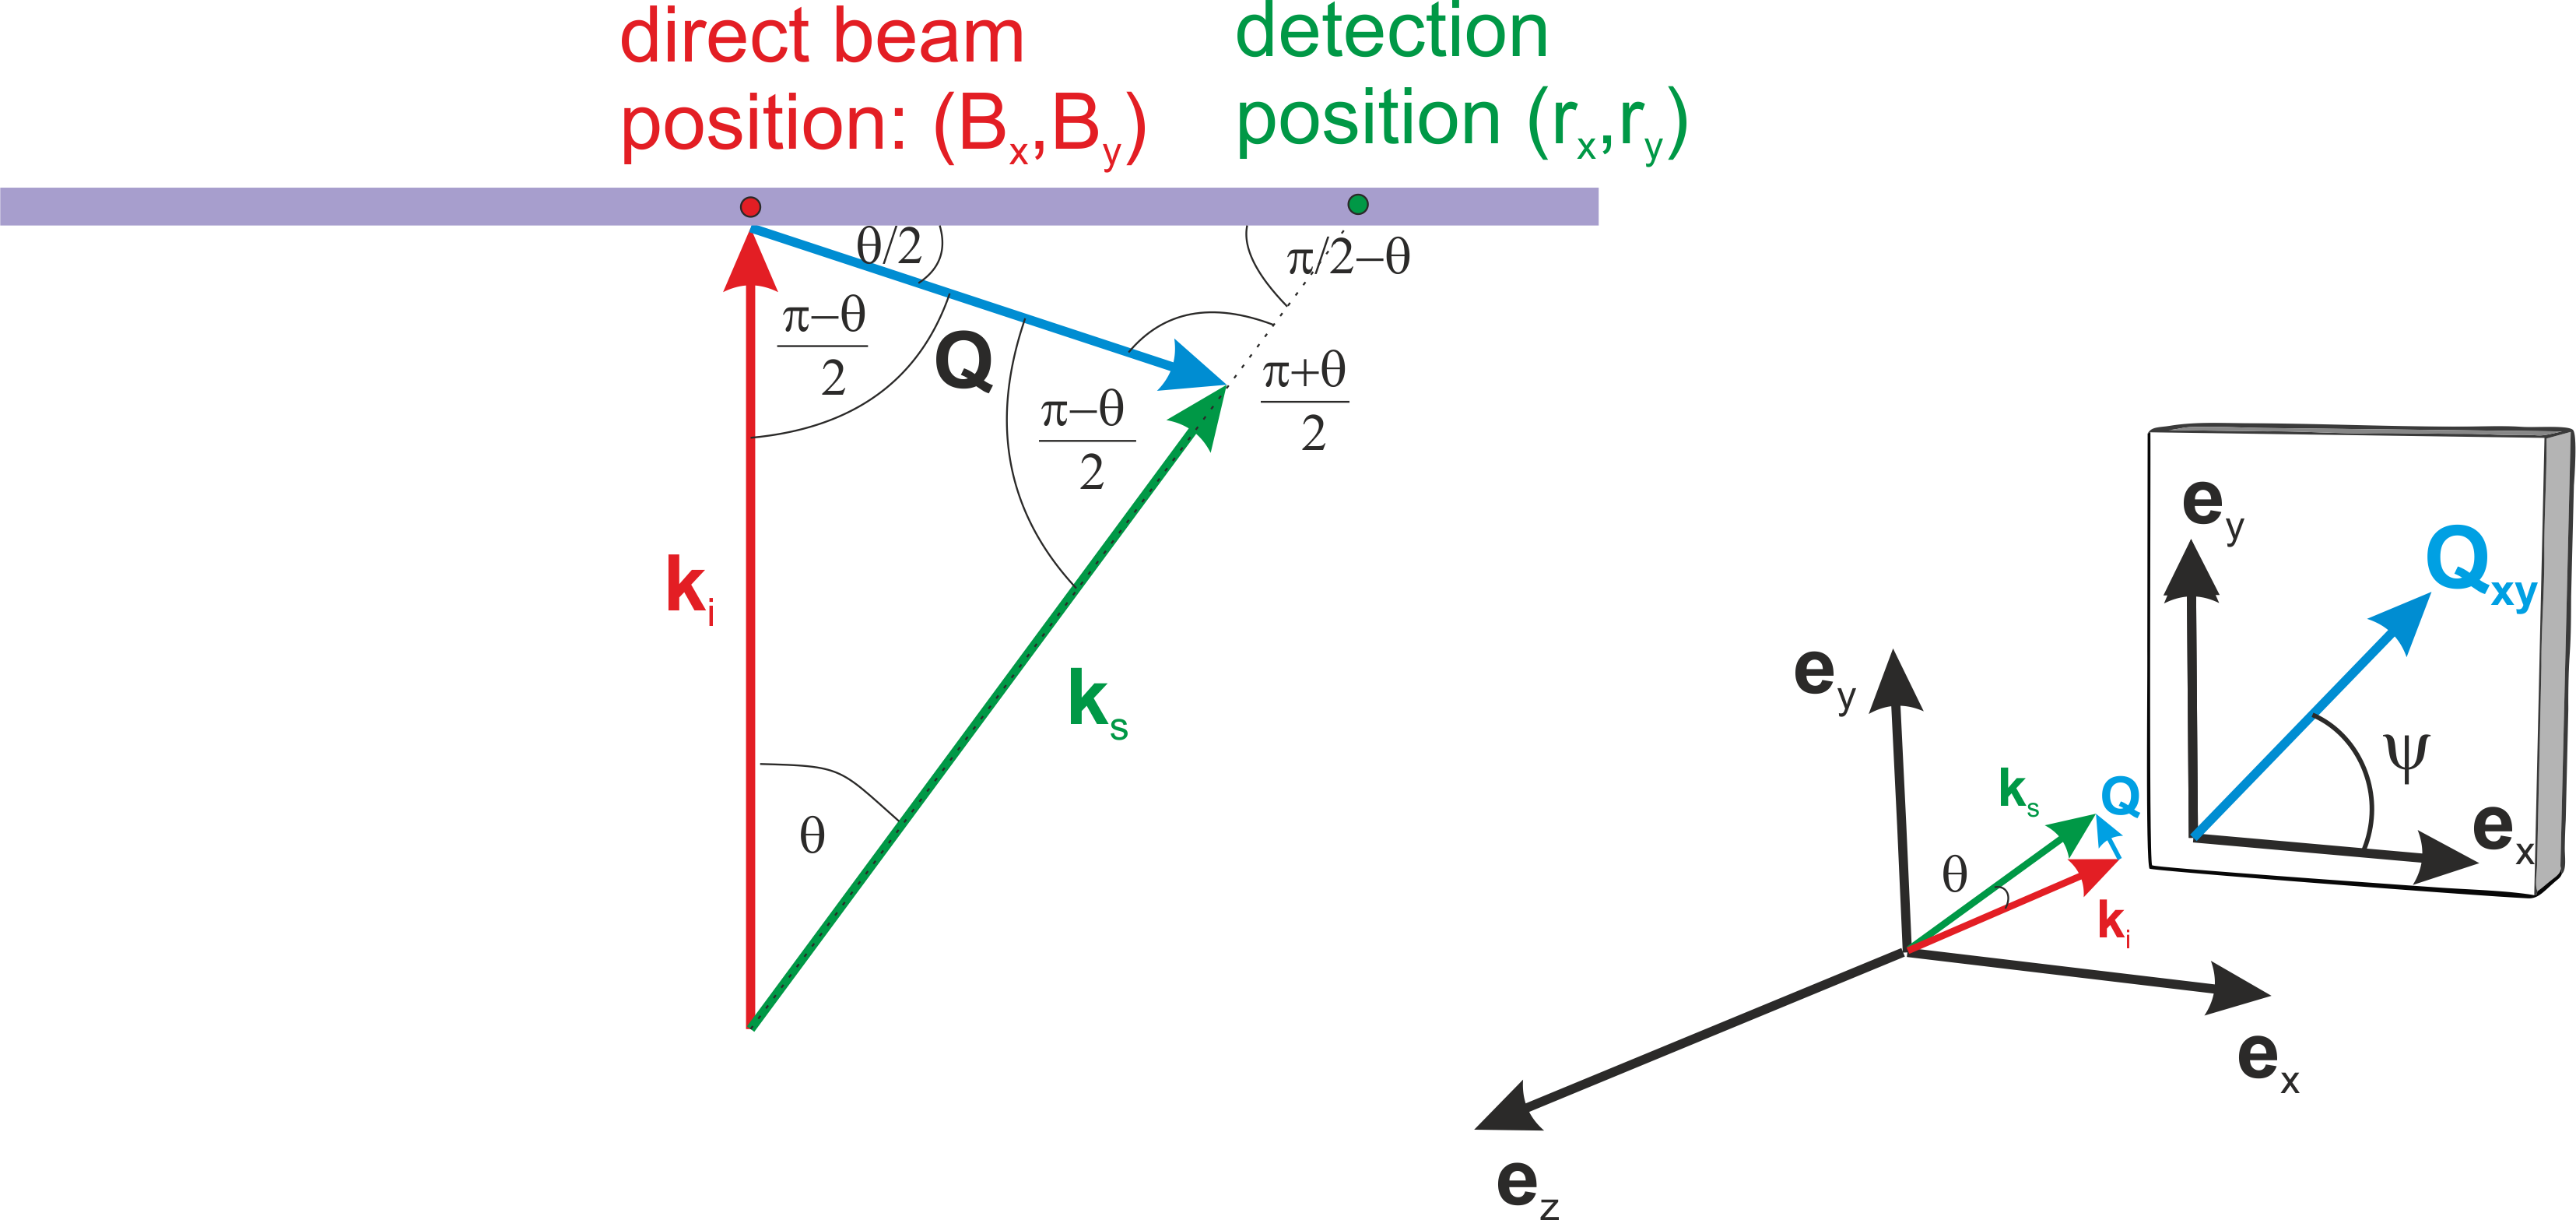
\includegraphics[width=0.85\textwidth]{osp_coord_system.png}
\end{center}
\caption{The scattering vector in polar coordinates coordination system with respect to a laboratory-fixed coordinate system based on the three orthogonal unit vectors ($\mathbf{e}_x$, $\mathbf{e}_y$, $\mathbf{e}_z$). They are arranged such that the x-direction coincides with the x-direction of the detector, and the y-direction coincides with the y-direction of the detector. The direction of the incoming neutron beam is chosen to be $-\mathbf{e}_z$. } \label{fig:opsCoordSys}
\end{figure}

\begin{align}
\mathbf{k}_i &=
    \left(
        \begin{array}{c}
                  k_{i,x} \\
                  k_{i,y} \\
                  k_{i,z}
        \end{array}
    \right)
    = \frac{2\pi}{\lambda}
    \left(
        \begin{array}{c}
                  0\\
                  0 \\
                  -1
        \end{array}
    \right) \\
\mathbf{k}_s &=
    \left(
        \begin{array}{c}
                  k_{i,x} \\
                  k_{i,y} \\
                  k_{i,z}
        \end{array}
    \right)
    = \frac{2\pi}{\lambda}
    \left(
        \begin{array}{c}
                  \cos(\psi) \sin(\theta)\\
                  \sin(\psi) \sin(\theta) \\
                  -\cos(\theta)
        \end{array}
    \right) \\
\mathbf{Q} &= \mathbf{k}_s - \mathbf{k}_i =
    \left(
        \begin{array}{c}
                  Q_{x} \\
                  Q_{y} \\
                  Q_{z}
        \end{array}
    \right)
    = \frac{2\pi}{\lambda}
    \left(
        \begin{array}{c}
                  \cos(\psi) \sin(\theta)\\
                  \sin(\psi) \sin(\theta) \\
                  1-\cos(\theta)
        \end{array}
    \right)
\end{align} 